\documentclass{beamer}
\usepackage[spanish, mexico]{babel}
\usepackage{colortbl}
%Tablas
\usepackage[flushleft]{threeparttable}
\usepackage{makecell,booktabs}
\usepackage{booktabs}
\usepackage{array}
%%% Colores
\usepackage{xcolor}
\definecolor{AzulOscuro}{RGB}{45, 62, 80}
\definecolor{GrisClaro}{RGB}{240, 240, 240}
\definecolor{AzulGris}{RGB}{119, 136, 153}
\definecolor{TextoGris}{RGB}{60, 60, 60}
\definecolor{olive}{rgb}{0.3, 0.4, .1}
\definecolor{fore}{RGB}{249,242,215}
\definecolor{back}{RGB}{51,51,51}
\definecolor{title}{RGB}{255,0,90}
\definecolor{dgreen}{rgb}{0.,0.6,0.}
\definecolor{gold}{rgb}{1.,0.84,0.}
\definecolor{JungleGreen}{cmyk}{0.99,0,0.52,0}
\definecolor{BG}{cmyk}{0.85,0,0.33,0}
\definecolor{RawSienna}{cmyk}{0,0.72,1,0.45}
\definecolor{Magenta}{cmyk}{0,1,0,0}
\definecolor{UBC}{rgb}{0.04706, 0.13725, 0.26667} % UBC Blue (primary)
\definecolor{UBCgrey}{rgb}{0.3686, 0.5255, 0.6235} % UBC Grey (secondary)
\usepackage{amsfonts,amsmath,oldgerm}
\usepackage{mathrsfs}
\usepackage{tikz}
\usetikzlibrary{arrows.meta, positioning, shapes.misc}
 % Biblioteca para mejores puntas de flecha
 % Con este paquete las ecuaciones pueden centrarse independientemente del simbolo '=' en el entorno \begin{gather} \end{gather}
\usetheme{sintef}

\newcommand{\testcolor}[1]{\colorbox{#1}{\textcolor{#1}{test}}~\texttt{#1}}
\usefonttheme[onlymath]{serif}
\usepackage{ragged2e}
\titlebackground*{assets/back.png}

\newcommand{\hrefcol}[2]{\textcolor{cyan}{\href{#1}{#2}}}
\vspace{-1cm}
\title{\small \centering \fontfamily{ptm}\selectfont Estudio \textit{in silico} del C\textsubscript{60} funcionalizado con glicina: propiedades relacionadas con la estructura electrónica, acoplamiento con la proteína NS2B-NS3 del virus del \textit{Dengue} y dinámica molecular}
\subtitle{Seminario de tesis I \\ Maestría en Ciencia y Tecnología}
\course{\textbf{Director de Tesis:} \\ Dr. Zuriel Natanael Cisneros García\\ \textbf{Codirector de Tesis:} \\ Dr. Carlos Iván Mendez Barrientos}
\author{Estefanía Espinoza Carmona}
\IDnumber{213449821}
\date{\small Lagos de Moreno, Jal., Mex. a 29 de mayo del 2026}
\usepackage{gensymb}
\usepackage{multirow} 
\usepackage{geometry}


\usepackage{graphicx}
\usepackage{adjustbox}

\usepackage{booktabs}




\begin{document}
\maketitle

\section{Introducción}
\begin{frame}{Introducción}
\begin{columns}[t]
\begin{column}{0.3\textwidth}
\begin{figure}
    \centering
    \includegraphics[width=0.8\textwidth, height=0.8\textwidth]{~/Tesis-Template-2/imagenes/Intro/fullereno.png} 
  \textbf{  \caption{\justifying Representación geométrica del fullereno C\textsubscript{60}.}}
    \label{int:1} %Esto genera un numero a mi etiqueta
\end{figure}
\end{column}

\begin{column}{0.3\textwidth}
\vspace*{-1cm}
   \begin{figure}
    \centering
    \includegraphics[width=0.9\textwidth, height=0.5\textwidth]{~/Tesis-Template-2/imagenes/Intro/biomedica.png} 
    \textbf{\caption{\justifying Estructura y actividad del aducto C\textsubscript{60} con aminoácidos. }}
    \label{bb} %Esto genera un numero a mi etiqueta
\end{figure}

\vspace*{-0.5cm}


\center
Propiedades biomédicas
\begin{itemize}
        \footnotesize
        
        % He usado el color 'blue' que es estándar, pero puedes cambiarlo por 'cyan'
        \item[{\color{blue}\tiny\textbullet}] Inducir la apoptosis
        \item[{\color{blue}\tiny\textbullet}] Acción antiviral
        \item[{\color{blue}\tiny\textbullet}] Propiedades antibacterianas
        \item[{\color{blue}\tiny\textbullet}] Antioxidantes
    \end{itemize}
    
 
\end{column}

\begin{column}{0.3\textwidth}
\vspace*{-1cm}
\begin{figure}
    \centering
    \includegraphics[width=1.0\textwidth, height=1.0\textwidth]{~/Tesis-Template-2/imagenes/Intro/inhibidor-denv2.png} 
    \textbf{\caption{\justifying Estructura del conjugado del ácido glicirrícico con el éster dimetílico del ácido L-glutámico como agente antiviral del DENV2.}}
    
    \label{bb} %Esto genera un numero a mi etiqueta
\end{figure}
\vspace*{-0.1cm}
\scriptsize{\cite{contreras2021aspectos}Lin et al., \textit{Viruses}, 2024.}
\end{column}
% There could be more!
\end{columns}

\end{frame}


%----------------------------------------------------------



%-------------------------------------------------------------------------------------------------

\section{Antecedentes}
\begin{frame}{Virus del Dengue}
\begin{columns}[t]
\begin{column}{0.4\textwidth}
\begin{figure}
    \centering
    \includegraphics[width=1.0\textwidth, height=0.5\textwidth]{~/Tesis-Template-2/imagenes/Intro/dengue.png} 
  \textbf{  \caption{\justifying Representación del mosquito hembra \emph{Aedes aegypti}.}}
    \label{int:1} %Esto genera un numero a mi etiqueta
\end{figure}
\scriptsize{\cite{contreras2021aspectos} Contreras et al., \textit{QhaliKay. Revista de Ciencias de la Salud}, 2021.}
\\
\scriptsize{\cite{arora2020two} Arora et al., \textit{Journal of Virology}, 2020.}\\

\end{column}

\begin{column}{0.5\textwidth}
\justifying \vspace{-1cm} \\
El virus del dengue es un flavivirus que pertenece a la familia Flaviviridae, el cual se puede clasificar por el complejo antigénico de reconocimiento en cuatro serotipos \cite{contreras2021aspectos, arora2020two}. 

\begin{figure}
    \centering
    \includegraphics[width=0.9\textwidth, height=0.6\textwidth]{~/Tesis-Template-2/imagenes/Ante/diagrama-1.png} 
    \textbf{\caption{\justifying Diferenciación antigénica de los serotipos del DENV\cite{contreras2021aspectos}.}}
    \label{bb} %Esto genera un numero a mi etiqueta
\end{figure}
\end{column}
% There could be more!
\end{columns}

\end{frame}
%--------------------------------------------------------------------------------------


\begin{frame}{Panorama Epidemiológico en México}
\begin{columns}
\begin{column}{0.6\textwidth}
\begin{table} % <--- Este es el que faltaba abrir
    \centering
    \scriptsize 
    \renewcommand{\arraystretch}{1.3} 
    \setlength{\tabcolsep}{3pt} 
    
    \caption{Casos y Defunciones al corte de la Semana 14; México, 2025 - 2026.}
    \resizebox{\linewidth}{!}{
    \begin{tabular}{l  c  c  c  c  c}
        \rowcolor[HTML]{800000} 
        \color{white}\textbf{Indicador} & 
        \color{white}\textbf{\shortstack{Casos \\ nuevos}} & 
        \color{white}\textbf{\shortstack{Casos \\ acumulados \\ 2026}} & 
        \color{white}\textbf{Incidencia} &
        \color{white}\textbf{\shortstack{Casos \\ acumulados \\ 2025}} & 
        \color{white}\textbf{Incidencia} \\
        \hline
        
        \rowcolor[HTML]{F2F2F2} Probables & 704 & 14,440 & 10.74 & 26,246 & 19.68 \\
        \textbf{Confirmados} & & & & & \\
        \rowcolor[HTML]{F2F2F2} \hspace{0.2cm} Dengue no grave & 36 & 607 & 0.45 & 1,117 & 0.84 \\
        \hspace{0.2cm}  Dengue con signos de alarma / grave & 41 & 801 & 0.60 & 1,456 & 1.09 \\
        \rowcolor[HTML]{F2F2F2} \hspace{0.2cm} Total de casos & 78 & 1,408 & 1.05 & 2,573 & 1.93 \\
        Defunciones & 0 & 3 & 0.00 & 12 & 0.82 \\
        \rowcolor[HTML]{F2F2F2} Estimados & 141 & 2,779 & 2.07 & 6,722 & 5.04 \\
        \hline
    \end{tabular}
    }
\end{table} 
\vspace{1cm}
\scriptsize{\cite{DGE2026} Secretaría de Salud, DGE (2026). Informe sobre la situación del dengue.}
\end{column}
\begin{column}{0.4\textwidth}
\vspace*{-1cm}
\begin{figure}
    \centering
    \includegraphics[width=1\textwidth, height=1.02\textwidth]{~/Tesis-Template-2/imagenes/Ante/casos_confirmados.png} 
   \textbf{ \caption{\justifying Serotipos identificados e incidencia de casos confirmados por entidad federativa; México, 2026 \cite{DGE2026}.}}
    \label{sun} %Esto genera un numero a mi etiqueta
\end{figure}
\end{column}
\end{columns}
\end{frame}






\begin{frame}{Estructura del genoma del virus del dengue}

\begin{columns}
\justifying
\begin{column}{0.6\textwidth}

\vspace*{-0.5cm}
\begin{figure}
    \centering
    \includegraphics[width=1.1\textwidth, height=0.6\textwidth]{~/Tesis-Template-2/imagenes/Ante/proteinas-conformación.pdf} 
  \caption{\justifying\textbf{ El genoma del virus del dengue  \cite{dhole2024host}.}}
    \label{dete} %Esto genera un numero a mi etiqueta

\end{figure} 


\end{column}
\begin{column}{0.4\textwidth}
\justifying
El DENV es un virus envuelto, con tamaño de virión de 50 nm, y contiene un ARN monocatenario de sentido positivo, de aproximadamente 11 kb de tamaño\cite{pourzangiabadi2025dengue}.\\
\vspace{2.5cm}


%\scriptsize{\cite{pourzangiabadi2025dengue} Pourzangiabadi et al., infection, Genetics and Evolution,2025.}
%\scriptsize{\cite{dhole2024host} Dhole et al., Inmmuno,2024}
\scriptsize{\cite{pourzangiabadi2025dengue} Pourzangiabadi et al., \textit{Infection, Genetics and Evolution}, 2025.}\\
\scriptsize{\cite{dhole2024host} Dhole et al., \textit{Immuno}, 2024.}


\end{column}
\end{columns}

\end{frame}


\begin{frame}{ Actividad de la proteína NS2B-NS3}
\begin{figure}[h]

    \centering
    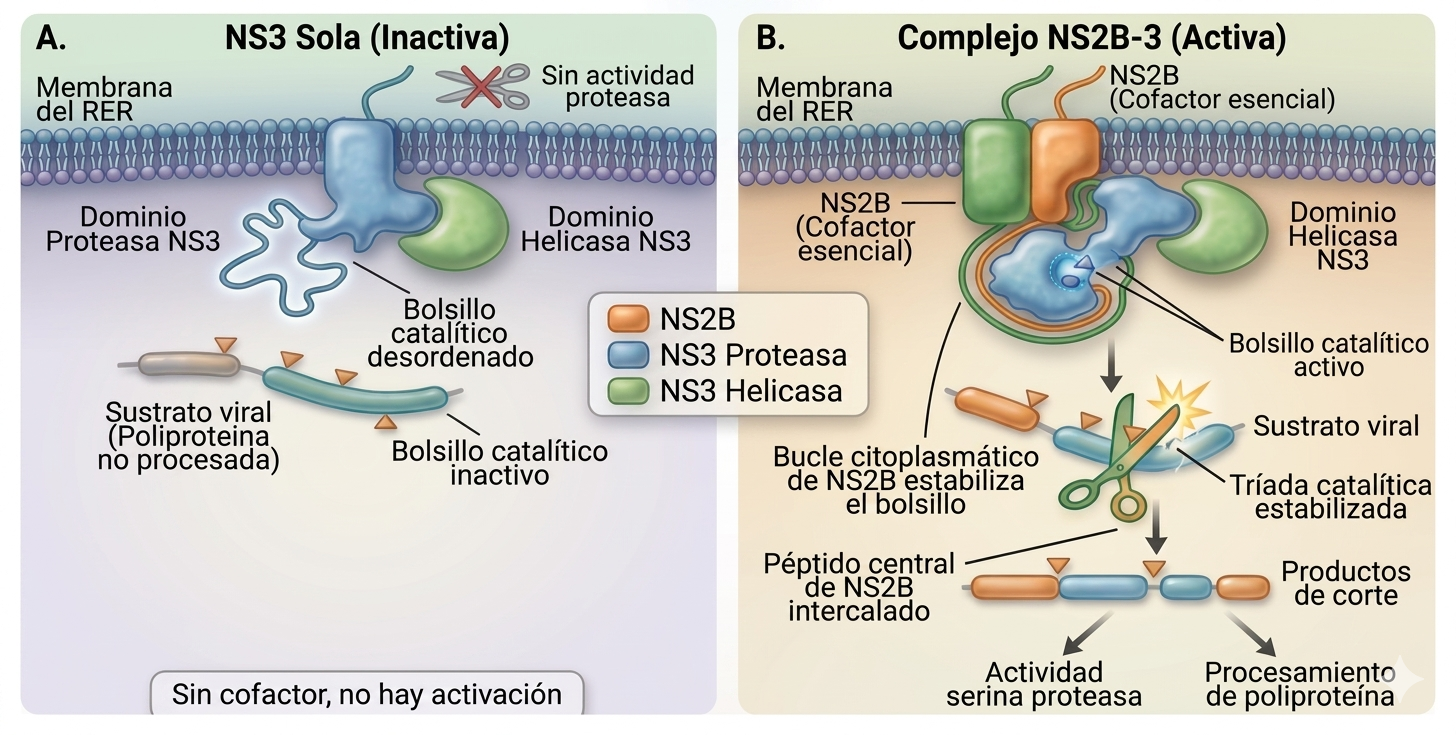
\includegraphics[width=0.8\textwidth,height=0.4\textwidth]{imagenes/Intro/ns2b-ns3-1.png}
\caption{\justifying \textbf{Activación crítica de la Serina Proteasa NS3 por el cofactor NS2B.}}
\end{figure}
\end{frame}
%Figura 1 | Ciclo de vida del virus del dengue. El virus del dengue existe en diversas formas virales, dependiendo del grado de escisión de la proteína precursora de membrana (prM). Las partículas virales inmaduras del dengue contienen un conjunto completo de proteínas prM y no son infecciosas, mientras que en las partículas virales maduras, todas las proteínas prM están escindidas.
%Existen varias formas intermedias, parcialmente maduras, en las que algunas proteínas prM se han escindido y otras permanecen intactas. Las partículas virales maduras y algunas parcialmente maduras son infecciosas (paso 1). El proceso de replicación del virus del dengue comienza cuando un virión se une directamente a diversos receptores de la célula huésped o cuando la porción Fc de un complejo inmune que contiene el virus del dengue se une a un receptor Fc en las células diana (paso 2) y posteriormente ingresa a la célula mediante endocitosis mediada por receptores (paso 3). La acidificación de las vesículas endosomales desencadena
%cambios conformacionales en el virión, lo que resulta en una
%trimerización irreversible de la proteína de la envoltura viral (E) (no se muestra). Esto expone
%el péptido de fusión y media la fusión entre las membranas viral y endosomal, permitiendo la liberación de la nucleocápside en
%el citoplasma. El ARN viral se libera en el citoplasma y se presenta
%al retículo endoplasmático rugoso (RE) (paso 4). En el RE, el ARN viral se
%traduce en una única poliproteína que es procesada por proteasas virales y del huésped (paso 5). Una vez sintetizado el complejo de replicación viral, la traducción del ARN viral se
%desactiva y comienza la síntesis de ARN mediante la
%transcripción de un ARN viral antisentido, seguida de la amplificación del ARN viral (paso 6). El ARN recién sintetizado es posteriormente empaquetado
%por la proteína de la cápside (C), formando una nucleocápside (paso 7). El ensamblaje del virus ocurre en la superficie del RE cuando la nucleocápside brota hacia el lumen del RE,
%dando como resultado partículas virales inmaduras no infecciosas (paso 8).
%Las partículas virales inmaduras se transportan a través del aparato de Golgi hacia la
%red trans-Golgi, donde la acidificación induce cambios conformacionales
%del virión y expone los sitios de escisión de la furina. La proteasa del huésped, la furina,
%escinde entre la proteína pr y la proteína M, permaneciendo la proteína pr
%asociada hasta que el virión se libera en el pH neutro del medio extracelular (paso %9). DC-SIGN, proteína no integrina específica de células dendríticas que se une a ICAM3; proteínas NS, proteínas no estructurales.

\begin{frame}{ Actividad de la proteína NS2B-NS3}
\begin{figure}[h]

    \centering
    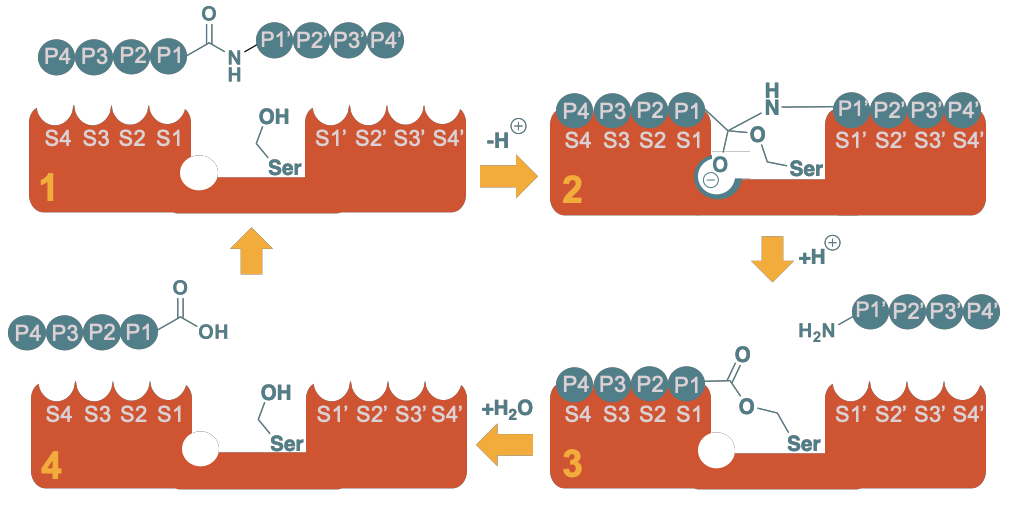
\includegraphics[width=0.8\textwidth,height=0.4\textwidth]{imagenes/Intro/serina.png}
\caption{\justifying \textbf{Representación de la proteolisis de un péptido por una serina proteasa.}}
\end{figure}
\end{frame}
%------------------------------------------------------------------------------
\begin{frame}{Estructura de la proteína NS2B-NS3}
\justifying
%Los 170 aa del extremo N-terminal de NS3 presentan actividad proteasa, y un núcleo hidrofóbico de aproximadamente 40 aa dentro de NS2B proporciona una función de cofactor esencial\cite{brecher2013flavivirus}.\\

\begin{columns}
\begin{column}{0.20\textwidth}
\vspace*{-1cm}
\begin{itemize}
    \item \textbf{Serina proteasa}
    \item \textbf{Geometría} 
    \item \textbf{Estabilizar} 
    \item \textbf{Activa} 
\end{itemize}
\end{column}


\justifying
\begin{column}{0.40\textwidth}
\begin{figure}
    \centering
    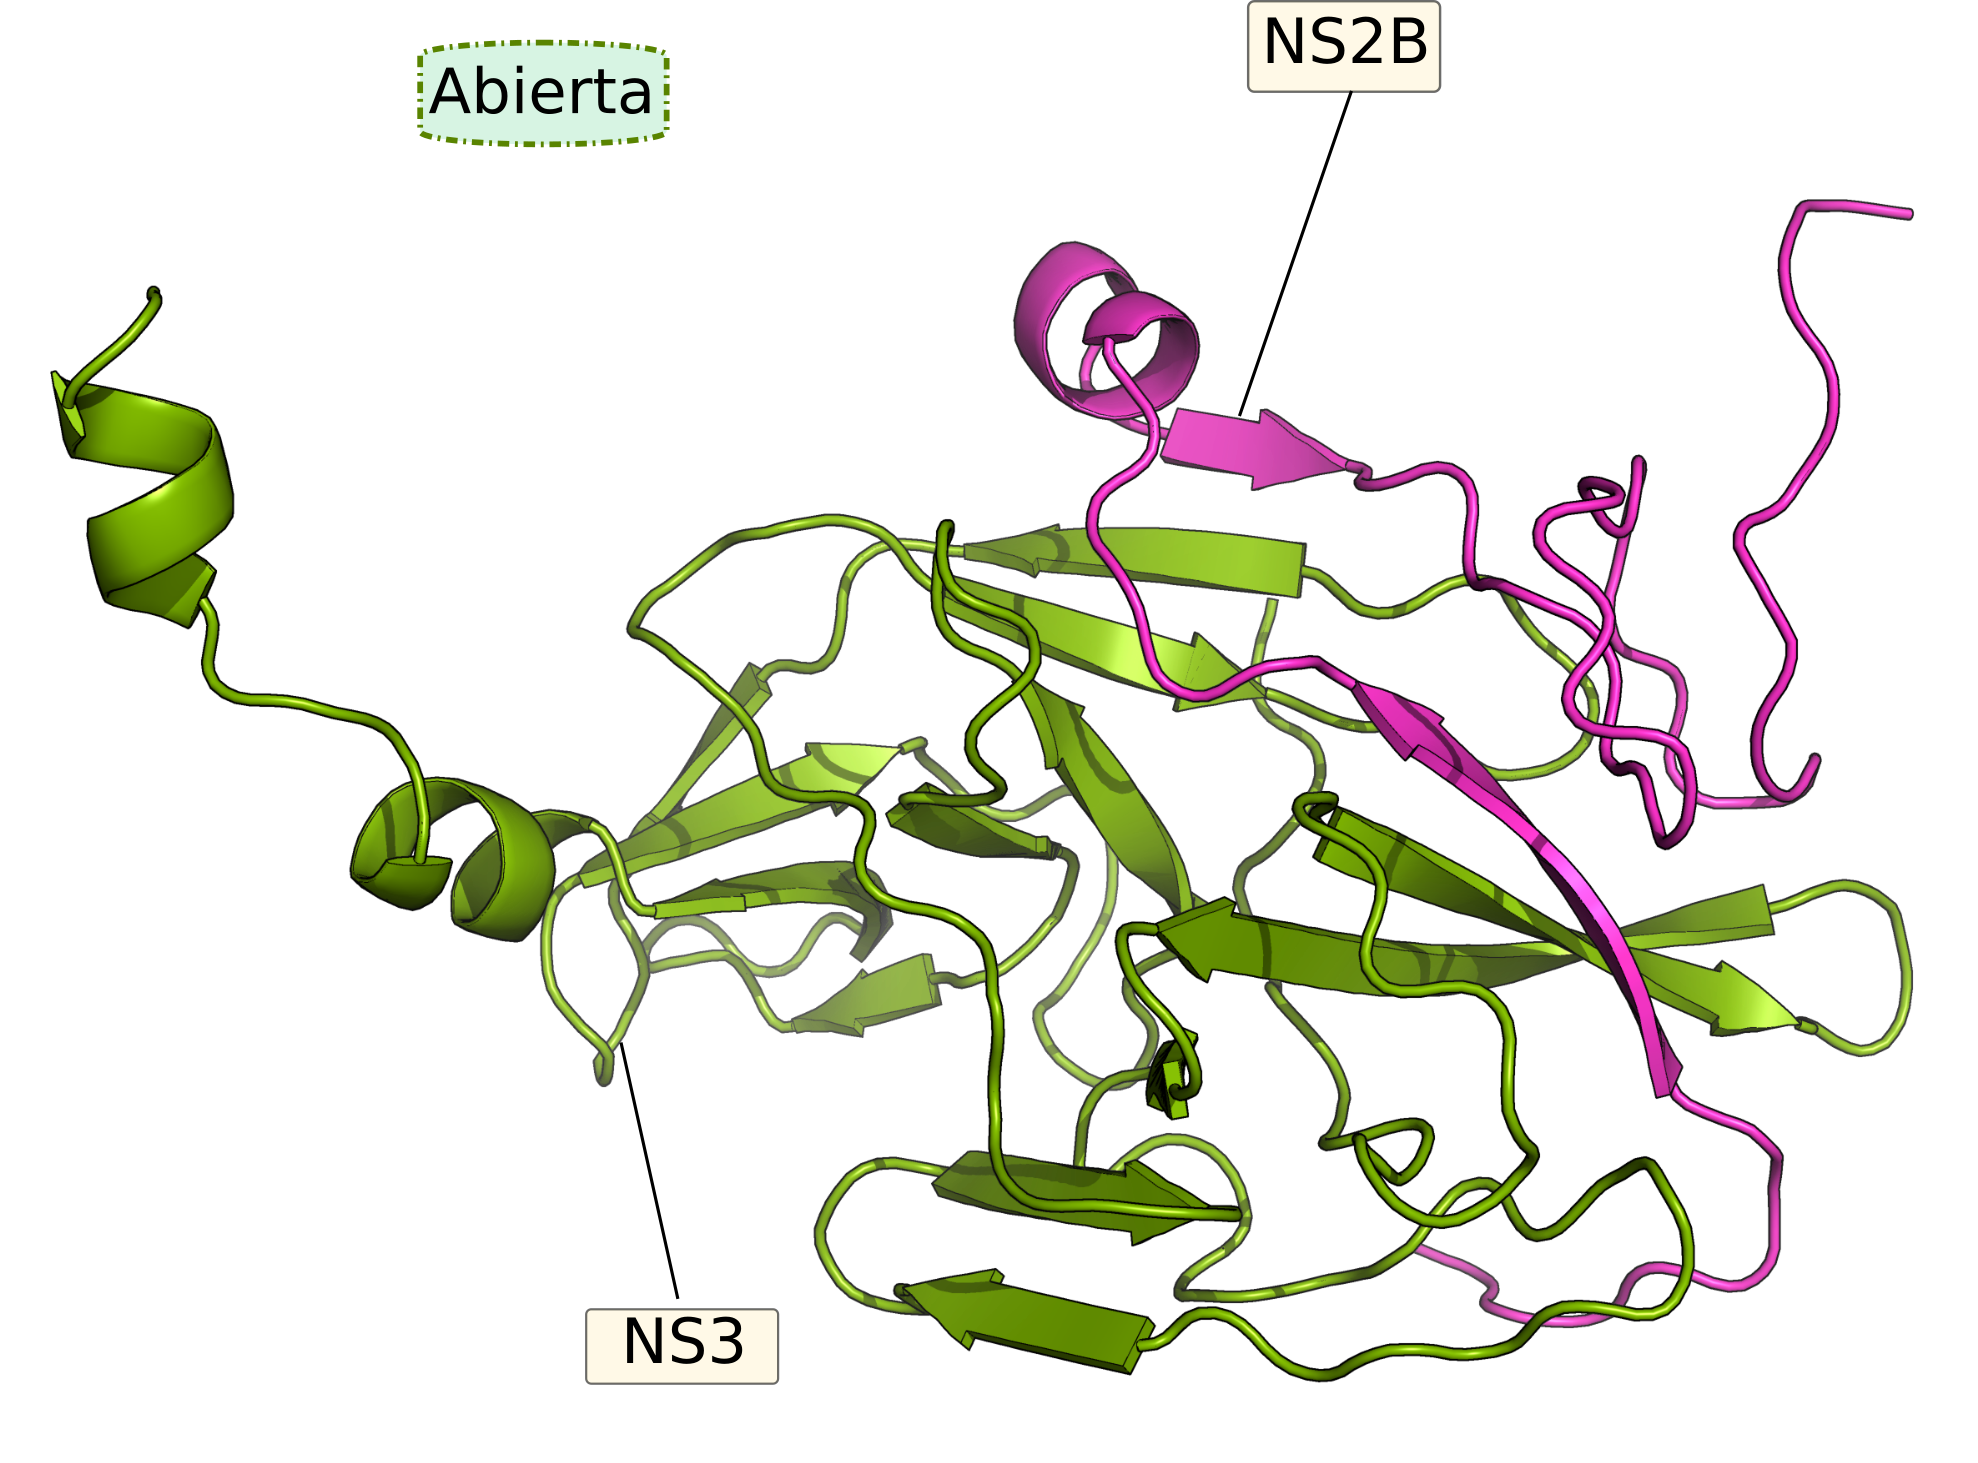
\includegraphics[width=1.0\textwidth, height=1.0\textwidth]{imagenes/Intro/proteina-2FOM.png} 
   \textbf{ \caption{\justifying Estructura de la proteína 2FOM.}}
    \label{dete} %Esto genera un numero a mi etiqueta
\end{figure} 
\end{column}


\justifying
\begin{column}{0.40\textwidth}
\vspace*{-1cm}
\begin{figure}
    \centering
    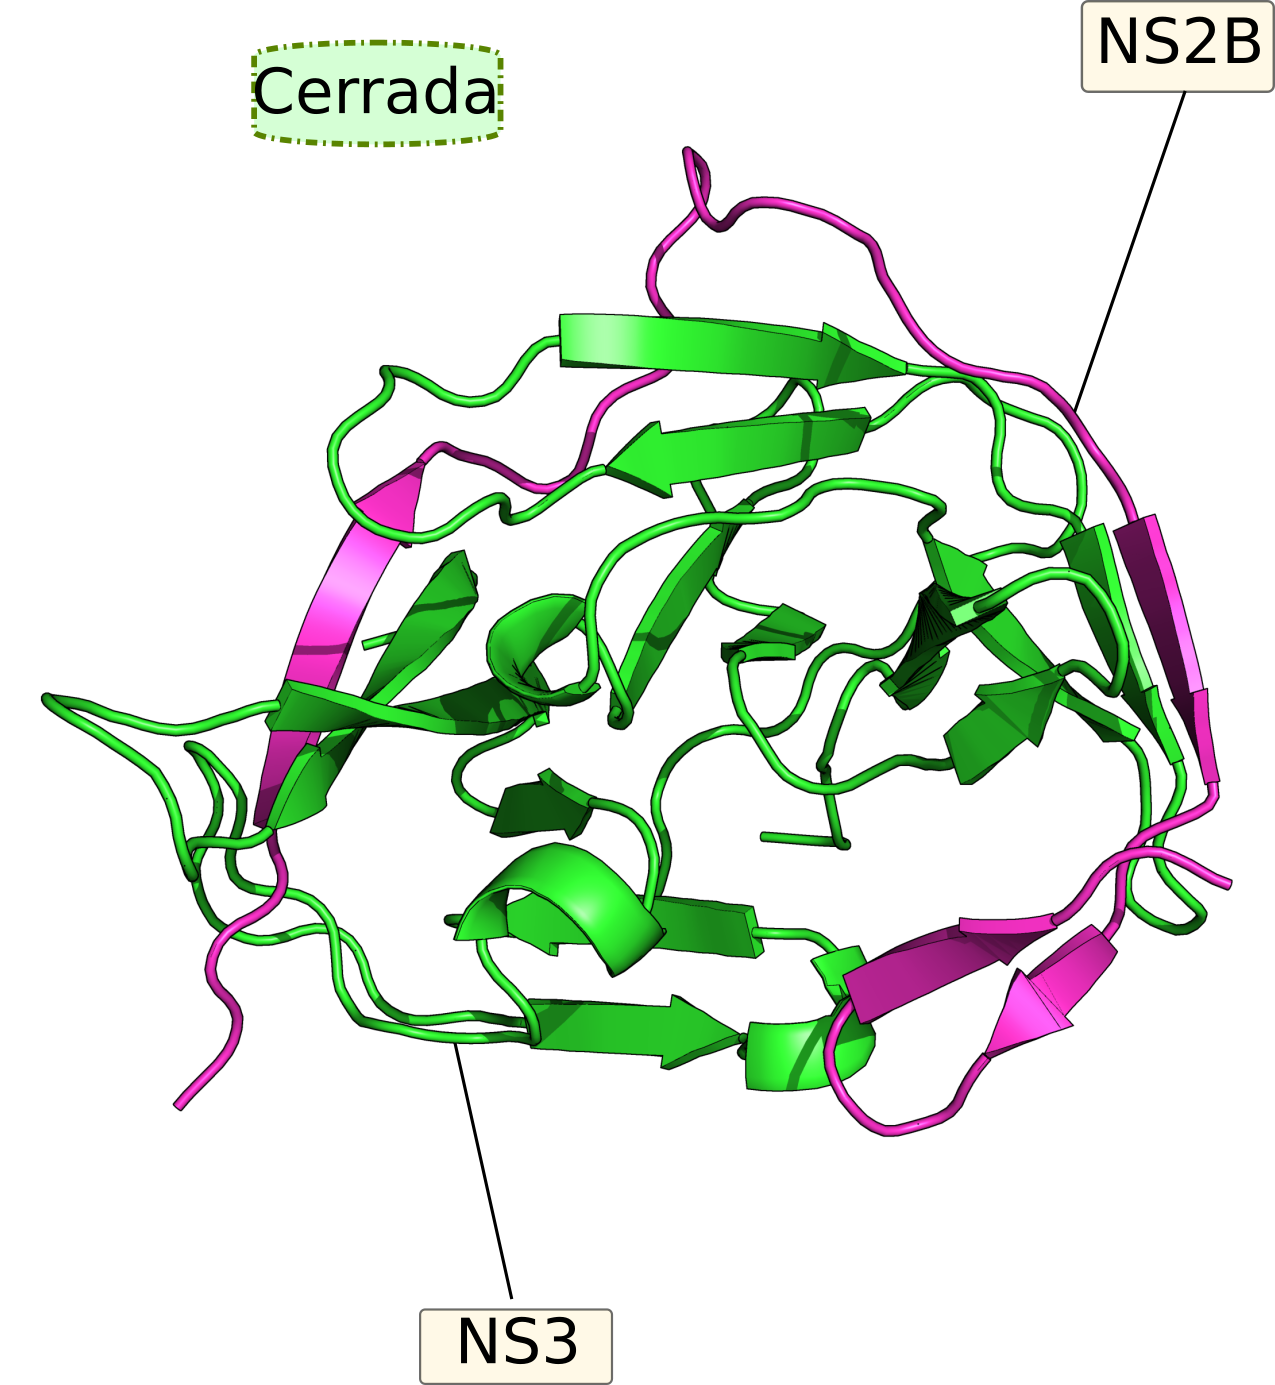
\includegraphics[width=1.0\textwidth, height=1.0\textwidth]{imagenes/Intro/proteina-2FP7.png} 
  \textbf{  \caption{\justifying Estructura de la proteína 2FP7.}}
    \label{dete} %Esto genera un numero a mi etiqueta
\end{figure} 
\end{column}
\justifying
\end{columns}
\end{frame}
%%---------------------------------------------------------
\begin{frame}{Residuos clave en la inhibición de DENV2}
\begin{columns}
\begin{column}{0.6\textwidth}
\begin{figure}[h]
    \centering
    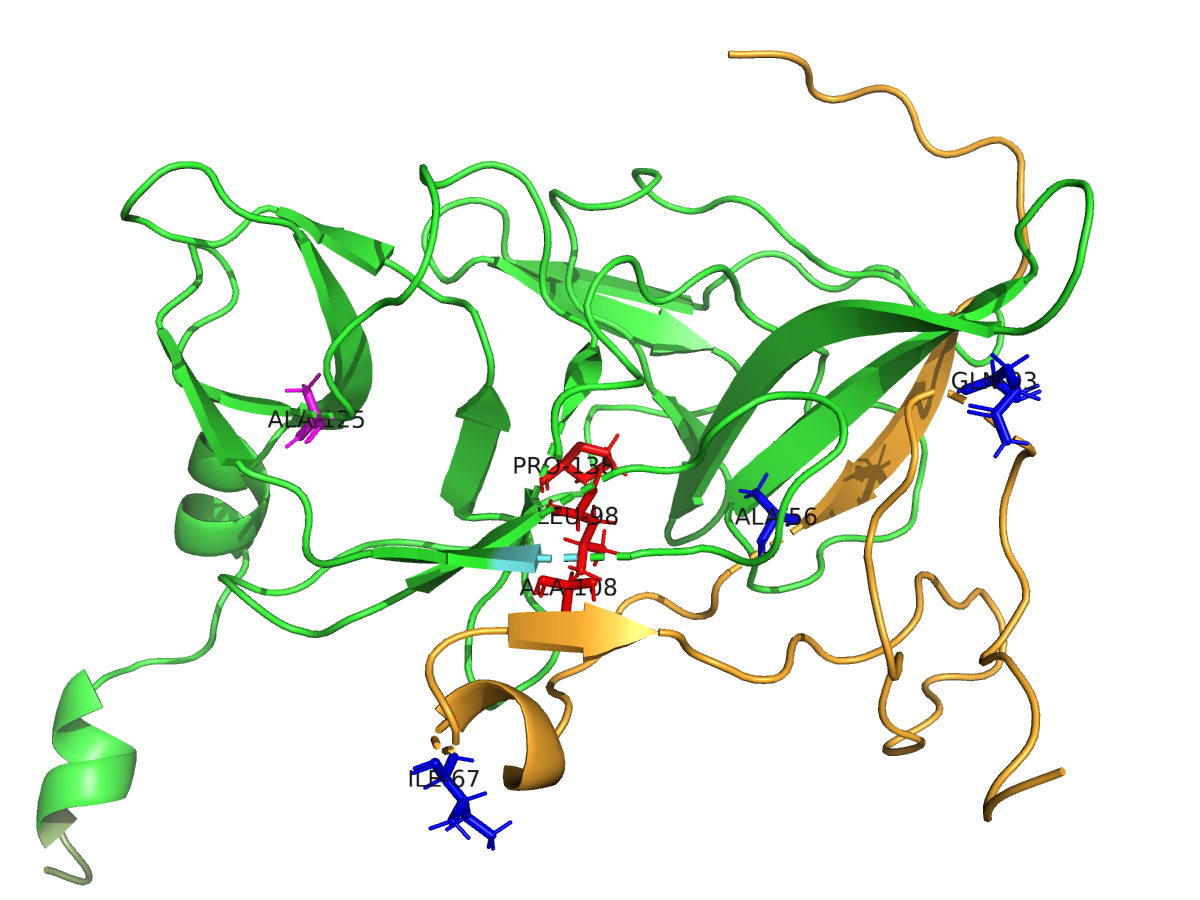
\includegraphics[width=0.8\textwidth,height=0.6\textwidth]{imagenes/Intro/proteina-sitio-alosterico-1.pdb.png}
     \textbf{\caption{Residuos identificados en la inhibición alostérica de la proteína NS2B-NS3 en conformación abierta. }}
\end{figure}
 
\end{column}
\begin{column}{0.4\textwidth}

\justifying
 Se identificaron como residuos críticos para la formación del complejo. 


\vspace{0.25cm}
\centering
\textcolor{gold}{NS2B}
\begin{itemize}
\footnotesize
\item \textcolor{black}{Ala56\begin{tikzpicture} \draw[-{Stealth[scale=1.0]}, thick, blue] (0,0) -- (1,0); \end{tikzpicture} no polar alifático}
\item \textcolor{black}{Ile67 \begin{tikzpicture} \draw[-{Stealth[scale=1.0]}, thick, blue] (0,0) -- (1,0); \end{tikzpicture} no polar alifático}
\item \textcolor{black}{Gln93\begin{tikzpicture} \draw[-{Stealth[scale=1.0]}, thick, blue] (0,0) -- (1,0); \end{tikzpicture} polar no cargado} 
\end{itemize} 
\centering
\textcolor{green}{NS3}
\begin{itemize}
\footnotesize
\item \textcolor{black}{Leu98\begin{tikzpicture} \draw[-{Stealth[scale=1.0]}, thick, blue] (0,0) -- (1,0); \end{tikzpicture} no polar alifático}
\item \textcolor{black}{Ala108 \begin{tikzpicture} \draw[-{Stealth[scale=1.0]}, thick, blue] (0,0) -- (1,0); \end{tikzpicture} no polar alifático}
\item \textcolor{black}{Pro138\begin{tikzpicture} \draw[-{Stealth[scale=1.0]}, thick, blue] (0,0) -- (1,0); \end{tikzpicture} no polar alifático} 
\end{itemize} 
\vspace*{1cm}
\scriptsize{\cite{jonniya2022functional}Jonniya, N. \& Kar, P.,\emph{Journal of Chemical Information and Modeling, 2022.}}
\end{column}
\end{columns}
\end{frame}
%-------------------------------------------------


%--------------------------------------------------------------------------------------------------------------------
\begin{frame}{Residuos clave en la inhibición de DENV2}
\vspace*{-2cm}
\begin{columns}
\begin{column}{0.7\textwidth}
\vspace*{1cm}
\begin{figure}[h]
    \centering
    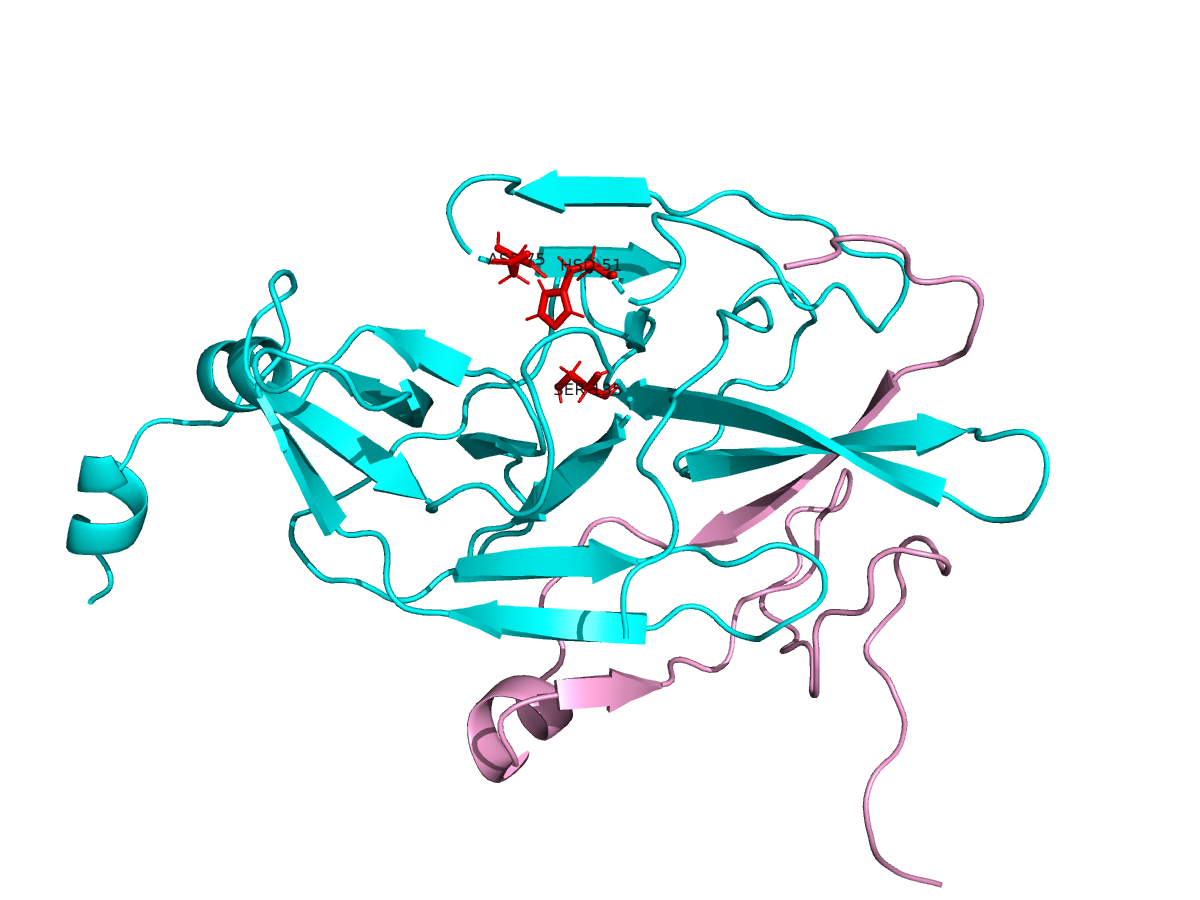
\includegraphics[width=0.9\textwidth,height=0.7\textwidth]{imagenes/Intro/proteina-ortoesterico.png}
     \textbf{\caption{Residuos identificados en la inhibición ortostérica de la proteína NS2B-NS3 en conformación abierta. }}
\end{figure}
\end{column}
\begin{column}{0.4\textwidth}

\justifying
\vspace*{1.5cm}
Las regiones del sitio activo corresponden a los aminoácidos en color rojo de la Figura 13. 
\vspace{1.5cm}
\begin{itemize}
\footnotesize
\item \textcolor{black}{His51\begin{tikzpicture} \draw[-{Stealth[scale=1.0]}, thick, blue] (0,0) -- (1,0); \end{tikzpicture} polar básico positivo}
\item \textcolor{black}{Asp75 \begin{tikzpicture} \draw[-{Stealth[scale=1.0]}, thick, blue] (0,0) -- (1,0); \end{tikzpicture} ácido negativo}
\item \textcolor{black}{Ser135 \begin{tikzpicture} \draw[-{Stealth[scale=1.0]}, thick, blue] (0,0) -- (1,0); \end{tikzpicture} polar no cargado} 
\end{itemize} 
%\begin{tikzpicture}
    % Flecha básica
   % \draw[->] (0,1) -- (2,1);
    
    % Flecha con estilo personalizado (gruesa, color azul, punta stealth)
    %\draw[-{Stealth[scale=1.5]}, thick, blue] (0,0) -- (0.5,0);
    
    % Flecha doble curva
    %\draw[<->, >=latex, thick, red] (0,-0.5) to[out=30, in=150] (2,-0.5);
%\end{tikzpicture}
\vspace*{2cm}
\scriptsize{\cite{jonniya2022functional}Jonniya, N. \& Kar, P.,\emph{Journal of Chemical Information and Modeling}, 2022.}
\end{column}
\end{columns}

\end{frame}
%---------------------------------------------------------------------

\begin{frame}{Inhibidor ortostérico}
\begin{columns}
\begin{column}{0.4\textwidth}
\justifying
\textbf{Tipo de interacción:} Competitiva no covalente
\\
\textbf{Limitaciones:} mantener su selectividad \textit{in vivo} frente a las proteasas del huésped.
\end{column}
\begin{column}{0.6\textwidth}
\vspace*{-1cm}
\begin{figure}[h]
    \centering
    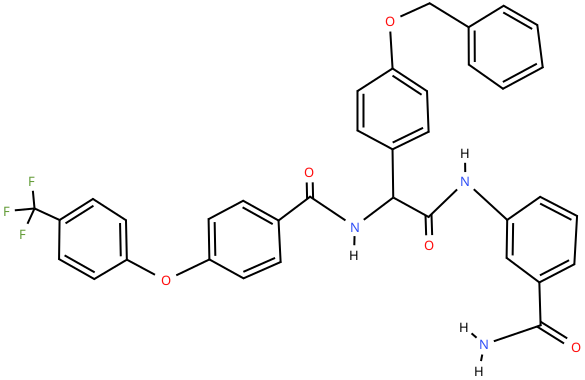
\includegraphics[width=0.8\textwidth,height=0.6\textwidth]{imagenes/Intro/inhibidor-b.png}
    \textbf{ \caption{Inhibidor ortostérico compuesto 71 (derivados pequeños de benzamida/fenilglicina).}}
    
  \scriptsize{\cite{zephyr2023allosteric} Zephyr, J. et al.,\emph{Bioorganic Chemistry}, 2023.}

\end{figure}
\end{column}
\end{columns}
\end{frame}
%-----------------------------------------------------
\begin{frame}{Inhibidor alostérico}
\begin{columns}
\begin{column}{0.5\textwidth}
\justifying
\textbf{Tipo de interacción}: No covalente. Interacciones hidrofóbicas que bloquean mecánicamente la transición de la enzima hacia su conformación activa cerrada. 
\end{column}
\begin{column}{0.5\textwidth}
\vspace*{-1cm}
\begin{figure}[h]
    \centering
    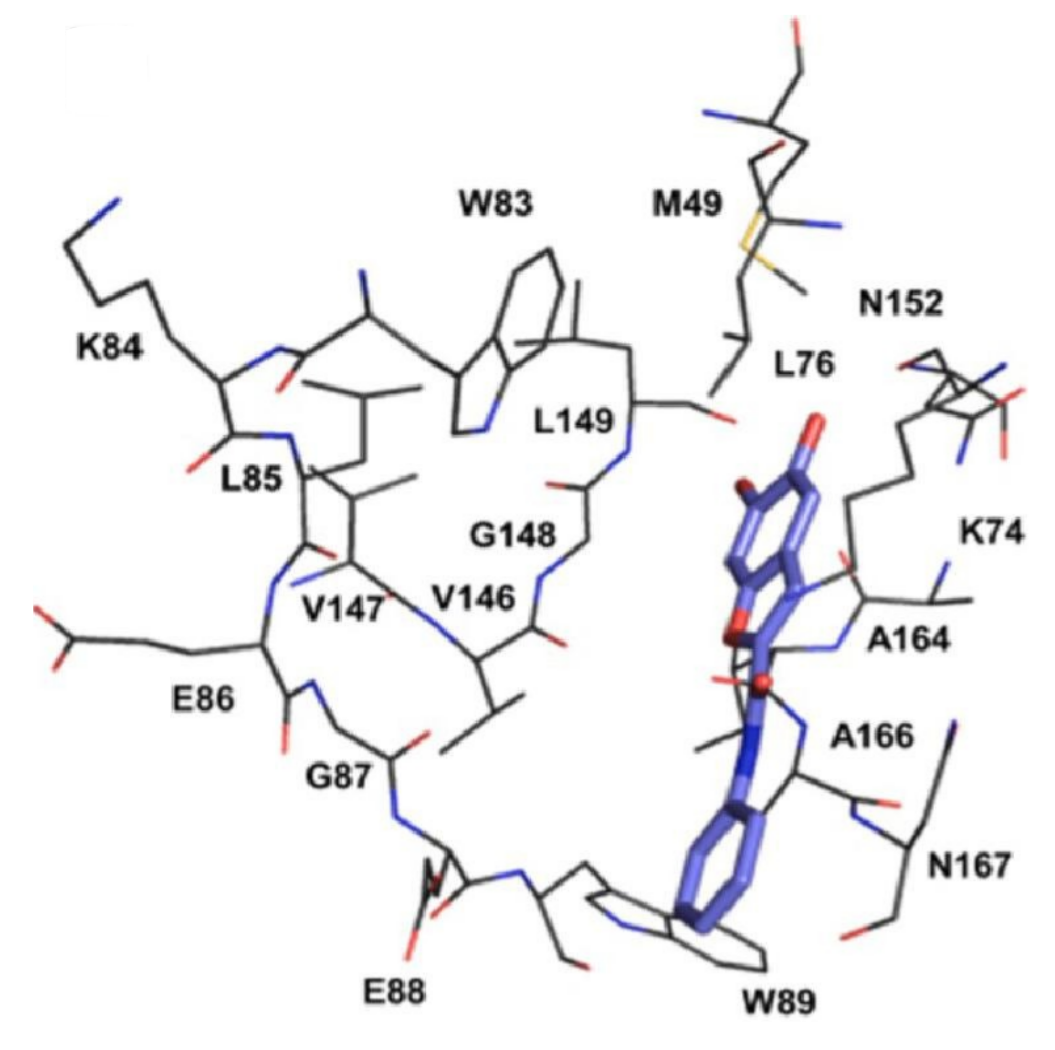
\includegraphics[width=0.5\textwidth,height=0.7\textwidth]{imagenes/Intro/inhibidor-3.png}
     \textbf{\caption{Inhibidor alostérico del compuesto 34e (derivado de benzofurano tipo amida).}}
     
 \scriptsize{\cite{maus2021sar} Maus, H. et al.,\emph{Bioorg. Med. Chem}, 2021.}
\end{figure}
\end{column}
\end{columns}
\end{frame}
%------------------------------------------------------------

%_------------------------------------------------------
\begin{frame}{Inhibidor alostérico}
\begin{columns}
\begin{column}{0.4\textwidth}
\justifying
\textbf{Tipo de interacción: }Interactúa mediante apilamiento $\pi$-$\pi$ con Tyr161 y hace contactos clave con Lys74 y Leu149, bloqueando el cierre de NS2B. 
\end{column}
\begin{column}{0.6\textwidth}
\vspace*{-1cm}
\begin{figure}[h]
    \centering
    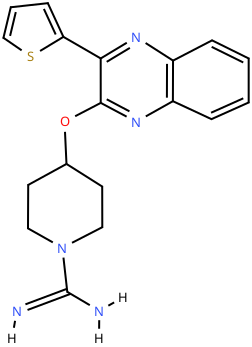
\includegraphics[width=0.5\textwidth,height=0.6\textwidth]{imagenes/Intro/inhibidor-c.png}
    \textbf{ \caption{Inhibidor alostérico: compuesto 32 (núcleo de quinoxalina-2(H)-ona).}}
  \scriptsize{\cite{cavina2024orthoflaviviral}Cavina, L. et al.,\emph{Molecules}, 2024.}

\end{figure}
\end{column}
\end{columns}
\end{frame}


%---------------------------------------------------------------
\begin{frame}{Inhibidor alostérico }
\begin{columns}
\begin{column}{0.6\textwidth}
\begin{figure}[h]
    \centering
    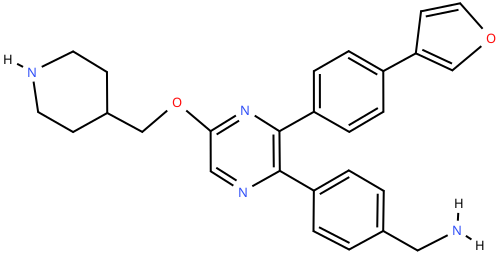
\includegraphics[width=0.7\textwidth,height=0.5\textwidth]{imagenes/Intro/inhibidor-a.png}
     \textbf{\caption{Inhibidor alostérico del compuesto JVJ derivado de pirazina.}}
\end{figure}
\end{column}
\begin{column}{0.5\textwidth}
\justifying
\textbf{Tipo de interacción:} Estabilización de conformación inactiva. Modifica la dinámica de los lazos, induciendo una forma \textquotedblleft abierta\textquotedblright\ e inactiva de la enzima.  
\begin{itemize}
    \item \textbf{PDB:} 6MO0
    \item \textbf{Cavidad alostérica:} Bucle 120s y 150s
\end{itemize}


\vspace*{2cm}
 \scriptsize{\cite{jonniya2022functional}Jonniya, N. \& Kar, P.,\emph{Journal of Chemical Information and Modeling}, 2022.}
\end{column}
\end{columns}
\end{frame}
%--------------------------------------------------------------------
\begin{frame}{Síntesis y caracterización del sistema C\textsubscript{60}(\textit{Gly})\textsubscript{4}}
\begin{columns}
\begin{column}{0.6\textwidth}

\begin{figure}[h]
    \centering
    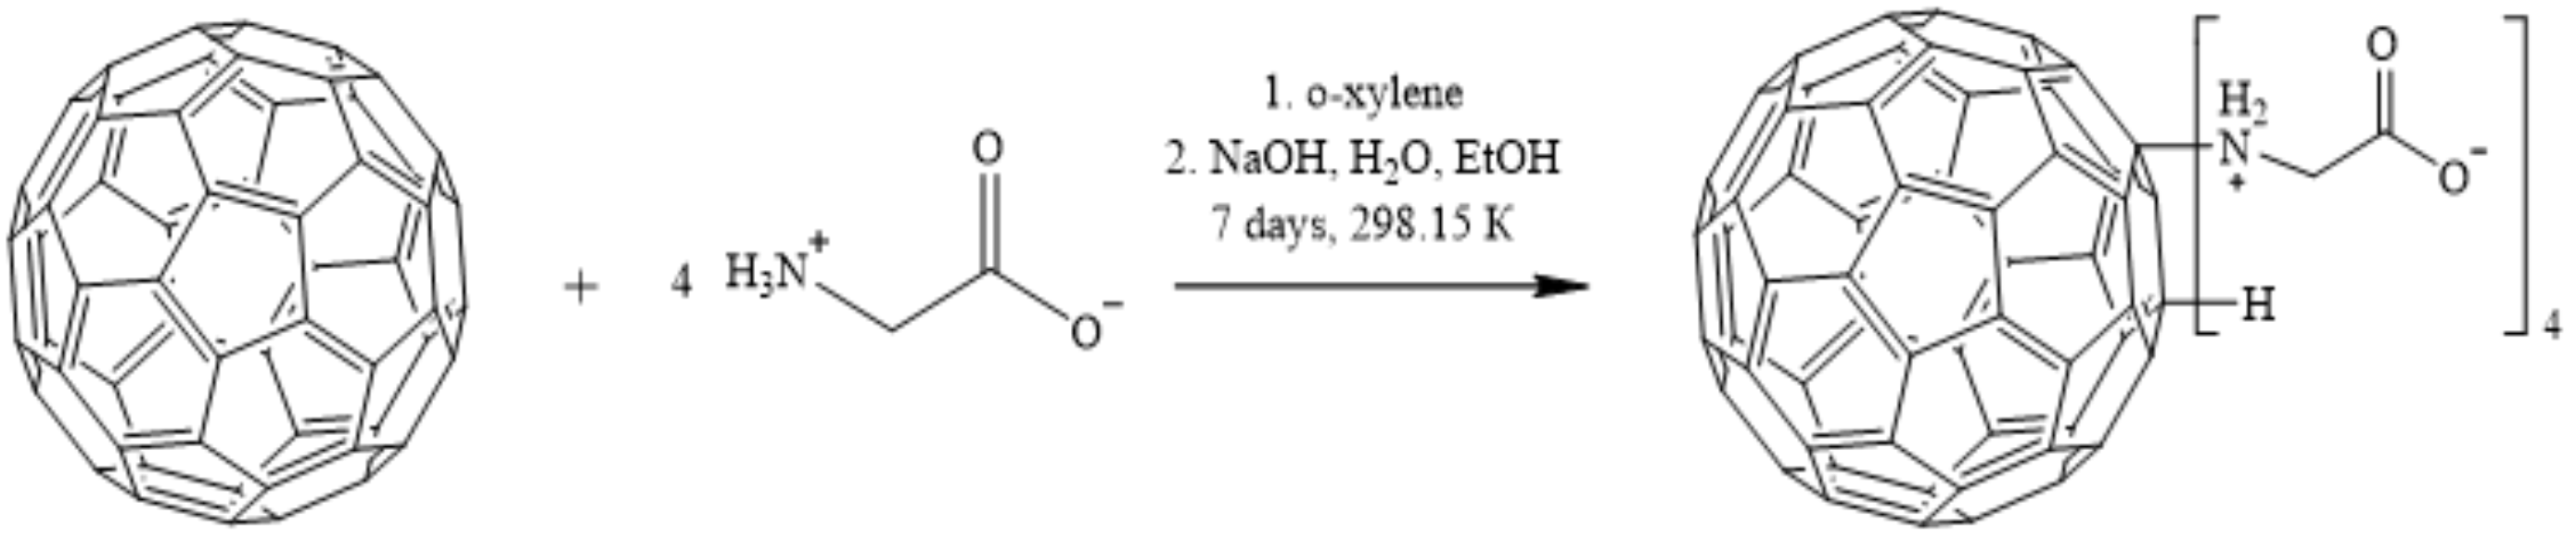
\includegraphics[width=0.9\textwidth,height=0.2\textwidth]{imagenes/Intro/sintesis.png}
    \textbf{\caption{Síntesis del C\textsubscript{60}(\textit{Gly})\textsubscript{4}.}
    \label{workin} }%Esto genera un numero a mi etiqueta
\end{figure}
\justifying
La solución resultante se purificó mediante membranas de diálisis durante tres días. 
El producto final se secó a 50~\textdegree C durante 24~h. El rendimiento del 
producto fue del 85\%.

\end{column}
\begin{column}{0.45\textwidth}
\vspace*{-0.5cm}
\begin{figure}[h]
    \centering
    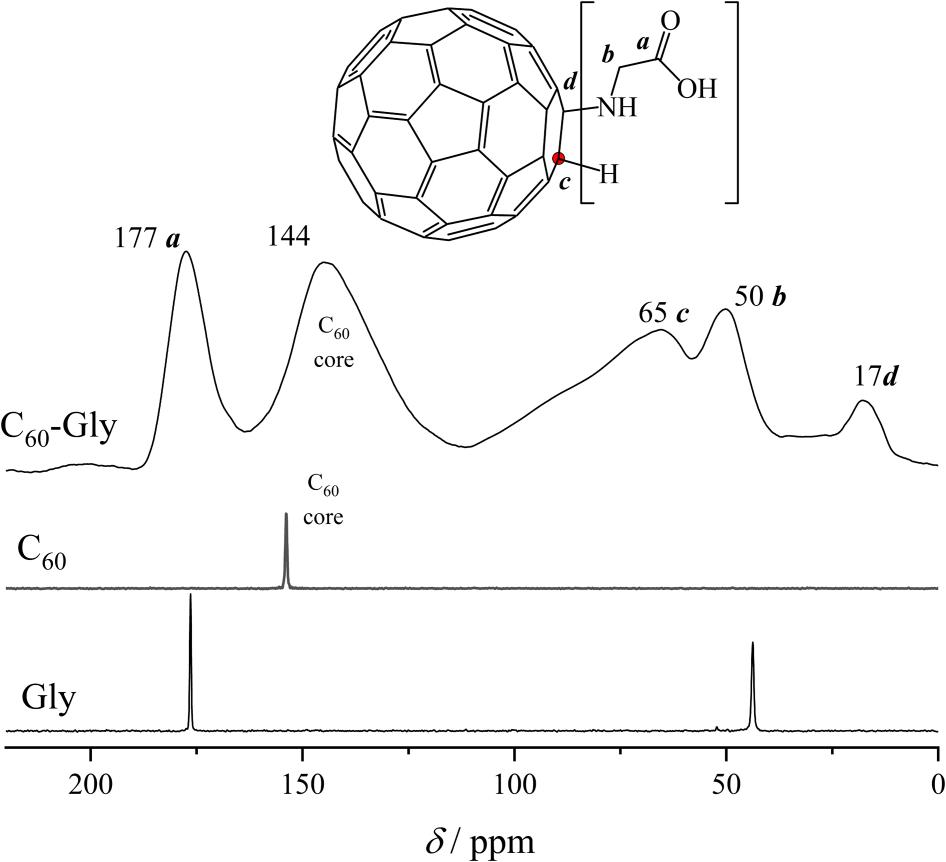
\includegraphics[width=0.8\textwidth,height=0.8\textwidth]{imagenes/Intro/NMR.png}
    \textbf{\caption{Espectro de RMN de \textsuperscript{13}C de C\textsubscript{60}, C\textsubscript{60}-Gly y Gly.}
    \label{workin} }%Esto genera un numero a mi etiqueta
\end{figure}
\scriptsize{\cite{sharoyko2024modification} Sharoyko, V. V. et al.} \textit{Fullerenes, Nanotubes and Carbon Nanostructures}, 2024.
\end{column}
\end{columns}
\end{frame}
%_----------------------------------------------------

\begin{frame}{Ataque nucleofílico}
\begin{columns}
\begin{column}{0.5\textwidth}

\begin{figure}[h]
    \centering
    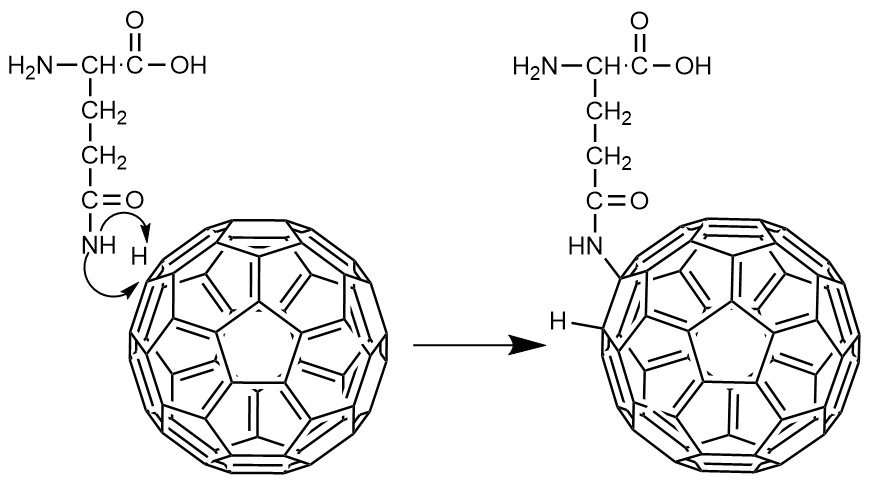
\includegraphics[width=0.7\textwidth,height=0.5\textwidth]{imagenes/Intro/Fullereno-glicina.png}
    \textbf{\caption{Reacción nucleofílica del C\textsubscript{60}(\textit{Gly})\textsubscript{4}.}
    \label{workin} }%Esto genera un numero a mi etiqueta
\end{figure}

\scriptsize{\cite{sharoyko2024modification}} Sharoyko, V. V. et al.,\emph{Journal of Molecular Liquids}, 2024. \\
\end{column}
\begin{column}{0.5\textwidth}
\begin{itemize}
    \item \textbf{Nucleófilo:} Grupo amino ($-\text{NH}_2$) de la glicina
    \item \textbf{Electrófilo:} Dobles enlaces ($\text{C}=\text{C}$) del fullereno $\text{C}_{60}$
    \item \textbf{Ataque:} Adición del par de electrones del nitrógeno al carbono
    \item \textbf{Formación:} Enlace covalente $\text{C}-\text{N}$
\end{itemize}
\end{column}
\end{columns}
\end{frame}












\section{Planteamiento del problema}
\begin{frame}{Planteamiento del problema}
\footnotesize \justifying
El dengue sigue siendo un problema de salud pública sin antivirales específicos realmente eficaces. La proteasa NS2B-NS3 del DENV2 es un blanco terapéutico clave y los fullerenos funcionalizados con aminoácidos son plataformas prometedoras al mejorar su solubilidad y estructura electrónica. Aún se desconoce cómo estas modificaciones afectan su interacción con NS2B-NS3, por lo que estudiarlas puede aportar bases para diseñar nuevos inhibidores contra el dengue.
\begin{center}
\fcolorbox{AzulOscuro!30}{GrisClaro}{
            \begin{minipage}{0.9\textwidth}
                \small
               ¿Cómo afecta la funcionalización de fullerenos con aminoácidos a su estructura electrónica y qué impacto tiene en su interacción con la proteína del dengue NS2B-NS3 correspondiente al serotipo DENV2?
            \end{minipage}
        }
  \end{center}


\begin{figure}
    \centering
    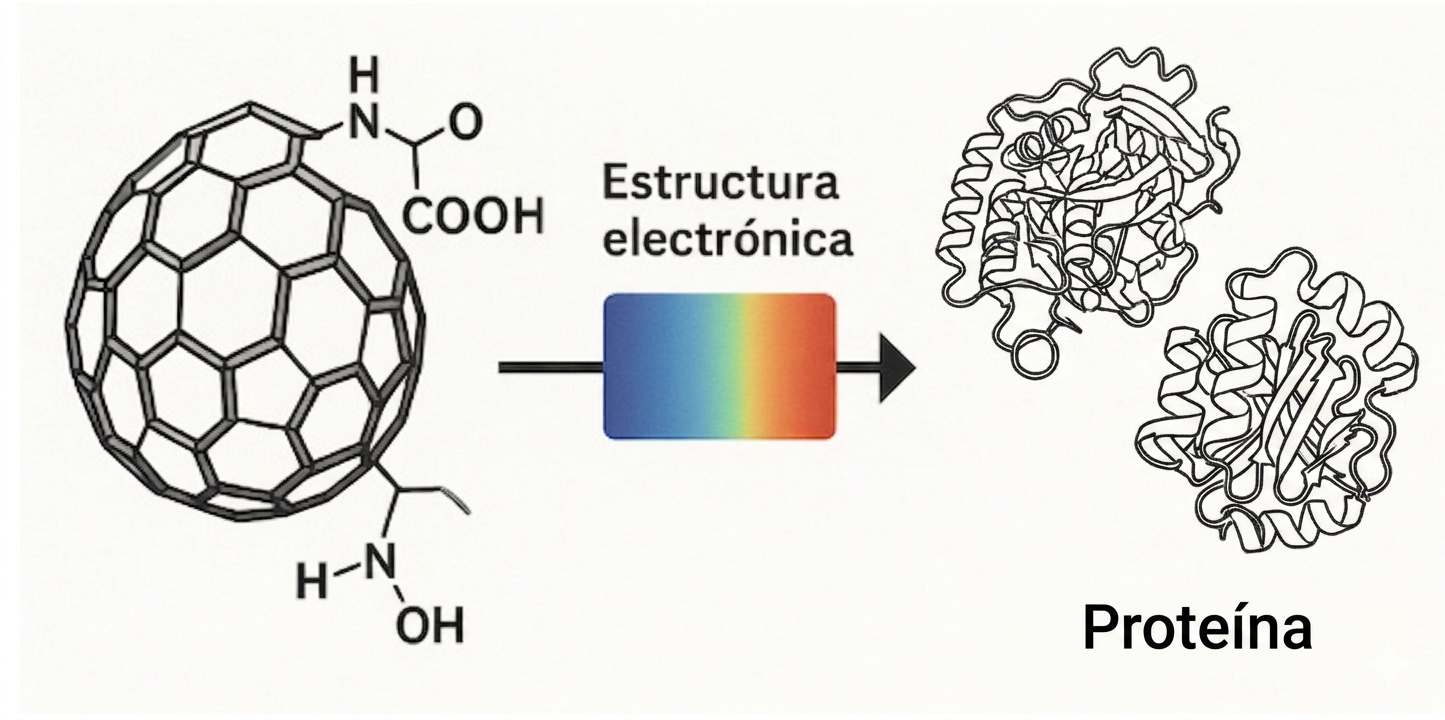
\includegraphics[width=0.4\textwidth,height=0.2\textwidth]{imagenes/Intro/planteamiento-1.png}

\end{figure}


\end{frame}

\section{Justificación}
\begin{frame}{Justificación}
\begin{center}
        \fcolorbox{AzulOscuro!30}{GrisClaro}{
            \begin{minipage}{0.9\textwidth}
                \small\centering
                Los fullerenos, conocidos por sus propiedades estructurales y electrónicas únicas, han captado el interés en aplicaciones biomédicas.
            \end{minipage}
        }
    \end{center}

    \vspace{0.3cm}

    % 2. FILAS CON TABLA (Más estable que TikZ para esta plantilla)
    \begin{table}
        \renewcommand{\arraystretch}{2.2} % Espaciado entre filas
        \centering
        \begin{tabular}{l c p{8.5cm}}
            
            % Fila 1
            \tikz[baseline=-0.5ex]\node[fill=AzulGris!20, draw=AzulGris, text=AzulOscuro, font=\bfseries\scriptsize, minimum width=2.5cm, minimum height=0.6cm, rounded corners=2pt]{Limitación}; & 
            \tikz[baseline=-0.5ex]\draw[AzulGris, thick, -{Stealth}] (0,0) -- (0.6,0); & 
            \footnotesize Su baja solubilidad en medios biológicos sigue siendo un obstáculo que restringe su potencial terapéutico. \\

            % Fila 2
            \tikz[baseline=-0.5ex]\node[fill=AzulGris!20, draw=AzulGris, text=AzulOscuro, font=\bfseries\scriptsize, minimum width=2.5cm, minimum height=0.6cm, rounded corners=2pt]{Solución}; & 
            \tikz[baseline=-0.5ex]\draw[AzulGris, thick, -{Stealth}] (0,0) -- (0.6,0); & 
            \footnotesize La funcionalización con aminoácidos como la glicina aumenta la solubilidad y mejora la afinidad. \\

            % Fila 3
            \tikz[baseline=-0.5ex]\node[fill=AzulGris!20, draw=AzulGris, text=AzulOscuro, font=\bfseries\scriptsize, minimum width=2.5cm, minimum height=0.6cm, rounded corners=2pt]{Herramientas}; & 
            \tikz[baseline=-0.5ex]\draw[AzulGris, thick, -{Stealth}] (0,0) -- (0.6,0); & 
            \footnotesize El uso de herramientas de acoplamiento y modelado molecular brinda una comprensión profunda. \\

            % Fila 4
            \tikz[baseline=-0.5ex]\node[fill=AzulGris!20, draw=AzulGris, text=AzulOscuro, font=\bfseries\scriptsize, minimum width=2.5cm, minimum height=0.6cm, rounded corners=2pt]{Impacto}; & 
            \tikz[baseline=-0.5ex]\draw[AzulGris, thick, -{Stealth}] (0,0) -- (0.6,0); & 
            \footnotesize Diseño racional de sistemas funcionalizados dirigidos a la proteína NS2B-NS3 del virus del dengue. \\
            
        \end{tabular}
    \end{table}
    \end{frame}

\section{Hipótesis}
\begin{frame}{Hipótesis}
\normalsize \justifying
La funcionalización de fullerenos con aminoácidos modifica su estructura electrónica, aumentando su solubilidad y reactividad, lo que mejora su interacción con biomoléculas y potencia su actividad para el acoplamiento con la diana terapéutica del serotipo 2 de NS2B-NS3 correspondiente al virus del Dengue.
\end{frame}

\section{Objetivos}
\begin{frame}{Objetivos}
    
    % --- Objetivo General ---
    \begin{center}
        \fcolorbox{AzulOscuro!30}{GrisClaro}{
            \begin{minipage}{0.9\textwidth}
                \small
                \textbf{Objetivo General} \vspace{2pt} \\
                Identificar las estructuras más estables del derivado C\textsubscript{60}(Gly)\textsubscript{4} y analizar su interacción con las proteínas NS2B-NS3 en conformación abierta y cerrada del DENV2.
            \end{minipage}
        }
    \end{center}

    \vspace{0.4cm}

    % --- Objetivos Particulares ---
    \textbf{Objetivos Particulares}
    
    \begin{enumerate}
        \footnotesize
        \item Evaluar los sitios de adición del aminoácido glicina en la estructura del fullereno C\textsubscript{60}.
        \item Valorar la solubilidad, reactividad química y capacidad de interacción del fullereno funcionalizado.
        \item Identificar los sitios de acoplamiento del C\textsubscript{60}(Gly)\textsubscript{4} con la proteína correspondiente al serotipo DENV2.
        \item Encontrar la relación entre la teoría y las tendencias experimentales, a partir de resultados teóricos.
    \end{enumerate}

\end{frame}
\section{Metodología}
%\begin{center}
%    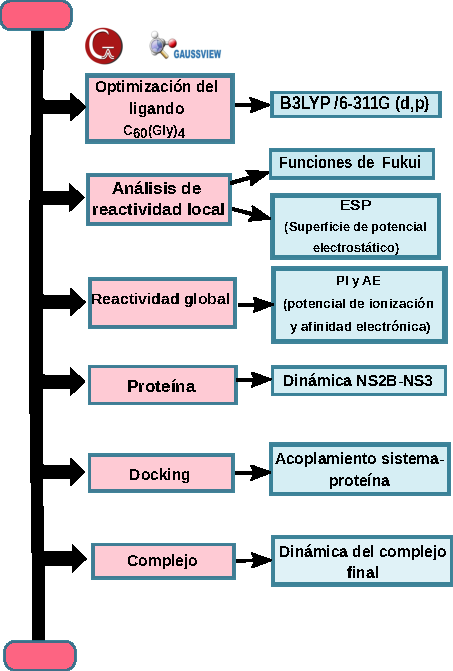
\includegraphics[width=0.5\textwidth]{imagenes/metodologia/metodologiatesis-3.pdf}\\[0.4em]
%    \textbf{Diagrama de la metodología.}
%\end{center}
%----------------------------------------------------------------------------------------------
\section{Resultados y Discusiones}

\begin{frame}{Comparación Energética de los Complejos  C\textsubscript{60}(\textit{Gly})}
\begin{columns}
\begin{column}{0.45\textwidth}
%1-----------------------------

\begin{table}[H]
\centering
\caption{Energías de formación de los isómeros del complejo C\textsubscript{60}(\textit{Gly}).}
\label{tab:fukui_gly1}
\resizebox{\linewidth}{!}{%
\begin{tabular}{ccc}
\toprule
\textbf{Sistema} & \textbf{Carbonos} & \textbf{Energía kcal/mol} \\
\midrule
C\textsubscript{60}(\textit{Gly}) -- a & C59, C43 & 37.268 \\
C\textsubscript{60}(\textit{Gly}) -- b & C59, C58 & 6.303 \\
\textcolor{red}{C\textsubscript{60}(\textit{Gly}) -- c} & \textcolor{red}{C59, C11} & \textcolor{red}{0} \\
C\textsubscript{60}(\textit{Gly}) -- d & C59, C10 & 17.075 \\
C\textsubscript{60}(\textit{Gly}) -- e & C59, C50 & 46.752 \\
C\textsubscript{60}(\textit{Gly}) -- f & C59, C51 & 28.839 \\
\bottomrule
\end{tabular}%
}
\end{table}

\end{column}

\begin{column}{0.55\textwidth}

\begin{figure}[h]
    \centering
    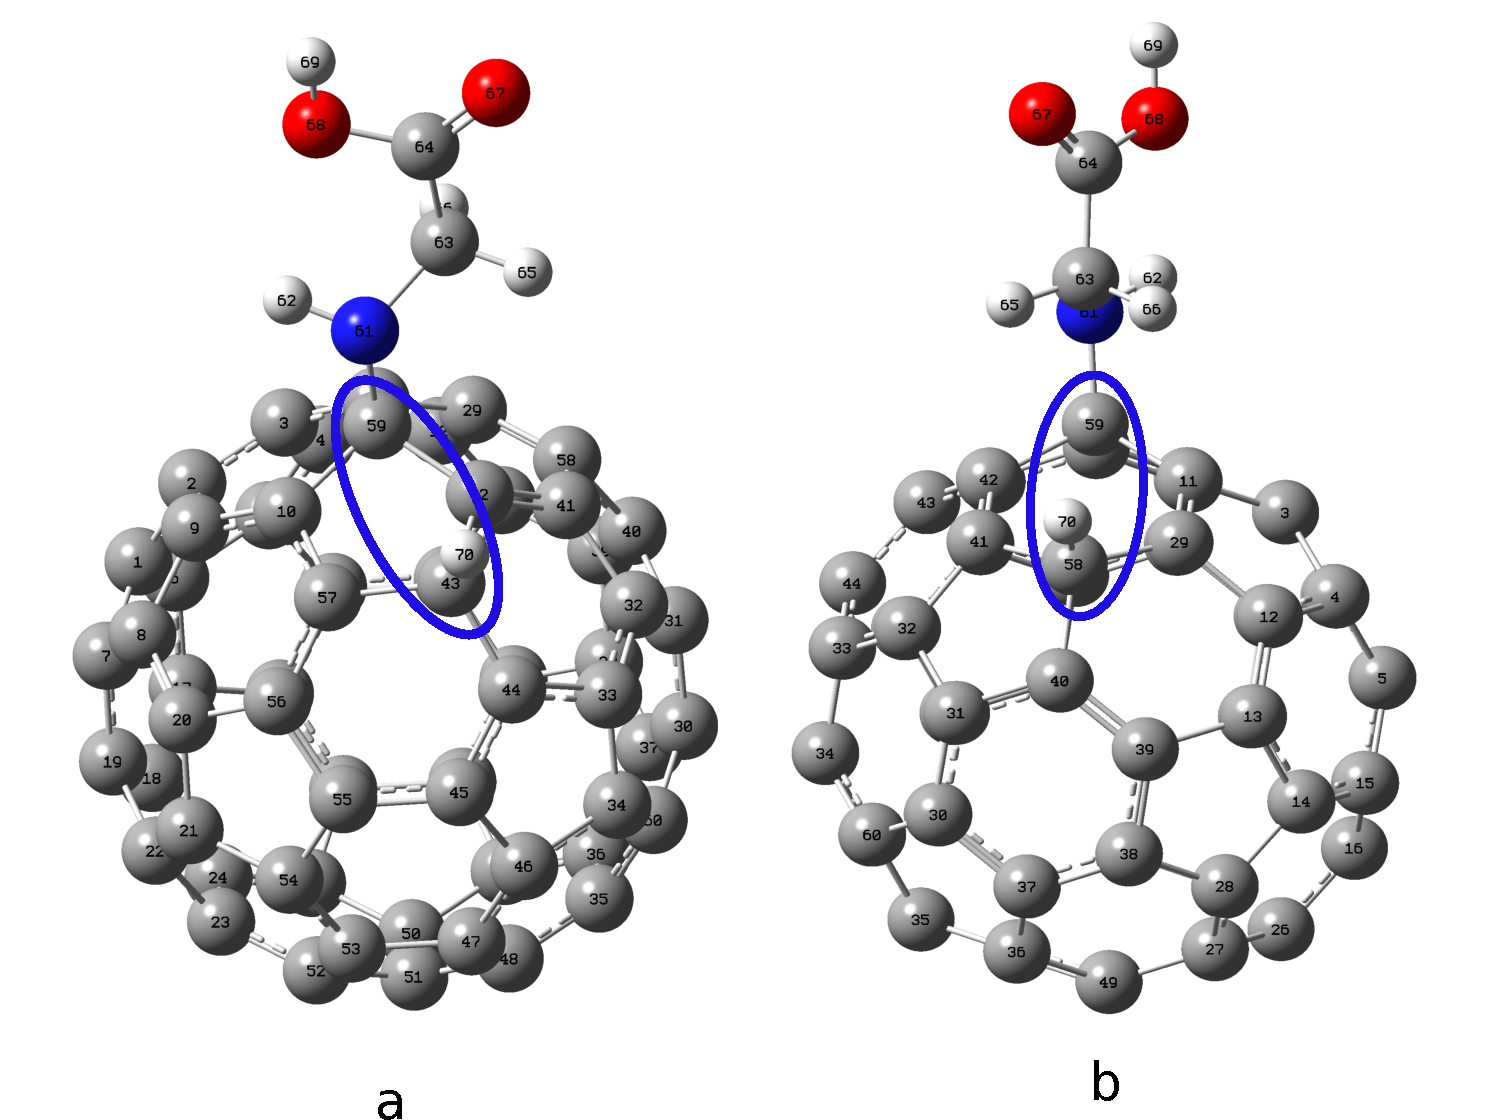
\includegraphics[width=1\textwidth,height=0.8\textwidth]{imagenes/Resultados/fukui-1.pdf}
      \caption{\textbf{Posiciones de los carbonos correspondientes a los sistemas $a$ y $b$.}}
   
\end{figure}
\end{column}
\end{columns}
\end{frame}

\begin{frame}{Comparación Energética de los Complejos  C\textsubscript{60}(\textit{Gly}) }
\begin{columns}
\begin{column}{0.5\textwidth}
%-----------------------------
\begin{table}[H]
    \centering
    \vspace{-0.2cm}
    \label{tab:gibbs_thermo_conv}
      \footnotesize
   \begin{figure}[h]
    \centering
    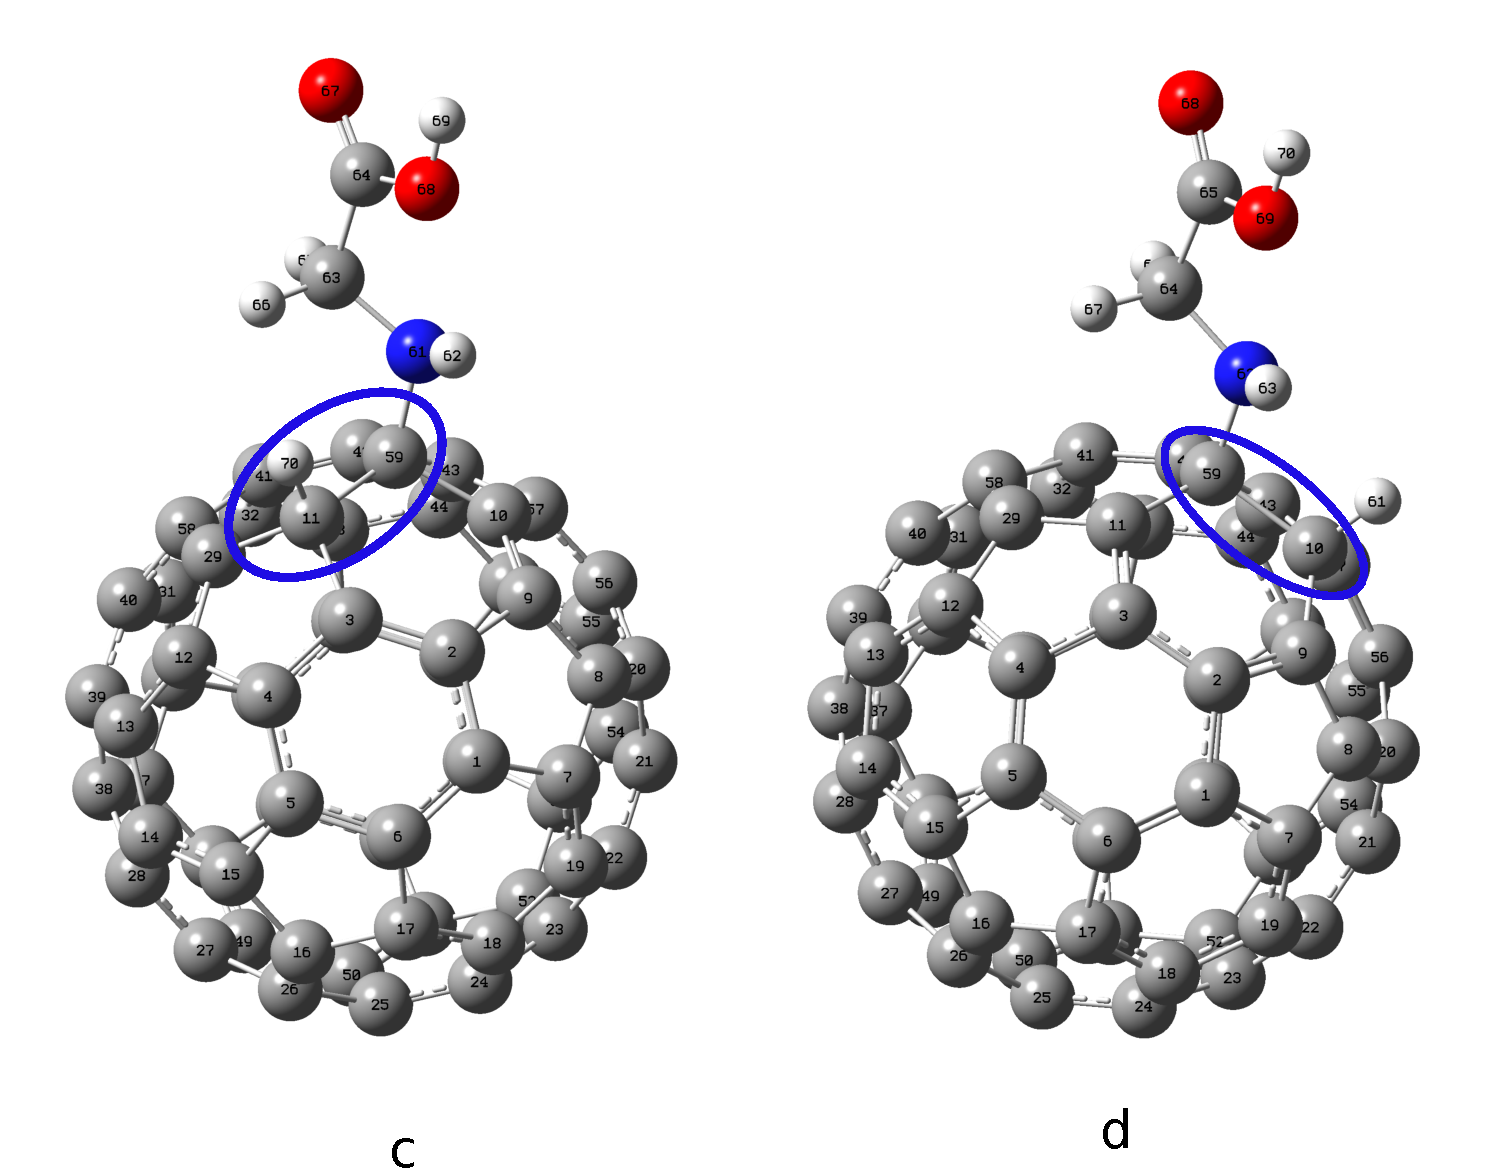
\includegraphics[width=1\textwidth,height=0.9\textwidth]{imagenes/Resultados/fukui-2.pdf}
      \caption{\textbf{Posiciones de los carbonos correspondientes a los sistemas $c$ y $d$.}}
\end{figure}
\end{table}
\end{column}

\begin{column}{0.5\textwidth}
\vspace{-1cm}
\begin{figure}[h]
    \centering
    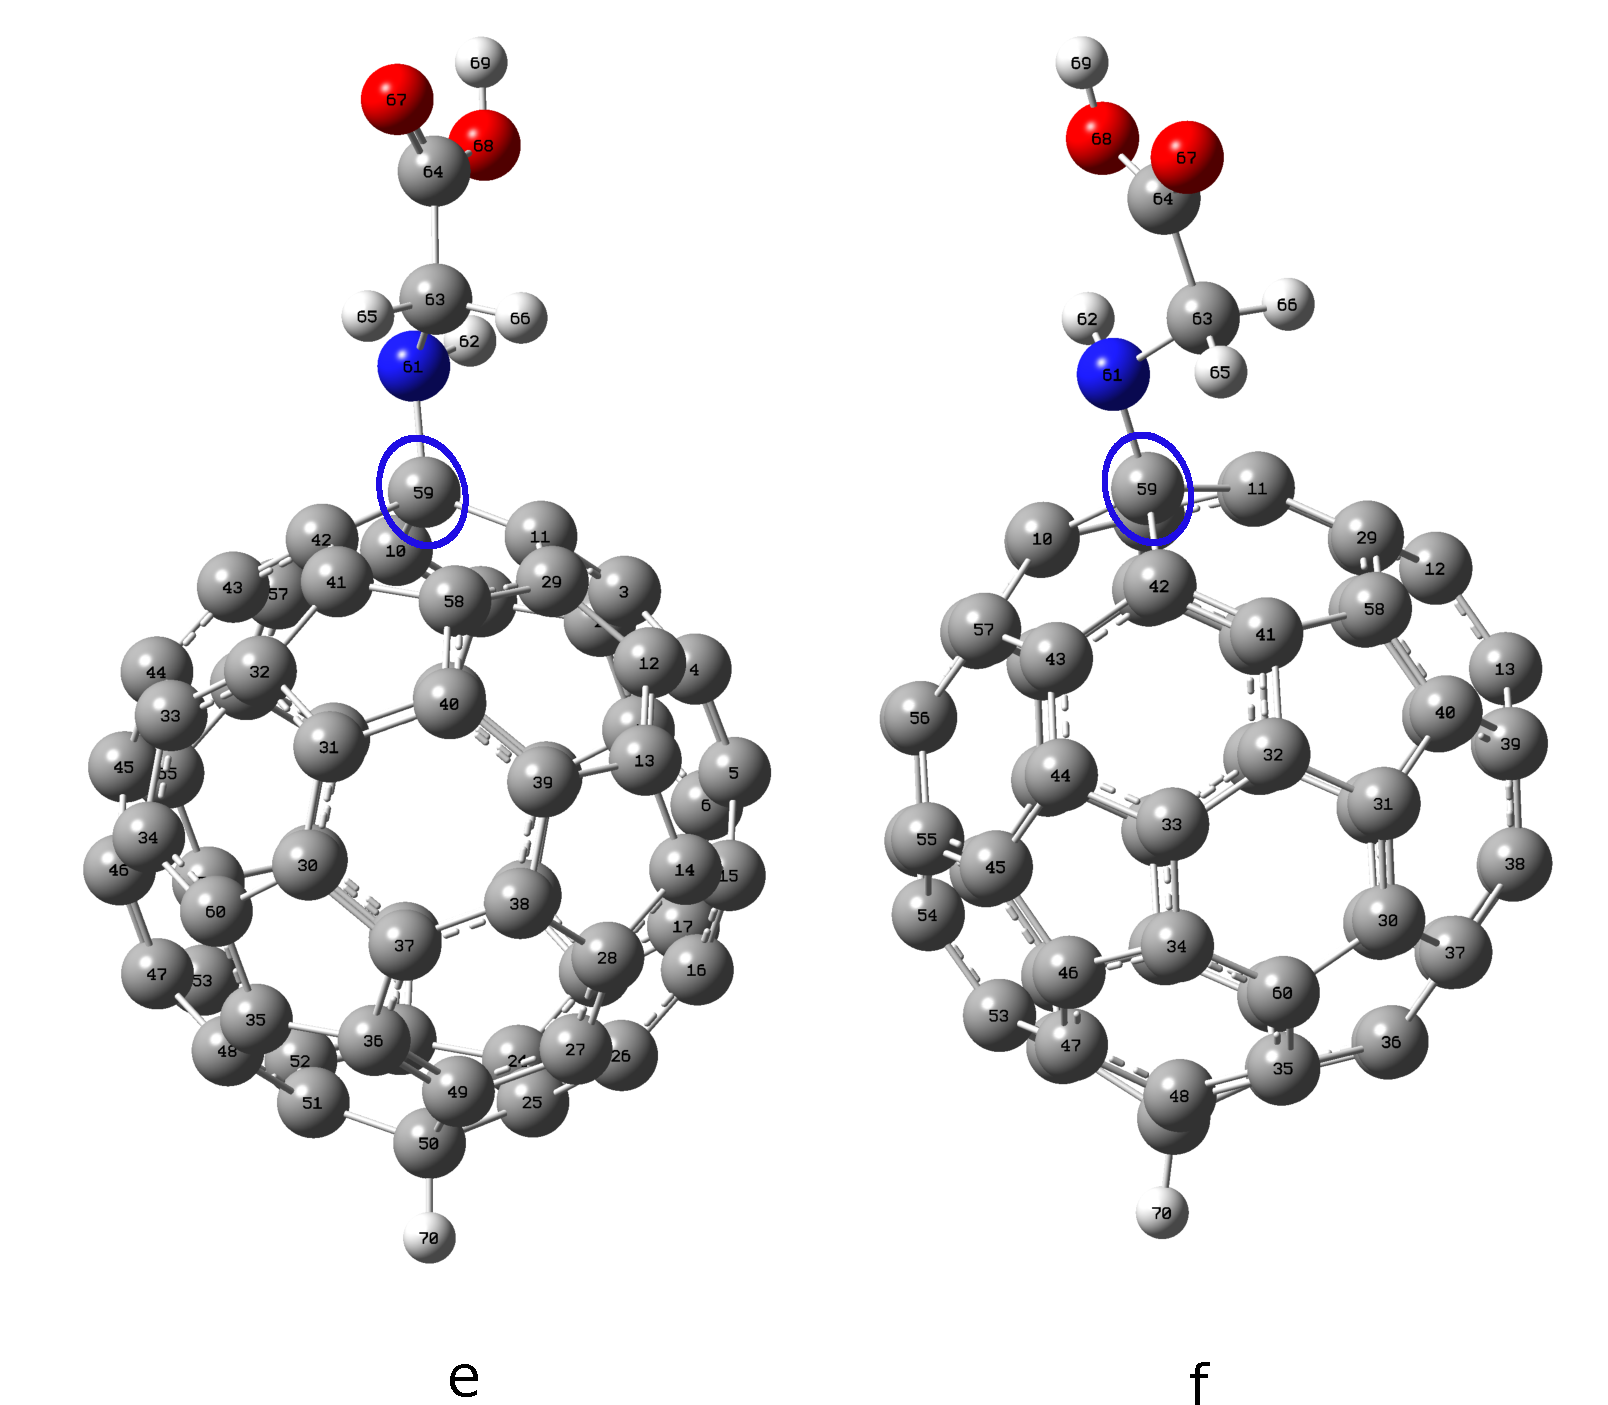
\includegraphics[width=1\textwidth,height=0.9\textwidth]{imagenes/Resultados/fukui-3.pdf}
      \caption{\textbf{Posiciones de los carbonos correspondientes a los sistemas $e$ y $f$.}}
   
\end{figure}
\end{column}
\end{columns}
\end{frame}
%2---------------------------------------------------------------
\begin{frame}{Comparación Energética de los Complejos C\textsubscript{60}(\textit{Gly})\textsubscript{2}}
\begin{columns}
\begin{column}{0.5\textwidth}
%-----------------------------
\vspace*{-1cm}
\begin{table}[H]
\centering
\caption{Cálculo de energías para la adición múltiple de glicina en C\textsubscript{60} basada en índices de reactividad de Fukui C\textsubscript{60}(\textit{Gly})\textsubscript{2}.}
\label{tab:fukui_gly2}
\resizebox{\linewidth}{!}{%
\begin{tabular}{ccc}
\toprule
\textbf{Sistema con C\textsubscript{60}(\textit{Gly})\textsubscript{2}} & \textbf{Carbonos} & \textbf{Energía kcal/mol} \\
\midrule
C\textsubscript{60}(\textit{Gly})\textsubscript{2} -- a & C31, C30 & 0.696 \\
C\textsubscript{60}(\textit{Gly})\textsubscript{2} -- b & C07, C19 & 0.789 \\
C\textsubscript{60}(\textit{Gly})\textsubscript{2} -- c & C28, C27 & 0.850 \\
\textcolor{red}{C\textsubscript{60}(\textit{Gly})\textsubscript{2} -- d} & \textcolor{red}{C54, C53} & \textcolor{red}{0} \\
\bottomrule
\end{tabular}%
}
\end{table}





\end{column}

\begin{column}{0.5\textwidth}
\vspace*{-1cm}
\begin{figure}[h]
    \centering
    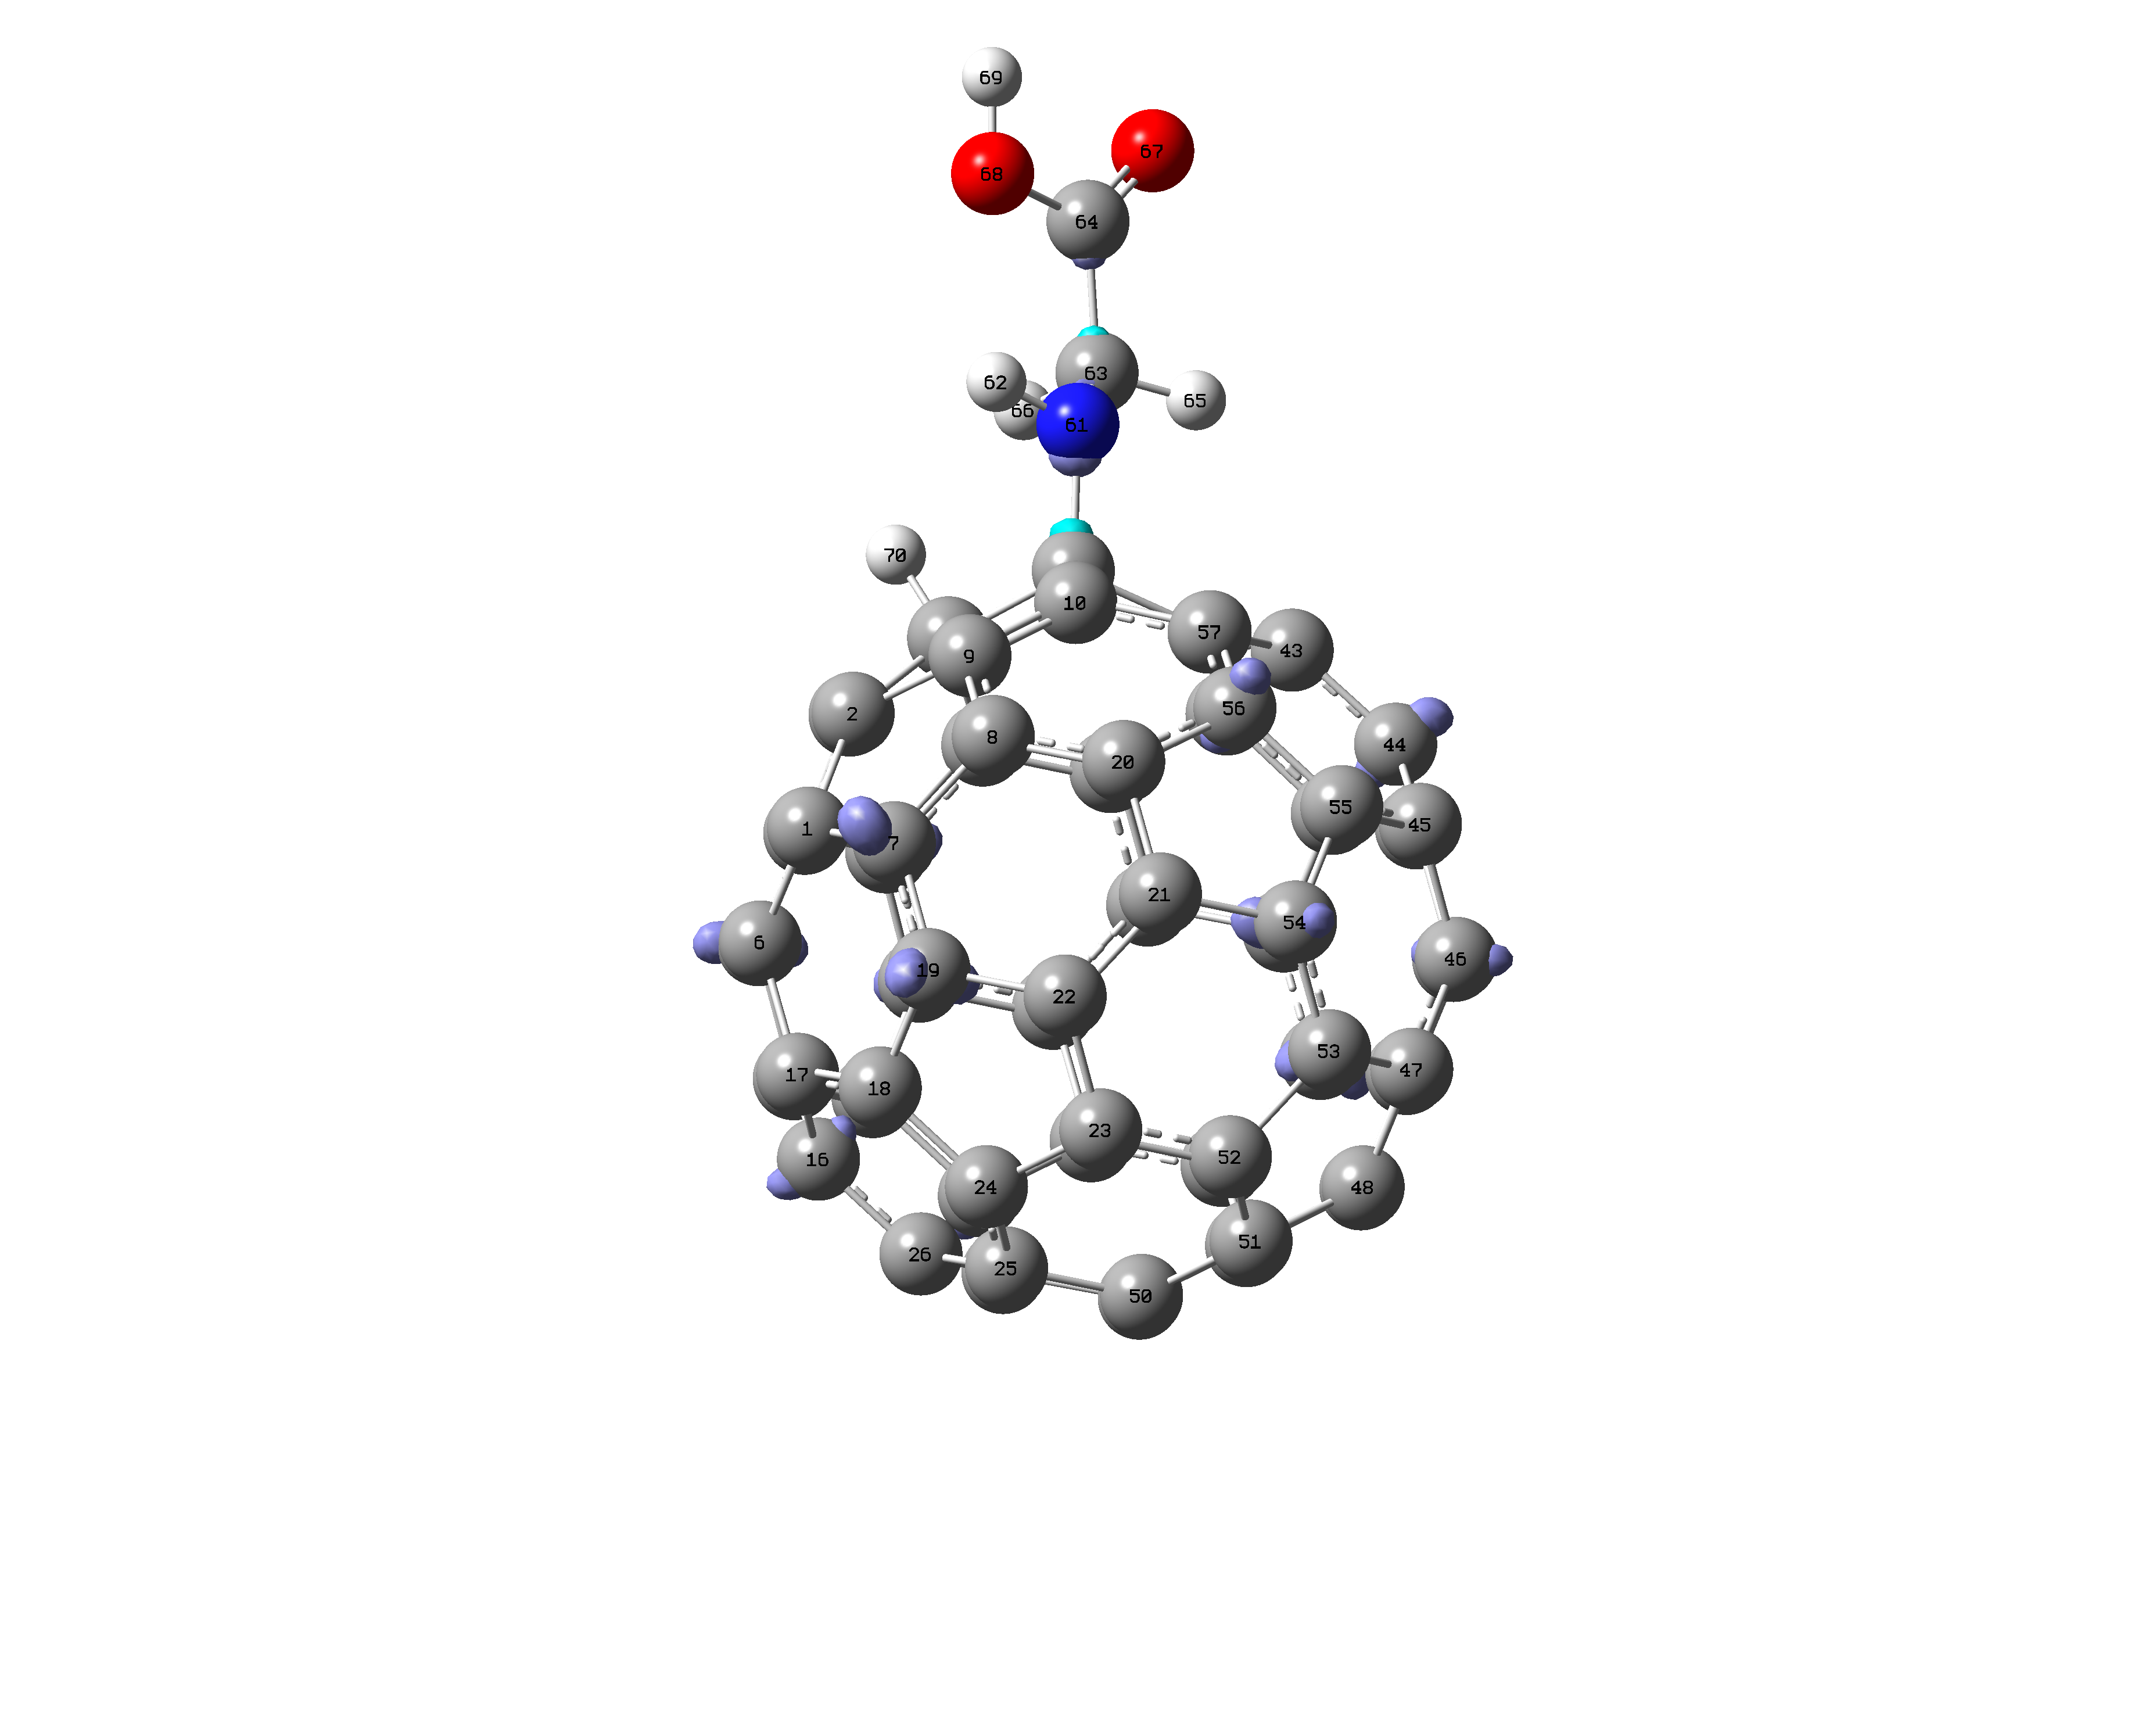
\includegraphics[width=1.1\textwidth,height=1.0\textwidth]{imagenes/Resultados/C60-gli-1-prueba-4.png}
     \vspace*{-2cm}
     \justifying
      \caption{\textbf{Posiciones de los carbonos correspondientes al sistemas $d$.}}
   
\end{figure}
\end{column}
\end{columns}
\end{frame}
%3------------------------------------------------------------------------
\begin{frame}{Comparación Energética de los Complejos  C\textsubscript{60}(\textit{Gly})\textsubscript{3}}
\begin{columns}
\begin{column}{0.4\textwidth}
%-----------------------------
\vspace*{-2cm}
\begin{table}[H]
\centering
\caption{Cálculo de energías para la adición múltiple de glicina en C\textsubscript{60} basada en índices de reactividad de Fukui C\textsubscript{60}(\textit{Gly})\textsubscript{3}.}
\label{tab:fukui_gly3}
\resizebox{\linewidth}{!}{%
\begin{tabular}{ccc}
\toprule
\textbf{Sistema con C\textsubscript{60}(\textit{Gly})\textsubscript{3}} & \textbf{Carbonos} & \textbf{Energía kcal/mol} \\
\midrule
\textcolor{red}{C\textsubscript{60}(\textit{Gly})\textsubscript{3} -- a} & \textcolor{red}{C28, C27} & \textcolor{red}{0} \\
C\textsubscript{60}(\textit{Gly})\textsubscript{3} -- b & C35, C48 & 3.935 \\
C\textsubscript{60}(\textit{Gly})\textsubscript{3} -- c & C30, C31 & 1.142 \\
C\textsubscript{60}(\textit{Gly})\textsubscript{3} -- d & C17, C18 & 1.208 \\
\bottomrule
\end{tabular}%
}
\end{table}

\end{column}

\begin{column}{0.6\textwidth}
\vspace*{-0.5cm}
\begin{figure}[h]
    \centering
    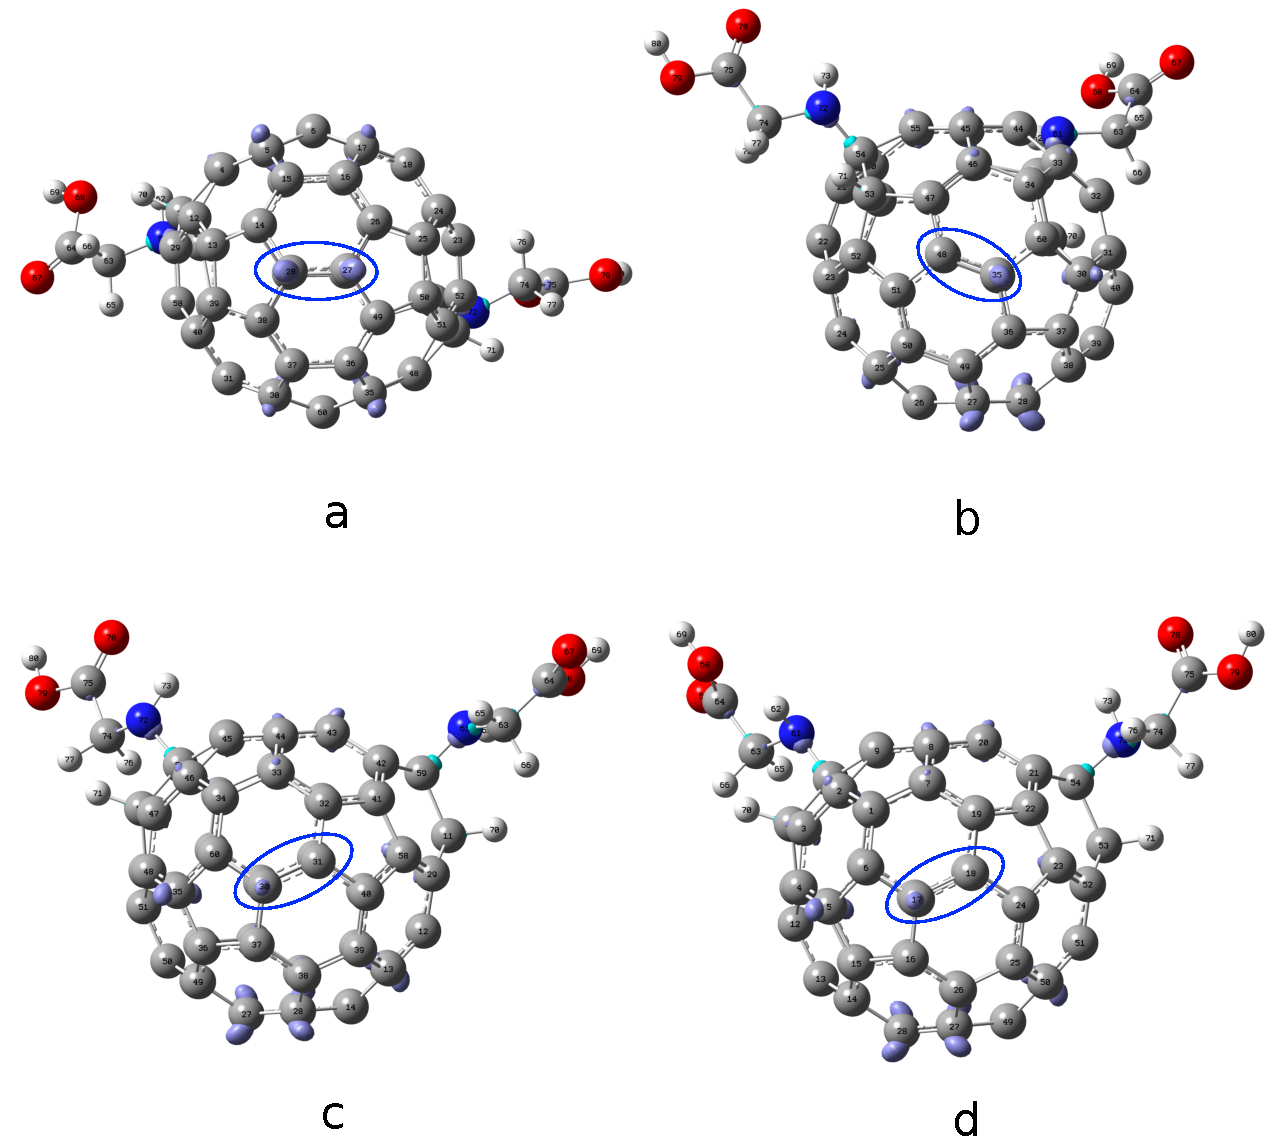
\includegraphics[width=0.9\textwidth,height=0.8\textwidth]{imagenes/Resultados/fukui-3-nuevo.pdf}
   
      \caption{\textbf{Posiciones de los carbonos correspondientes a los sistemas $a$, $b$, $c$ y $d$.}}
   
\end{figure}
\end{column}
\end{columns}
\end{frame}
%4-----------------------------------------------------------------------
\begin{frame}{Comparación energética de los complejos  C\textsubscript{60}(\textit{Gly})\textsubscript{4}}
\begin{columns}
\begin{column}{0.4\textwidth}
%-----------------------------
\vspace*{-2cm}
\begin{table}[H]
\centering
\caption{Cálculo de energías para la adición múltiple de glicina en C\textsubscript{60} basada en índices de reactividad de Fukui C\textsubscript{60}(\textit{Gly})\textsubscript{4}.}
\label{tab:gibbs_thermo_conv}
\resizebox{\linewidth}{!}{%
\begin{tabular}{ccc}
\toprule
\textbf{Sistema con C\textsubscript{60}(\textit{Gly})\textsubscript{4}} & \textbf{Carbonos} & \textbf{Energía kcal/mol} \\
\midrule
C\textsubscript{60}(\textit{Gly})\textsubscript{4} -- a & C52, C23 & 0.676 \\
\textcolor{red}{C\textsubscript{60}(\textit{Gly})\textsubscript{4} -- b} & \textcolor{red}{C29, C58} & \textcolor{red}{0} \\
C\textsubscript{60}(\textit{Gly})\textsubscript{4} -- c & C49, C36 & 0.640 \\
C\textsubscript{60}(\textit{Gly})\textsubscript{4} -- d & C14, C15 & 2.180 \\
\bottomrule
\end{tabular}%
}
\end{table}
\end{column}

\begin{column}{0.6\textwidth}
\vspace*{-0.75cm}
\begin{figure}[h]
    \centering
    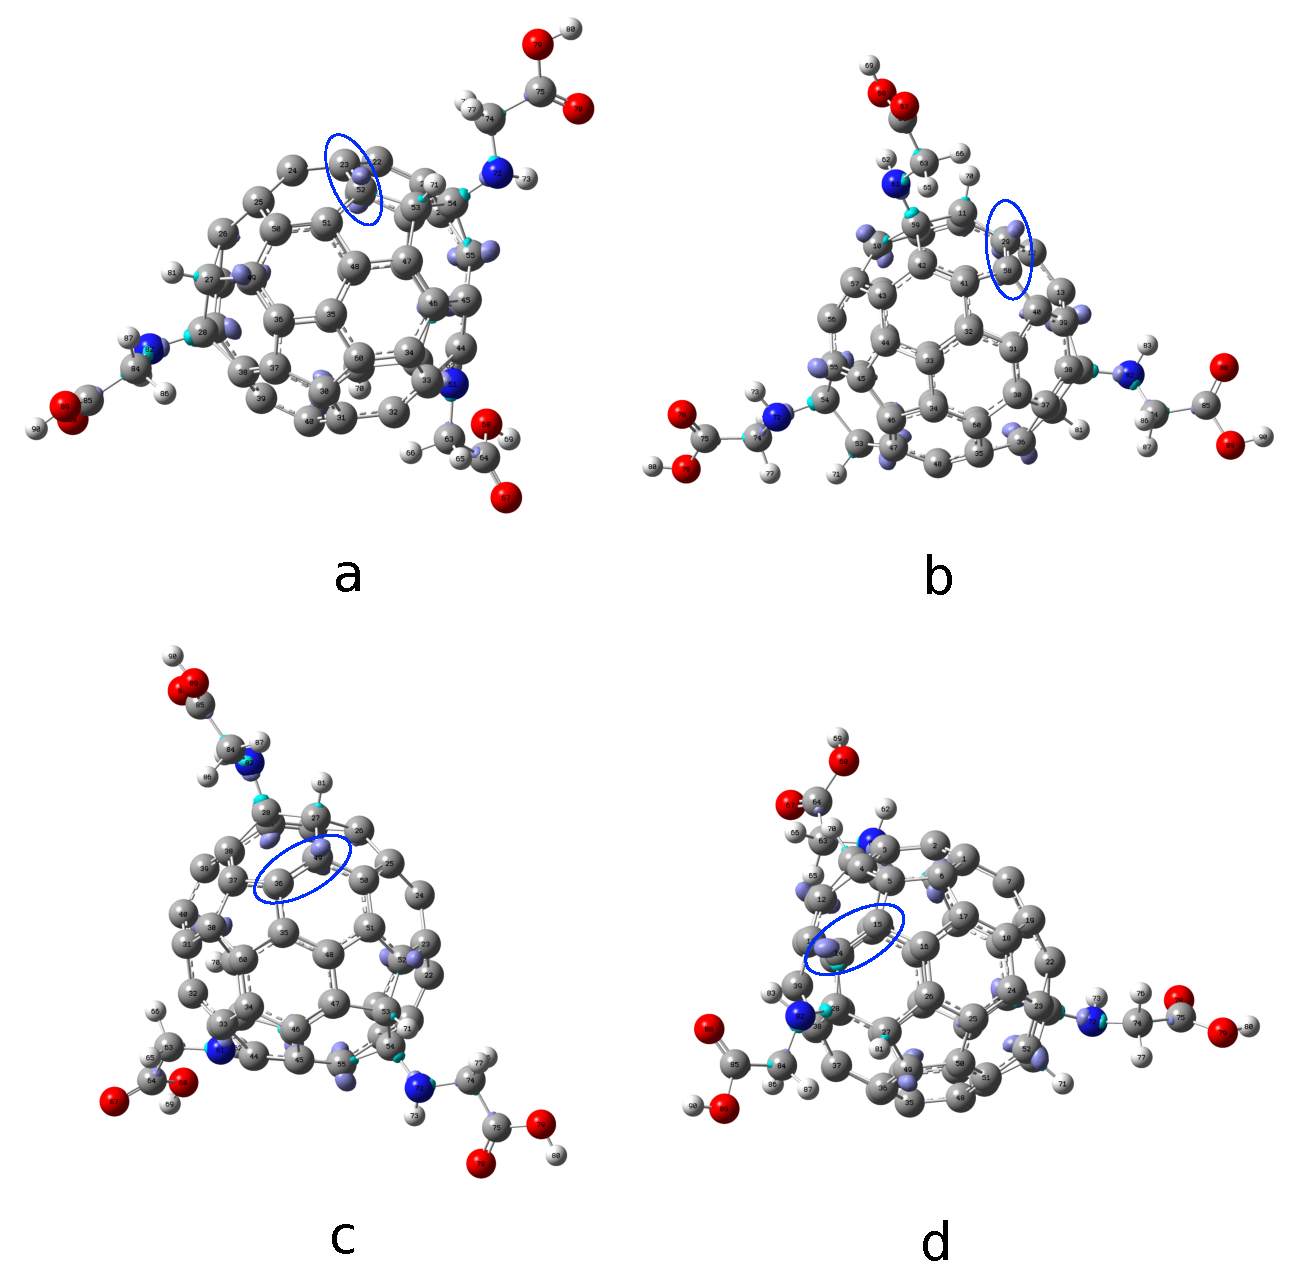
\includegraphics[width=0.9\textwidth,height=0.8\textwidth]{imagenes/Resultados/fukui-4-nuevo.pdf}
      \caption{\textbf{Posiciones de los carbonos correspondientes a los sistemas $a$, $b$, $c$ y $d$.}}
   
\end{figure}
\end{column}
\end{columns}
\end{frame}
%----------------------------------------------------------------------
\begin{frame}{Estructura final de C\textsubscript{60}(\textit{Gly})\textsubscript{4}}
\vspace*{-0.3cm}
\begin{figure}[h]
    \centering
    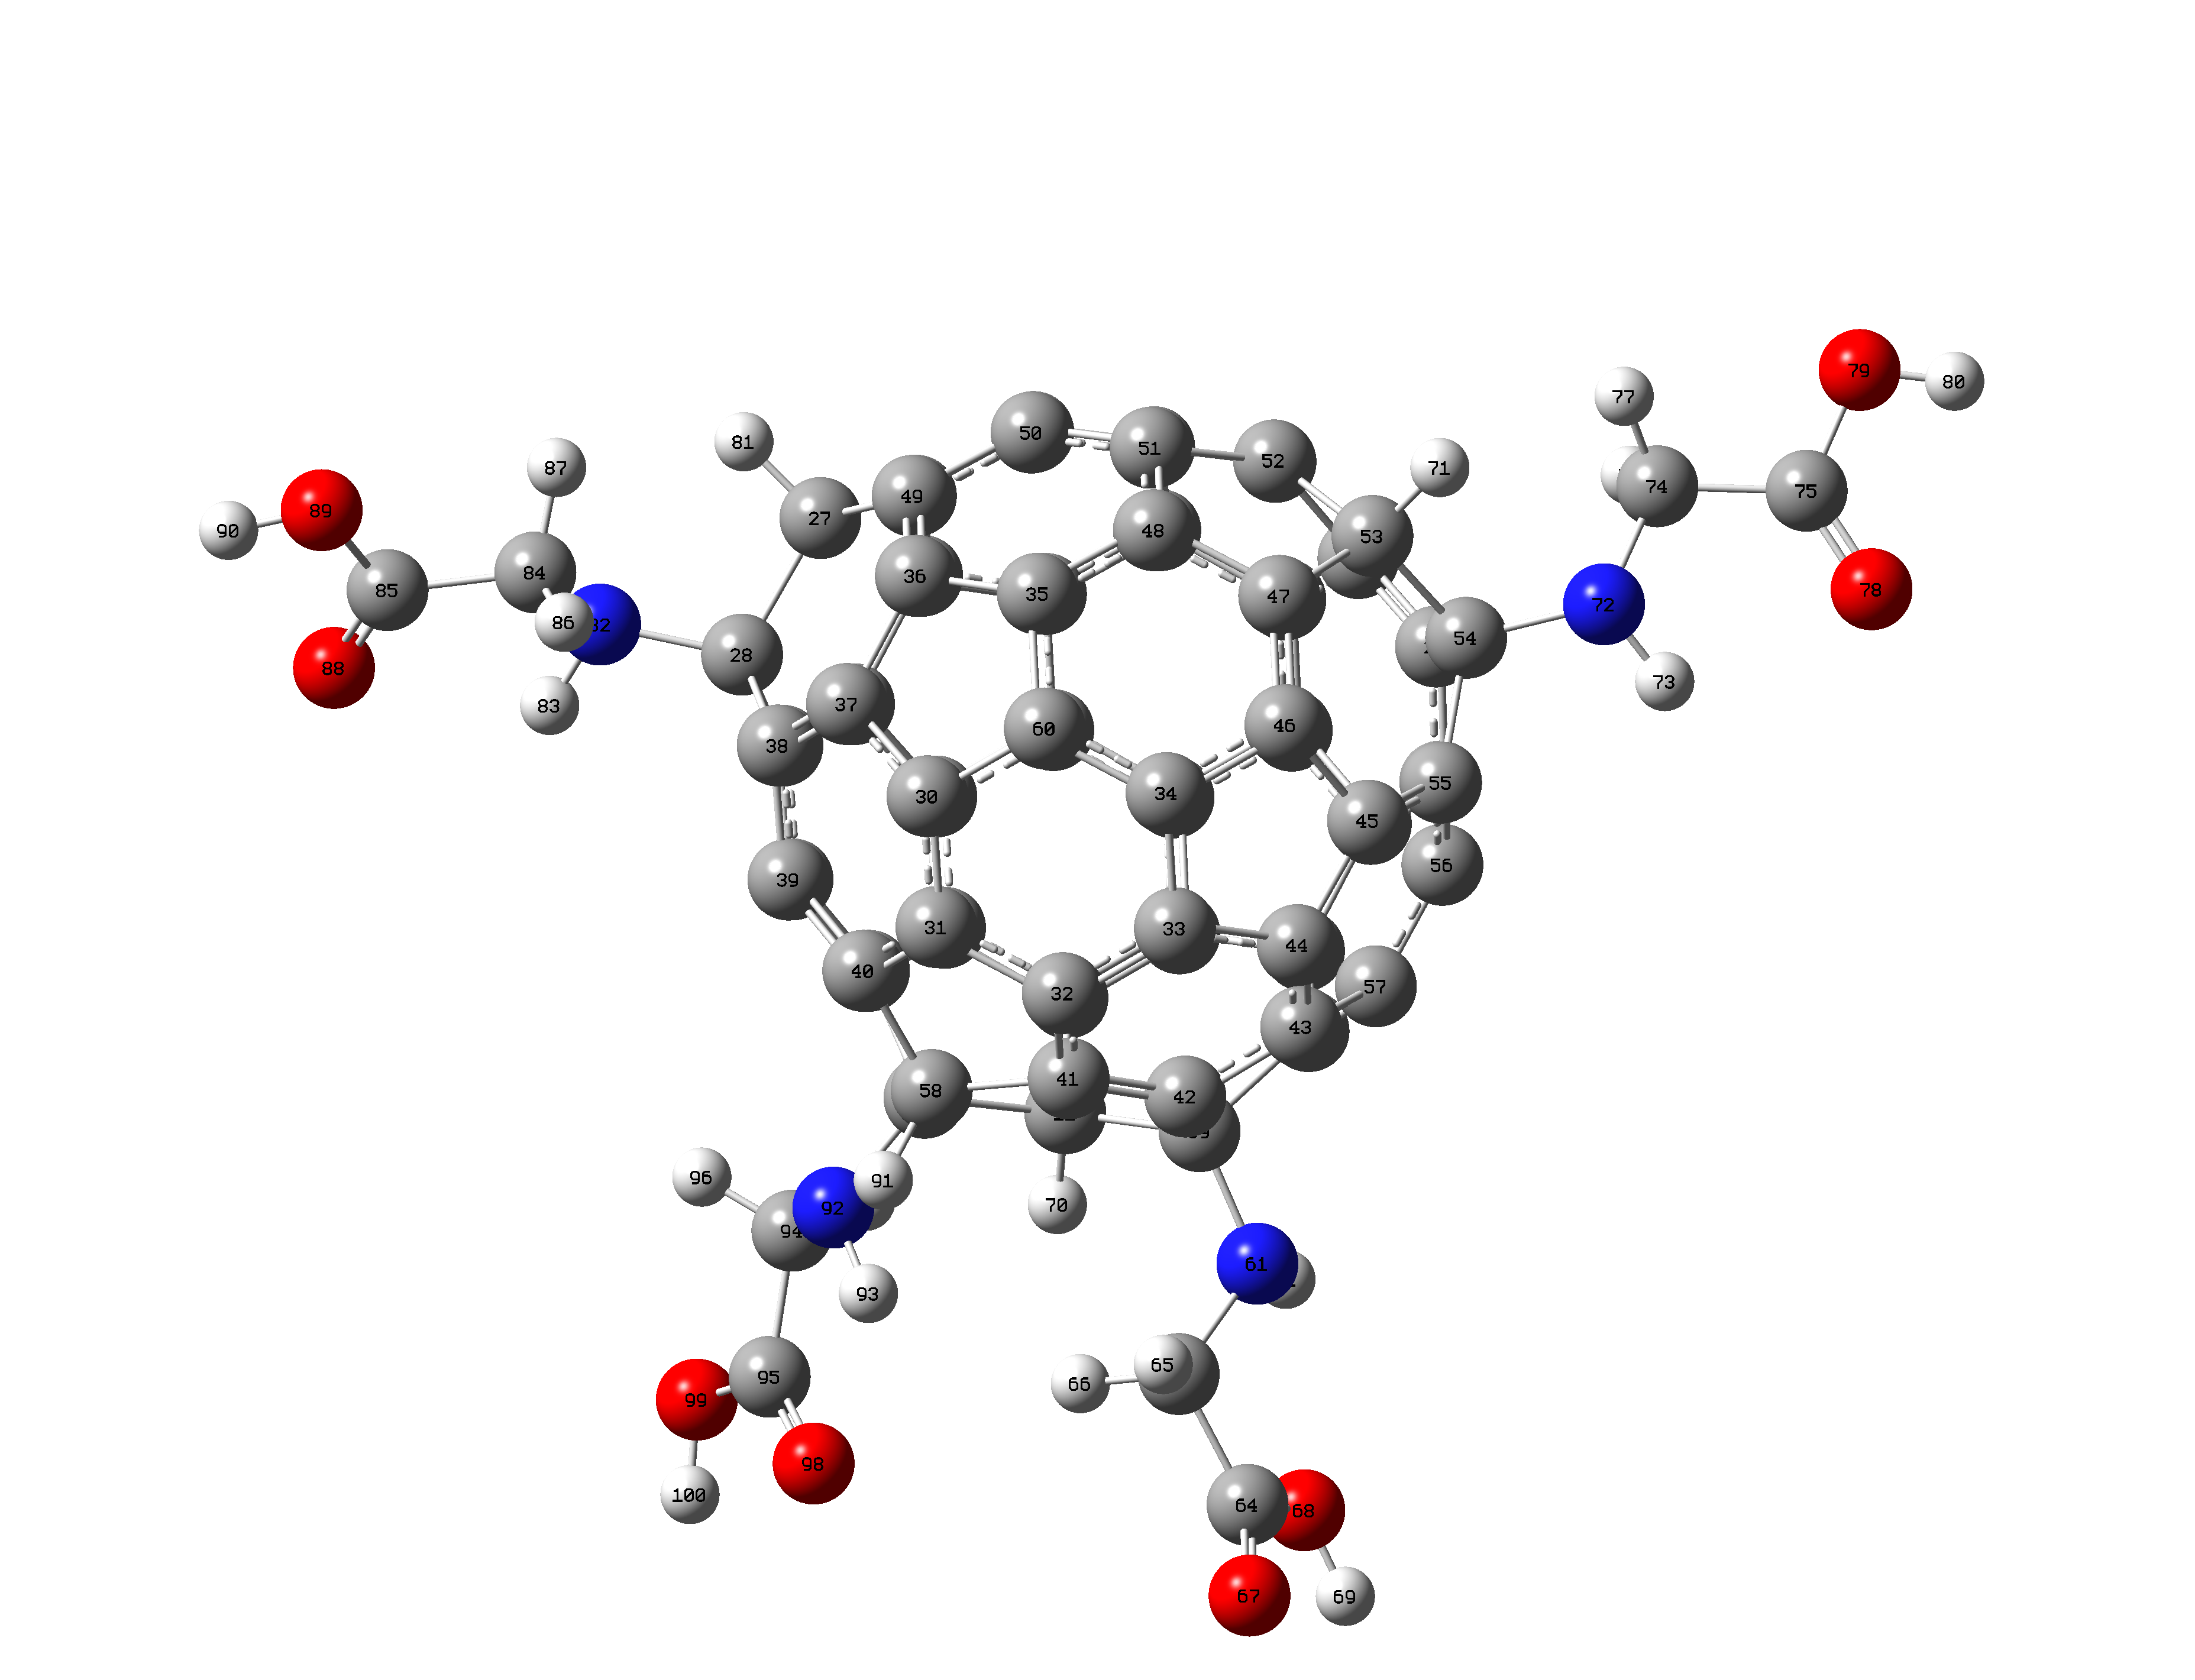
\includegraphics[width=0.5\textwidth,height=0.4\textwidth]{imagenes/Resultados/prueba-final.png}
      \caption{\textbf{Sistema completo de  C\textsubscript{60}(\textit{Gly})\textsubscript{4}.}}
   
\end{figure}
\end{frame}

%---------------------------------------------------------------
\begin{frame}{Funciones de Fukui: Reactividad electrofílica, nucleofílica y radicalaria}
\begin{figure}[h]
    \centering
    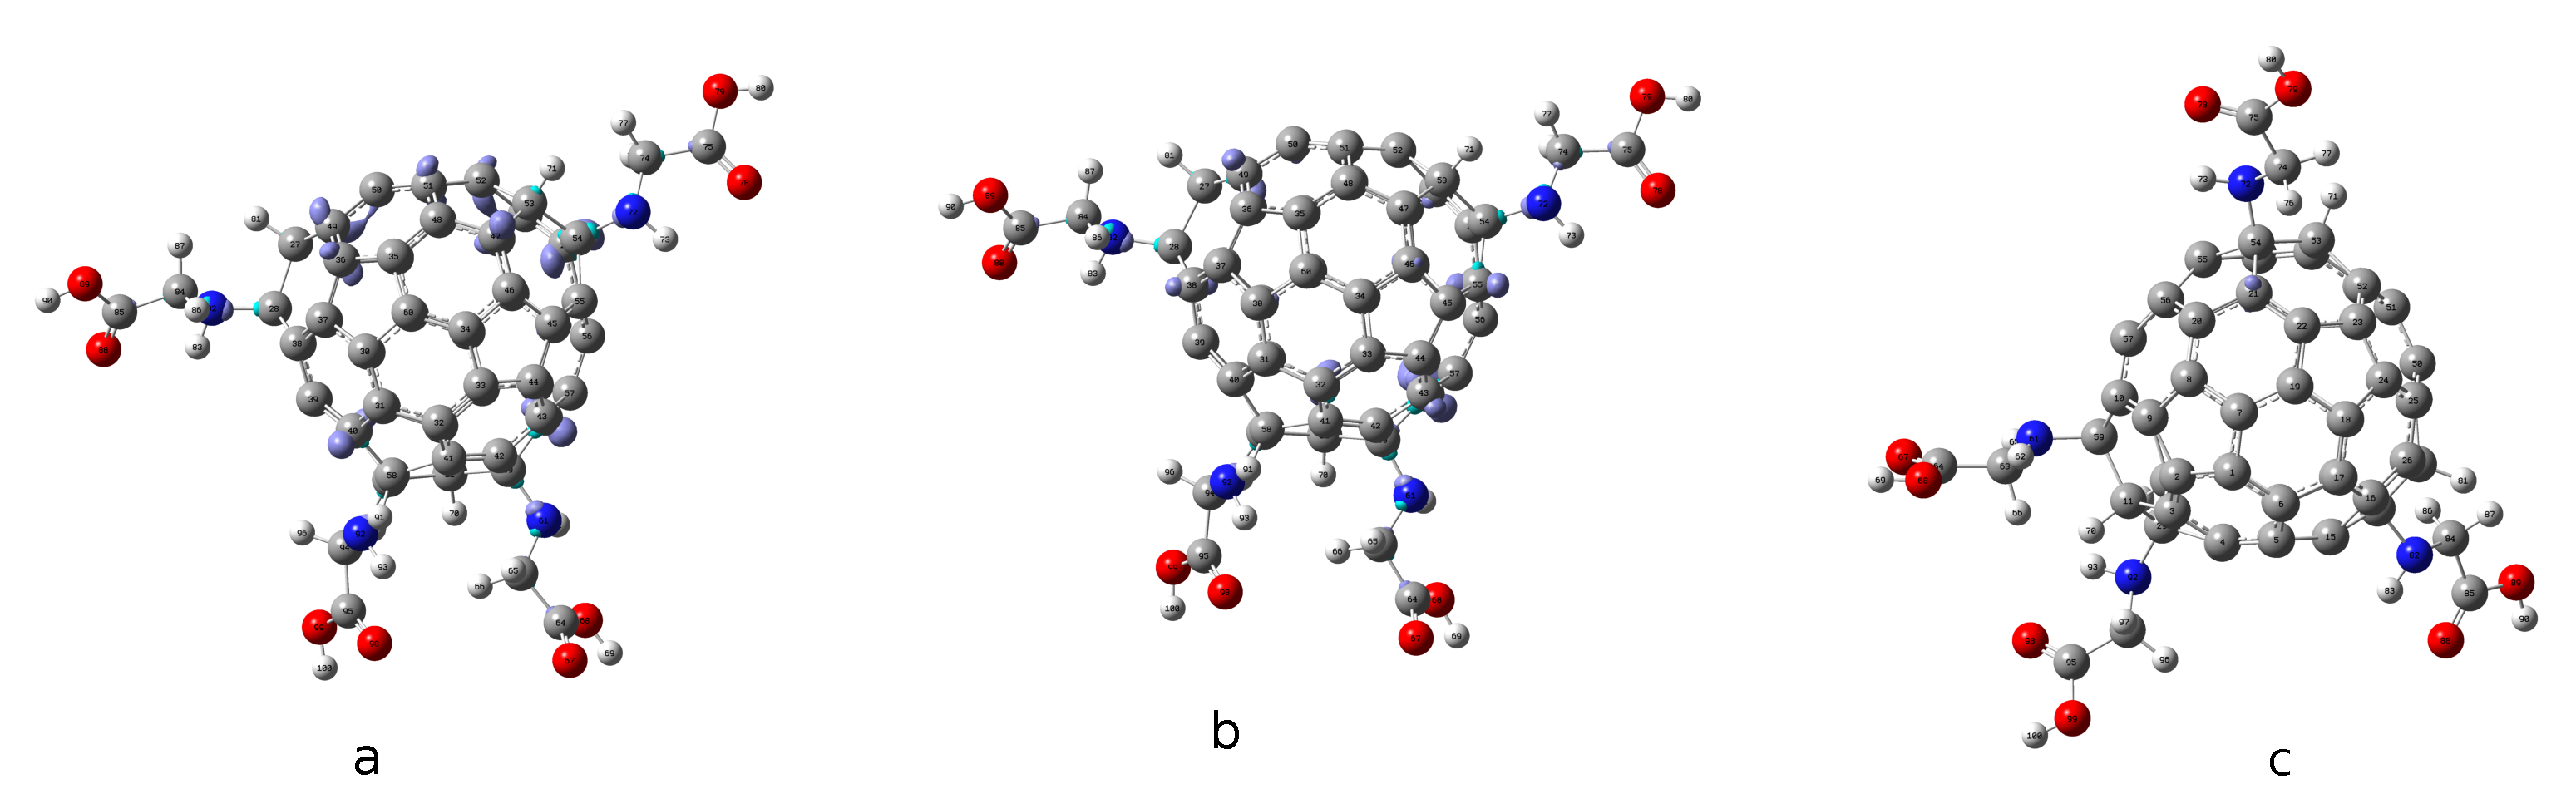
\includegraphics[width=1.0\textwidth,height=0.35\textwidth]{imagenes/Resultados/radicalaria.pdf}
      \caption{\textbf{Análisis de reactividad local: Funciones de Fukui del  C\textsubscript{60}(\textit{Gly})\textsubscript{4}:La figura ``\textbf{a}'' representa la función de Fukui nucleofílica, ``\textbf{b} '' la función de Fukui electrofílica y el inciso ``\textbf{c}'' corresponde a la función de Fukui radicalaria}.}
\end{figure}
\end{frame}

%----------------------------------------------------------------------


%-------------------------------------------------------------------------
\begin{frame}{Potencial electrostático promedio del  C\textsubscript{60}(\textit{Gly})\textsubscript{4}}
\begin{columns}
\begin{column}{0.3\textwidth}
\vspace*{-1.5cm}

\begin{table}[H]
\centering
\caption{Valores de potencial electrostático para cada sistema de C\textsubscript{60}(Gly).}
\label{tab:potencial_electrostatico}
\resizebox{\linewidth}{!}{%
\begin{tabular}{cc} % Definimos 2 columnas
\toprule
\textbf{Fragmento} & \textbf{Energía kcal/mol} \\
\midrule
Fullereno & 1.465 \\
(Gly -- 1) & 0.975 \\
(Gly -- 2) & 2.289 \\
(Gly -- 3) & 2.556 \\
(Gly -- 4) & 6.024 \\
\midrule % Una línea delgada para separar el promedio
\textbf{Promedio global por átomo} & \textbf{2.004} \\
\bottomrule
\end{tabular}%
}
\end{table}

\end{column}


\begin{column}{0.7\textwidth}
\begin{figure}[h]
    \centering
    \includegraphics[width=0.9\textwidth,height=0.5\textwidth]{imagenes/Resultados/figure_1.png}
      \caption{\textbf{Potencial electrostático promedio para  C\textsubscript{60}(\textit{Gly})\textsubscript{4}.}}
\end{figure}

\end{column}
\end{columns}
\end{frame}
%------------------------------------------------------------------------------------------



\begin{frame}{Mapa de potencial elesctrostático del sistema C\textsubscript{60}(\textit{Gly})\textsubscript{4}}
\begin{figure}[h]
    \centering
    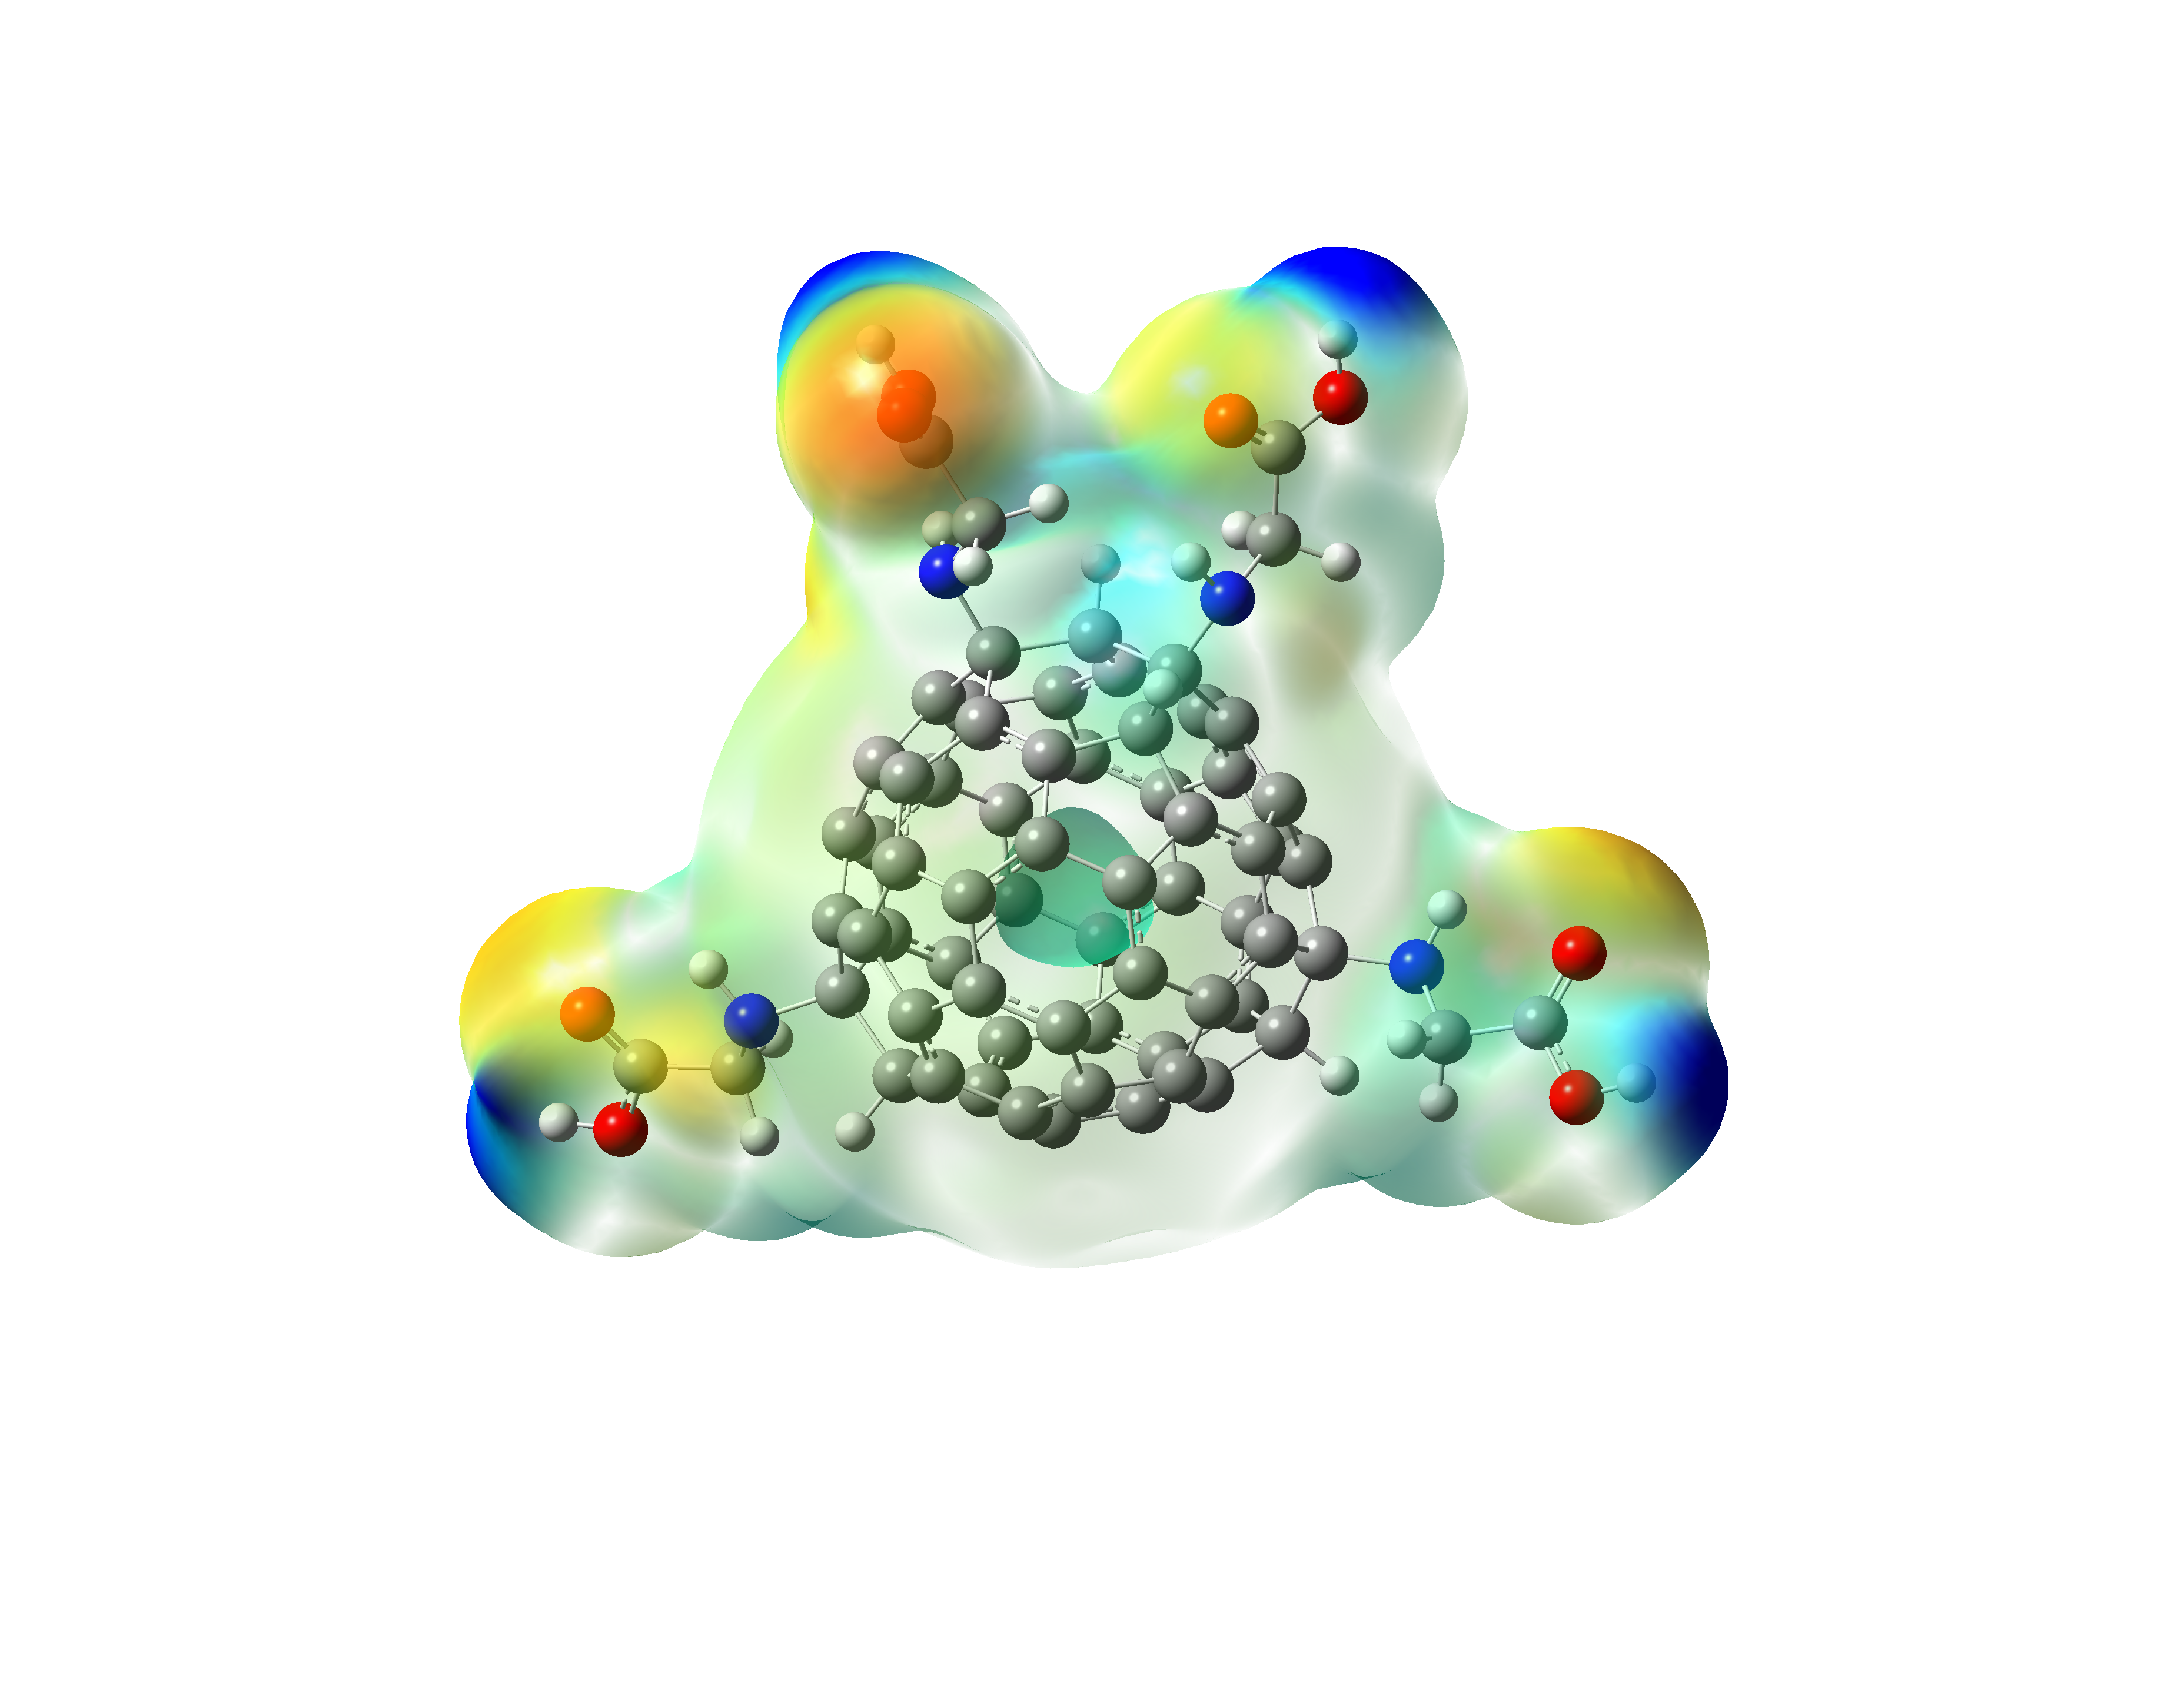
\includegraphics[width=0.6\textwidth,height=0.40\textwidth]{imagenes/Resultados/c60-4gli.png}
      \caption{\textbf{Mapa de potencial electrostático: regiones azules corresponden a zonas con carga positivas mientras las regiones rojas corresponden a zonas con carga negativa  C\textsubscript{60}(\textit{Gly})\textsubscript{4}}.}
\end{figure}
\end{frame}
%--------------------------------------------------------------------------------------------


%----------------------------------------------------------------------------------------------
\begin{frame}{Poder electroaceptor y electro donador del  C\textsubscript{60}(\textit{Gly})\textsubscript{4}}
\begin{equation}
AE = (E_{\text{neutro}} - E_{\text{anión}})       
\end{equation}
\begin{equation}
PI = (E_{\text{catión}} - E_{\text{neutro}})     
\end{equation}
\begin{columns}[t] % Alineación superior exacta para ambas columnas

    % === PRIMERA TABLA (COLUMNA IZQUIERDA) ===
    \begin{column}{0.48\textwidth}
        \begin{table}[H]
            \centering
            \small
            \caption{Descriptores globales de reactividad (PI, EA) para evaluar el poder electroacepctor y electrodonador del C\textsubscript{60}(\textit{Gly})\textsubscript{4}.}
            \label{tab:descriptores_reactividad1}
            \vspace{0.2cm}
            
            \begin{tabular}{ccc}
                \toprule
                \textbf{Sistema} & PI (eV) & AE (eV) \\
                \midrule
                 \textbf{C\textsubscript{60}}& 7.608 & 2.454
\\
                \textbf{C\textsubscript{60}(\textit{Gly})\textsubscript{4}} & 6.849
 & 1.779
\\
               
                \bottomrule
            \end{tabular}%
        \end{table}
    \end{column}

    % === SEGUNDA TABLA (COLUMNA DERECHA) ===
  

\end{columns}
\end{frame}

%------------------------------------------------------------------------------------------------


%---------------------------------------------------------------------------

\begin{frame}{Delimitación del espacio de búsqueda tridimensional}
\begin{columns}
\begin{column}{0.3\textwidth}
\vspace*{-1.5cm}

\begin{table}[H]
\centering
\caption{Parámetros geométricos de la rejilla de acoplamiento para el complejo C\textsubscript{60}(\textit{Gly})\textsubscript{4} -- NS2B/NS3.}
\label{tab:parametros_acoplamiento}
\resizebox{\linewidth}{!}{%
\begin{tabular}{lccc} % Usa 'l' para alinear los parámetros a la izquierda y 'c' para centrar los valores
\toprule
\textbf{Parametros geométricos} 
& \textbf{Eje x} &\textbf{Eje y} &\textbf{Eje z}\\
\midrule
Número de puntos & 60 & 66 & 68 \\
Coordenadas del centro & 48.485 & 51.847 & 57.983 \\
\bottomrule
\end{tabular}%
}
\end{table}

\end{column}


\begin{column}{0.7\textwidth}
\begin{figure}[h]
    \centering
    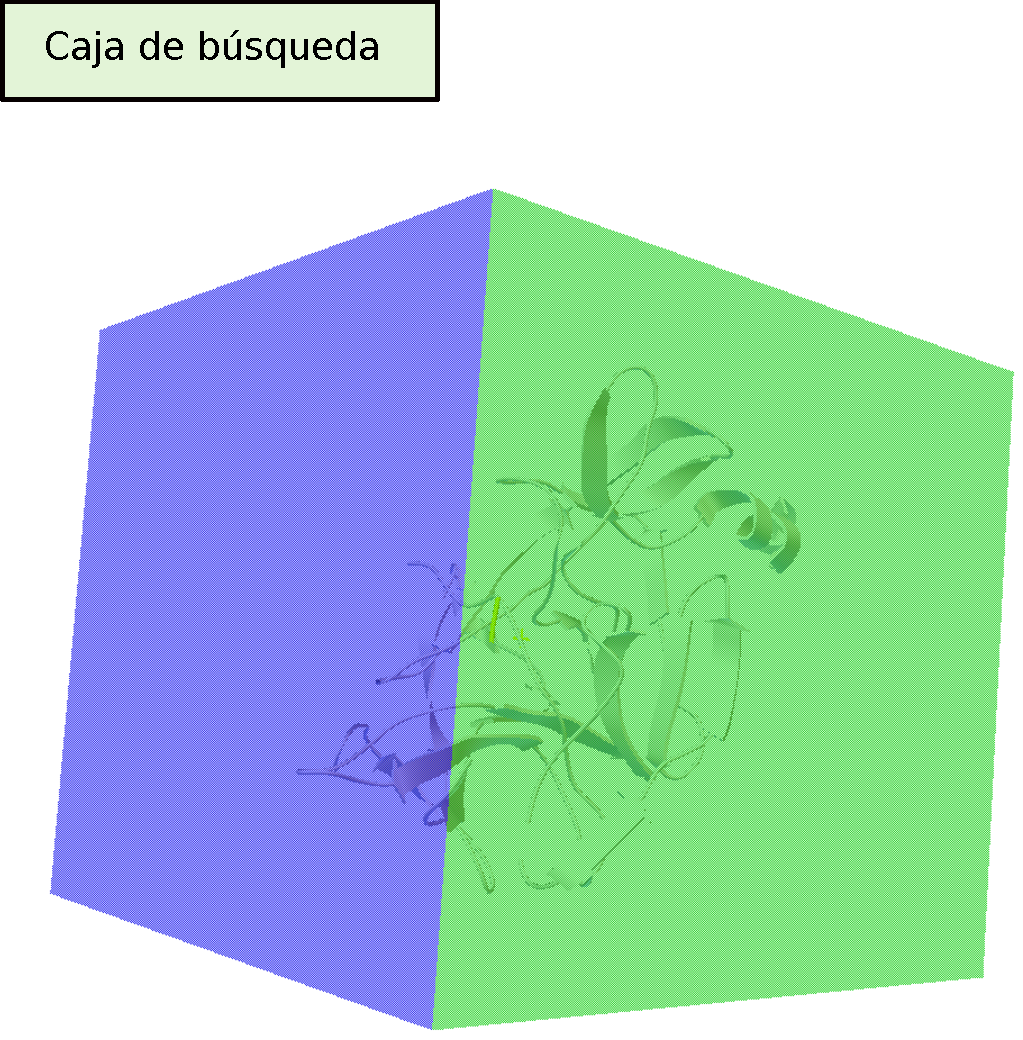
\includegraphics[width=0.7\textwidth,height=0.6\textwidth]{imagenes/Resultados/box-1.pdf}
      \caption{\textbf{Visualización de la rejilla para el acoplamiento de C\textsubscript{60}(\textit{Gly})\textsubscript{4}-NS2B-NS3.}}
\end{figure}

\end{column}
\end{columns}
\end{frame}




%---------------------------------------------------------------------------


%------------------
\begin{frame}{Análisis de clusters y distribución de energías de unión}
\begin{figure}[h]
\vspace*{-0.30cm}
    \centering
    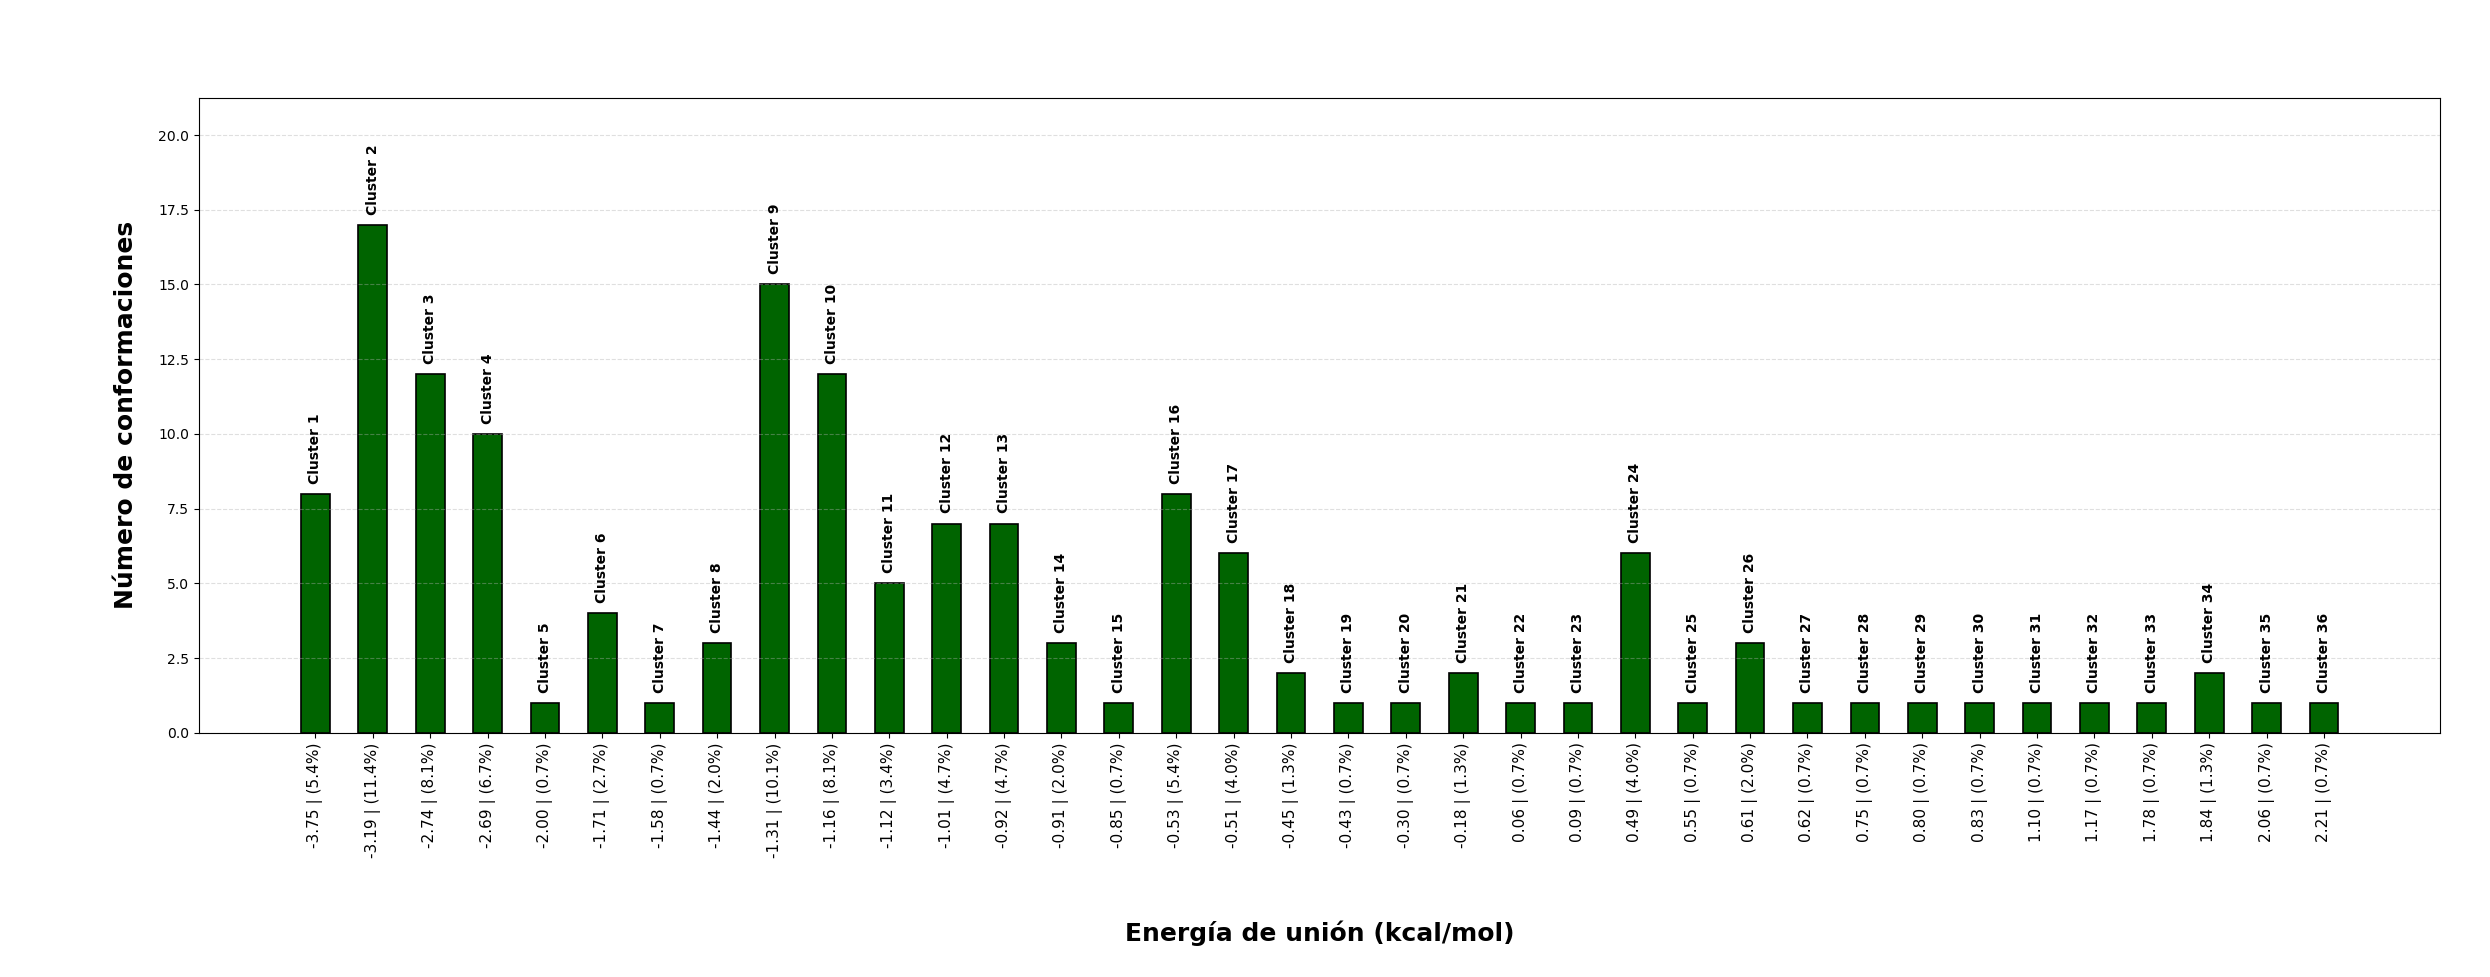
\includegraphics[width=0.9\textwidth,height=0.5\textwidth]{imagenes/Resultados/histograma-completo.png}
      \vspace*{-0.45cm}
      \caption{\textbf{ Histograma de agrupamiento conformacional de las poses del ligando C\textsubscript{60}(\textit{Gly})\textsubscript{4} en el sitio alostérico de la proteína 2FOM. El análisis se realizó empleando una tolerancia de 8 \AA.}}
\end{figure}

\end{frame}
%_____________-----------------------------------------------------------------

\begin{frame}{Acoplamiento del C\textsubscript{60}(\textit{Gly})\textsubscript{4} con la proteína NS2B-NS3}
\begin{columns}
\begin{column}{0.3\textwidth}
\vspace*{-1.5cm}

\begin{table}[H]
\centering
\caption{Parámetros energéticos y constantes de afinidad del complejo C\textsubscript{60}(\textit{Gly})\textsubscript{4} -- NS2B/NS3 para el cluster de mayor convergencia.}
\label{tab:parametros_acoplamiento}
\resizebox{\linewidth}{!}{%
\begin{tabular}{lc} % Usa 'l' para alinear los parámetros a la izquierda y 'c' para centrar los valores
\toprule
\textbf{Parámetros} & \textbf{Valor de la energía} \\
\midrule
Energía de Unión & -3.19 \\
Eficiencia del Ligando & -0.04 \\
Constante de Inhibición & 4.62 \\
Energía Intermolecular & -9.75 \\
VdW + P. Hidrógeno + Desolv. & -7.5 \\
Energía Electrostática & -2.25 \\
Energía Interna Total & -6.66 \\
Energía Torsional & 6.56 \\
Energía del Sistema Libre & Libre -6.66 \\
\bottomrule
\end{tabular}%
}
\end{table}

\tiny Residuos: Val72, Trp50, Arg54, Asp75, His51, Val155, Tyr161, Pro132.



\end{column}


\begin{column}{0.7\textwidth}
\begin{figure}[h]
    \centering
    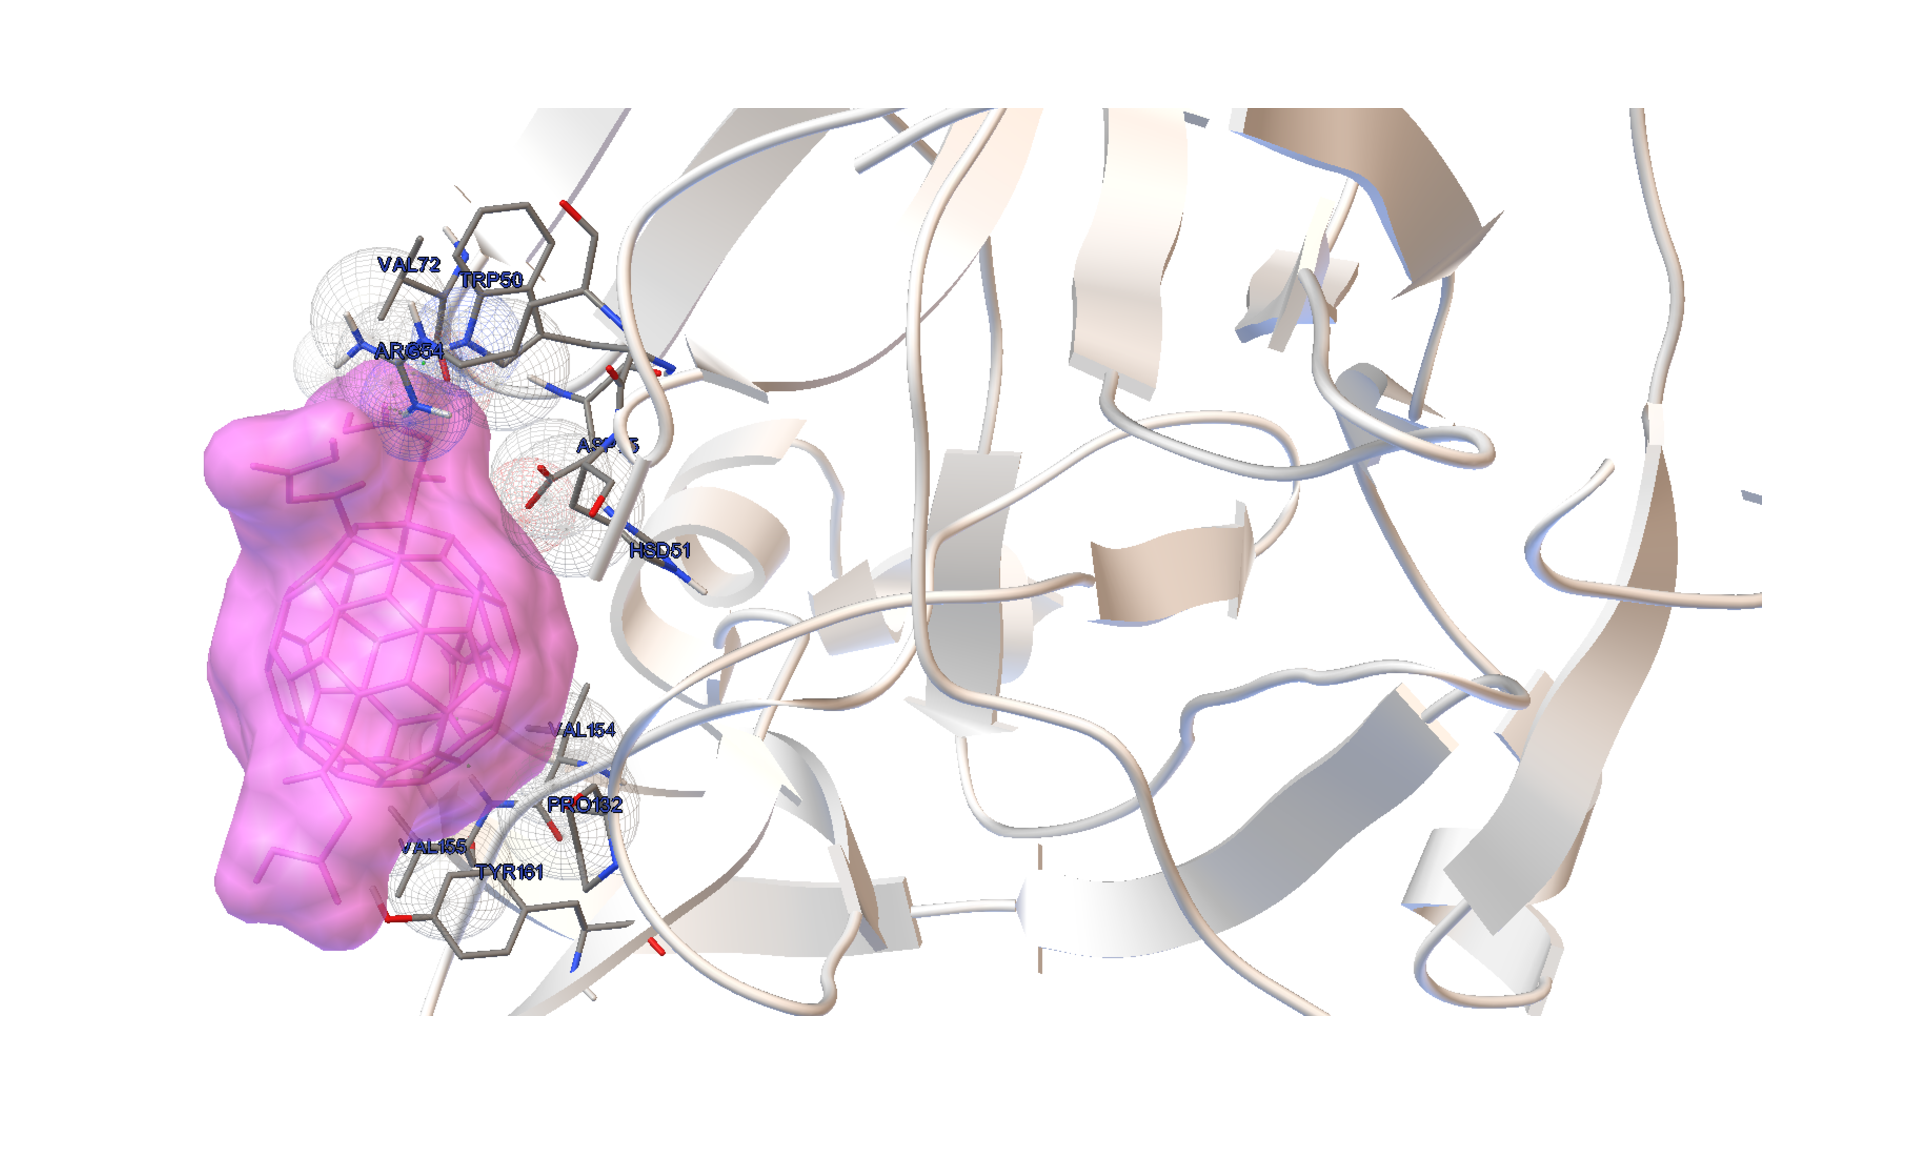
\includegraphics[width=1.0\textwidth,height=0.6\textwidth]{imagenes/Resultados/principal-acoplamiento.pdf}
      \caption{\textbf{Visualización de la pose de mayor afinidad del complejo C\textsubscript{60}(\textit{Gly})\textsubscript{4} NS2B-NS3.}}
\end{figure}

\end{column}
\end{columns}
\end{frame}
%---------------------------------------------------------------
\begin{frame}{Delimitación del espacio de búsqueda tridimensional}
\begin{columns}
\begin{column}{0.3\textwidth}
\vspace*{-1.5cm}

\begin{table}[H]
\centering
\caption{Parámetros geométricos de la rejilla de acoplamiento para el complejo C\textsubscript{60}(\textit{Gly})\textsubscript{4} -- NS2B/NS3.}
\label{tab:parametros_acoplamiento}
\resizebox{\linewidth}{!}{%
\begin{tabular}{lccc} % Usa 'l' para alinear los parámetros a la izquierda y 'c' para centrar los valores
\toprule
\textbf{Parametros geométricos} 
& \textbf{Eje x} &\textbf{Eje y} &\textbf{Eje z}\\
\midrule
Número de puntos & 118 & 118 & 126 \\
Coordenadas del centro & 47.785 & 45.840 & 54.561 \\
\bottomrule
\end{tabular}%
}
\end{table}

\end{column}


\begin{column}{0.7\textwidth}
\begin{figure}[h]
    \centering
    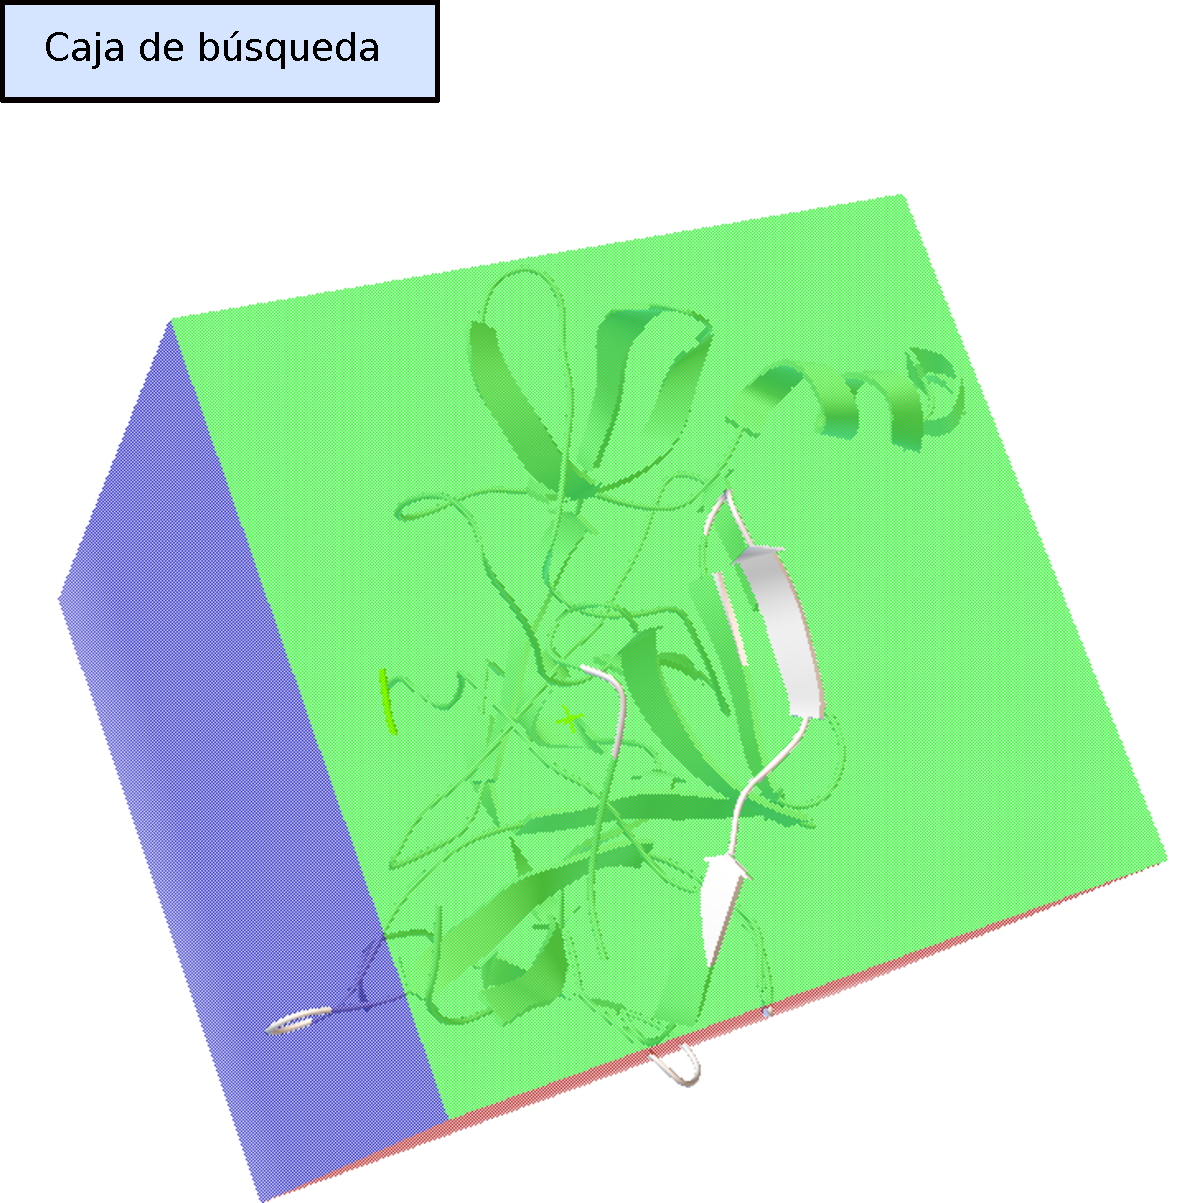
\includegraphics[width=0.7\textwidth,height=0.6\textwidth]{imagenes/Resultados/box-2.pdf}
      \caption{\textbf{Visualización de la rejilla para el acoplamiento de C\textsubscript{60}(\textit{Gly})\textsubscript{4}-NS2B-NS3.}}
\end{figure}

\end{column}
\end{columns}
\end{frame}

%--------------------------------------------------------------------------------


\begin{frame}{Análisis de clusters y distribución de energías de unión}
\begin{figure}[h]
\vspace*{-0.2cm}
    \centering
    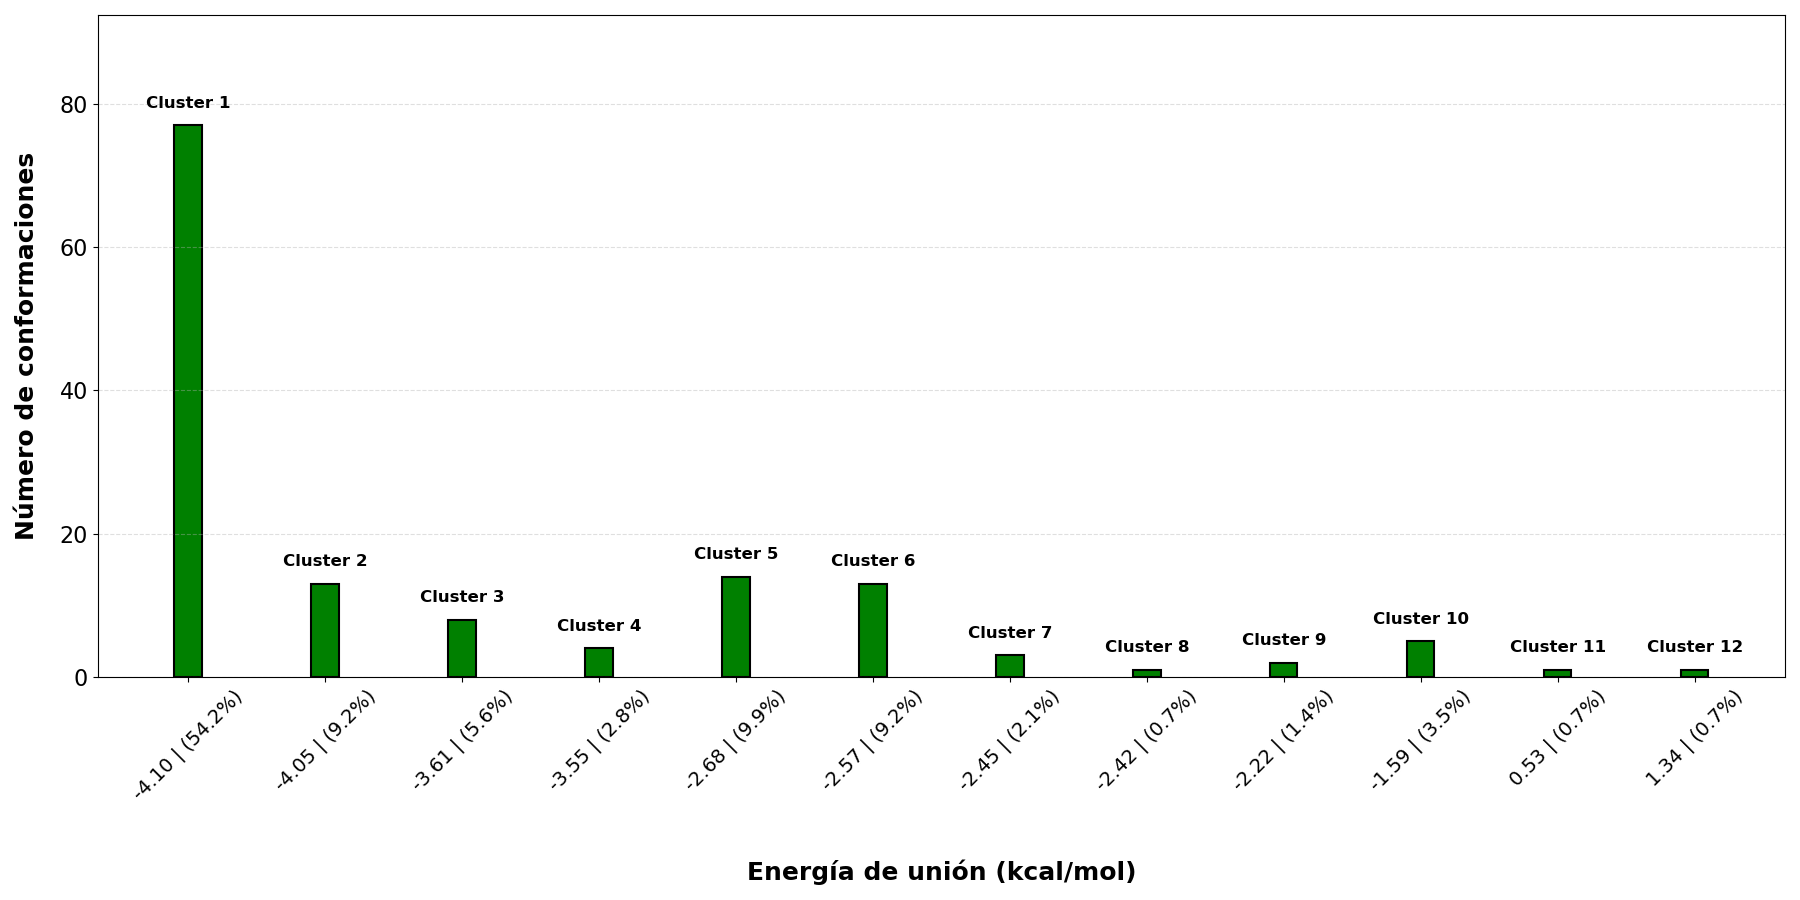
\includegraphics[width=0.8\textwidth,height=0.45\textwidth]{imagenes/Resultados/histograma-1.png}
    
      \caption{\textbf{ Histograma de agrupamiento conformacional de las poses del ligando C\textsubscript{60}(\textit{Gly})\textsubscript{4} en el sitio alostérico de la proteína 2FOM. El análisis se realizó empleando una tolerancia de 8 \AA. }}
\end{figure}

\end{frame}

%________------------------------------------------------------------------------
\begin{frame}{Acoplamiento del C\textsubscript{60}(\textit{Gly})\textsubscript{4} en el Sitio Alostérico de NS2B-NS3}
\begin{columns}
\begin{column}{0.3\textwidth}
\vspace*{-1.5cm}
\begin{table}[H]
\centering
\caption{Parámetros energéticos y constantes de afinidad del complejo C\textsubscript{60}(\textit{Gly})\textsubscript{4} -- NS2B/NS3 para el cluster de mayor convergencia.}
\label{tab:parametros_acoplamiento_cluster}
\resizebox{\linewidth}{!}{%
\begin{tabular}{lc}
\toprule
\textbf{Parámetros} & \textbf{Valor de la energía} \\
\midrule
Energía de Unión & -4.1 \\
Eficiencia del Ligando & -0.05 \\
Constante de Inhibición & 985.12 \\
Energía Intermolecular & -10.96 \\
VdW + P. Hidrógeno + Desolv. & -8.07 \\
Energía Electrostática & -2.89 \\
Energía Interna Total & -6.02 \\
Energía Torsional & 6.86 \\
Energía del Sistema Libre & Libre -6.02 \\
\bottomrule
\end{tabular}%
}
\end{table}
\tiny Residuos: Lys143, Glu63, Lys142, Trp61, Arg60.
\end{column}


\begin{column}{0.7\textwidth}
\begin{figure}[h]
    \centering
    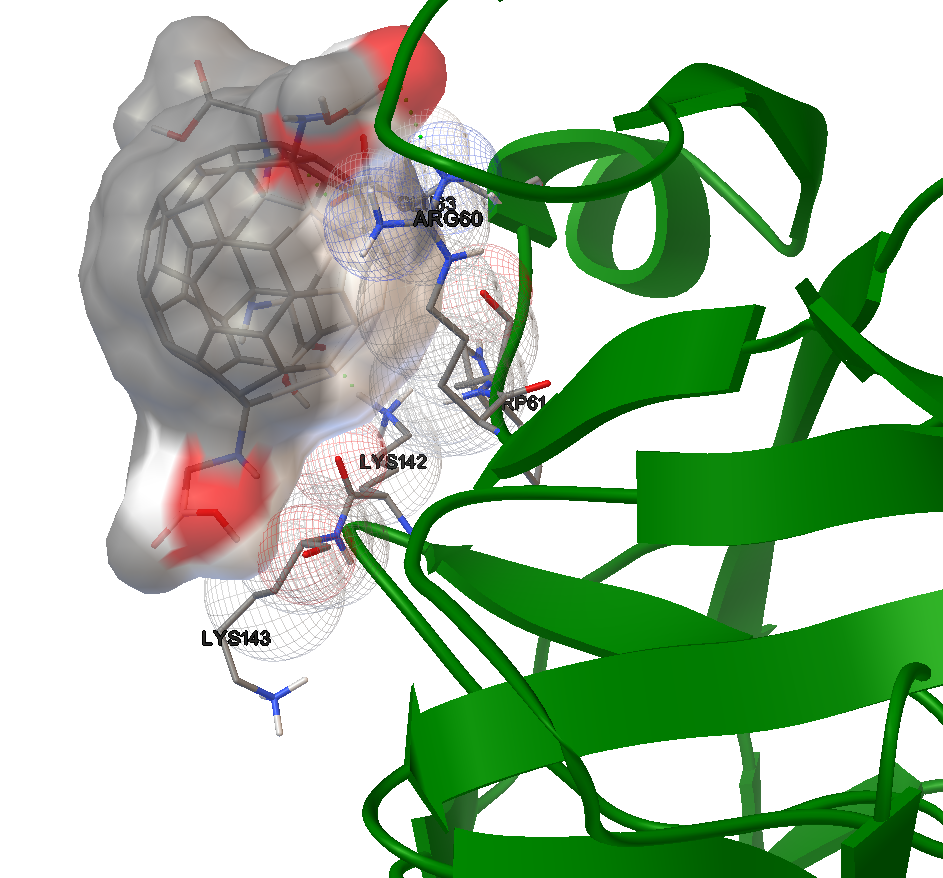
\includegraphics[width=0.9\textwidth,height=0.5\textwidth]{imagenes/Resultados/primera-pose.png}
      \caption{\textbf{Visualización de la pose de mayor afinidad del complejo C\textsubscript{60}(\textit{Gly})\textsubscript{4} NS2B-NS3.}}
\end{figure}

\end{column}
\end{columns}
\end{frame}

%-----------------------------------------------------------------
\begin{frame}{Acoplamiento del C\textsubscript{60}(\textit{Gly})\textsubscript{4} en el Sitio Alostérico de NS2B-NS3}
\begin{columns}
\begin{column}{0.33\textwidth}
\begin{figure}[h]
    \centering
    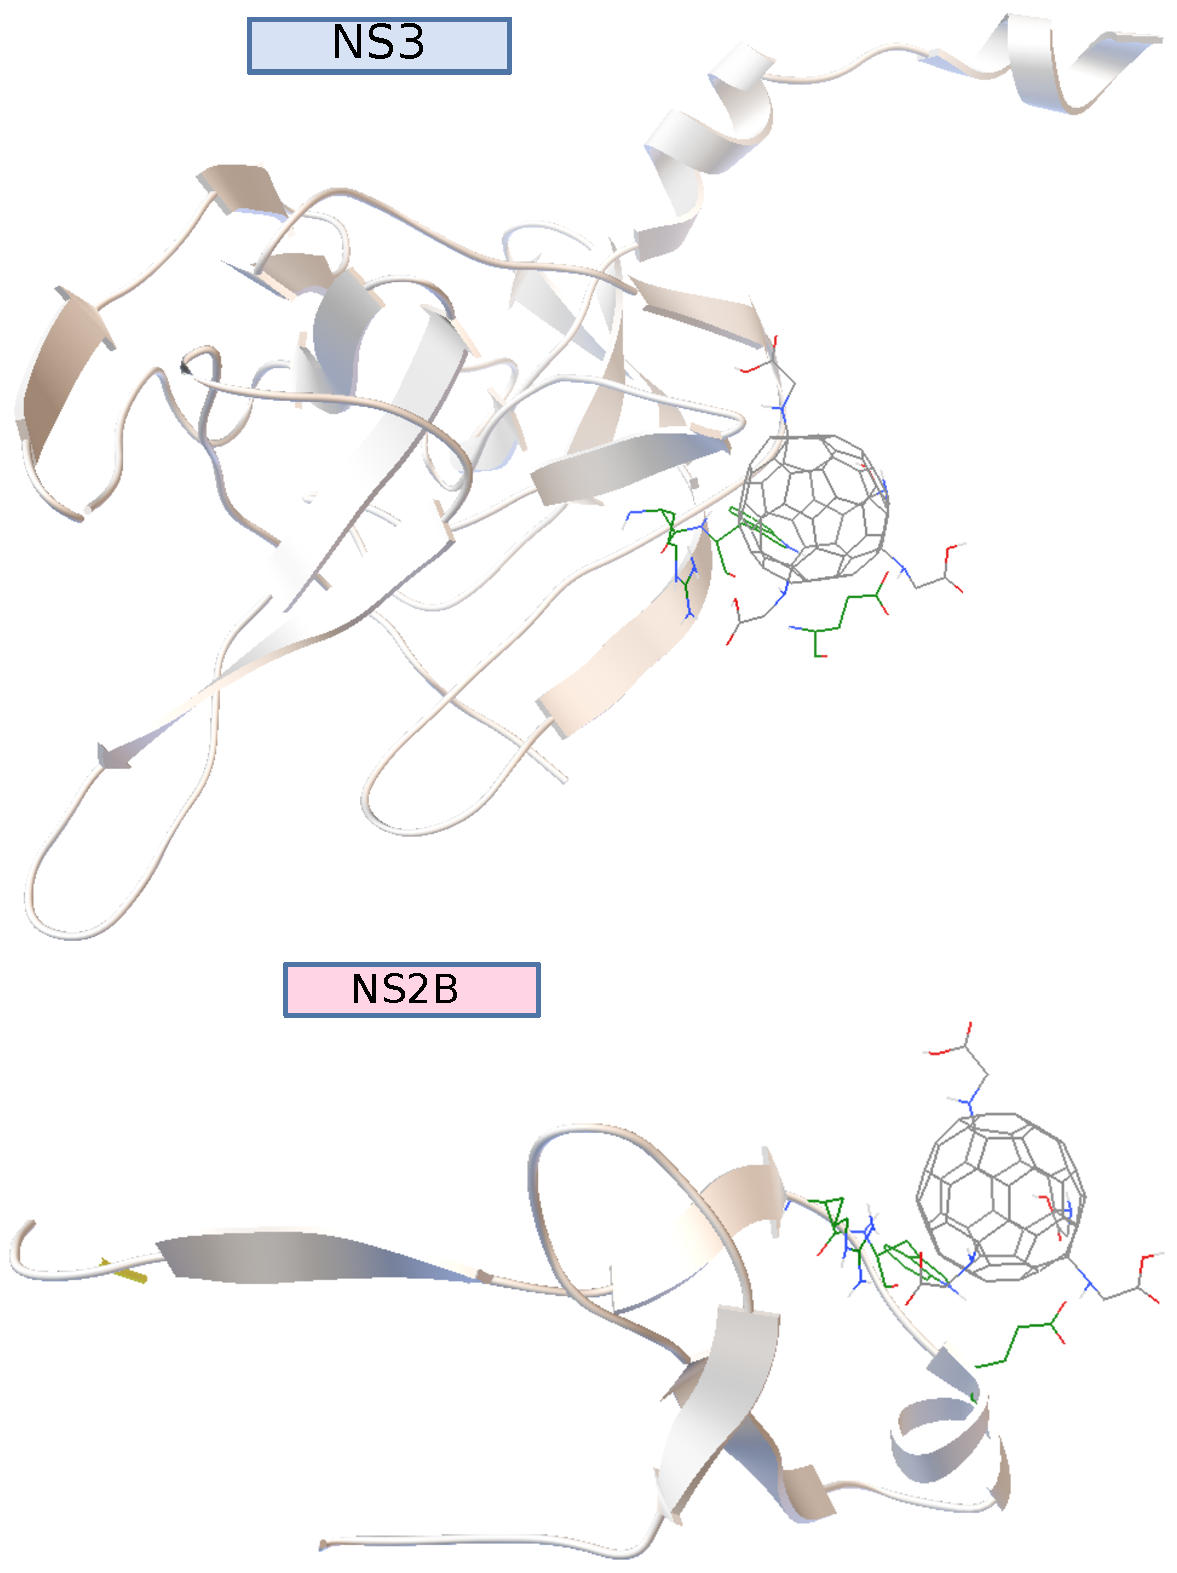
\includegraphics[width=0.8\textwidth,height=0.9\textwidth]{imagenes/Resultados/sitio-1.pdf}
      \caption{\textbf{ Representación del acoplamiento de NS2B-NS3 con el ligando C\textsubscript{60}(\textit{Gly})\textsubscript{4}. }}
\end{figure}
\end{column}
\begin{column}{0.33\textwidth}
\begin{figure}[h]
    \centering
    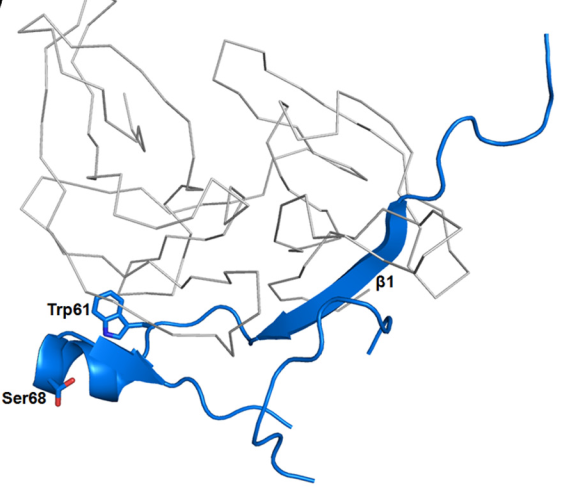
\includegraphics[width=0.9\textwidth,height=0.8\textwidth]{imagenes/Resultados/sitio-articulo.png}
      \caption{\textbf{ Conformación estructural del cofactor NS2B (azul) acoplado a la proteasa NS3 (gris) en DENV2, resaltando la ubicación de los residuos \textbf{Trp61} y \textbf{Glu63}. }}
\end{figure}

\end{column}

\begin{column}{0.33\textwidth}
\justifying  \\
La región entre \textbf{Trp61} y \textbf{Glu63} dirige la transición estructural. Para activar el complejo, el cofactor NS2B pasa de un estado inactivo extendido a acoplarse estrechamente sobre NS3 \cite{yao2019discovery, chandramouli2010serotype}.
\vspace*{1cm}

\scriptsize{\cite{yao2019discovery}} Yao, Y. et al.,\emph{Journal of the American Chemical Society}, 2019. \\
\scriptsize{\cite{chandramouli2010serotype}} Chandramouli, S. et al.,\emph{Journal of Virology}, 2010.
\end{column}
\end{columns}
\end{frame}
%-----------------------------------------------------------------------------------------

\begin{frame}{Acoplamiento del C\textsubscript{60}(\textit{Gly})\textsubscript{4} en el Sitio Alostérico de NS2B-NS3}
\begin{columns}
\begin{column}{0.3\textwidth}
\vspace*{-1.5cm}
\begin{table}[H]
\centering
\caption{Parámetros energéticos y constantes de afinidad del complejo C\textsubscript{60}(\textit{Gly})\textsubscript{4} -- NS2B/NS3 para el cluster con Ile67.}
\label{tab:parametros_acoplamiento_ile67}
\resizebox{\linewidth}{!}{%
\begin{tabular}{lc}
\toprule
\textbf{Parámetros} & \textbf{Valor de la energía} \\
\midrule
Energía de Unión & 0.7 \\
Eficiencia del Ligando & 0.01 \\
Constante de Inhibición & 985.12 \\
Energía Intermolecular & -6.16 \\
VdW + P. Hidrógeno + Desolv. & -4.17 \\
Energía Electrostática & -1.99 \\
Energía Interna Total & -9.62 \\
Energía Torsional & 6.86 \\
Energía del Sistema Libre & Libre -9.62 \\
\bottomrule
\end{tabular}%
}
\end{table}
\end{column}


\begin{column}{0.7\textwidth}
\begin{figure}[h]
    \centering
    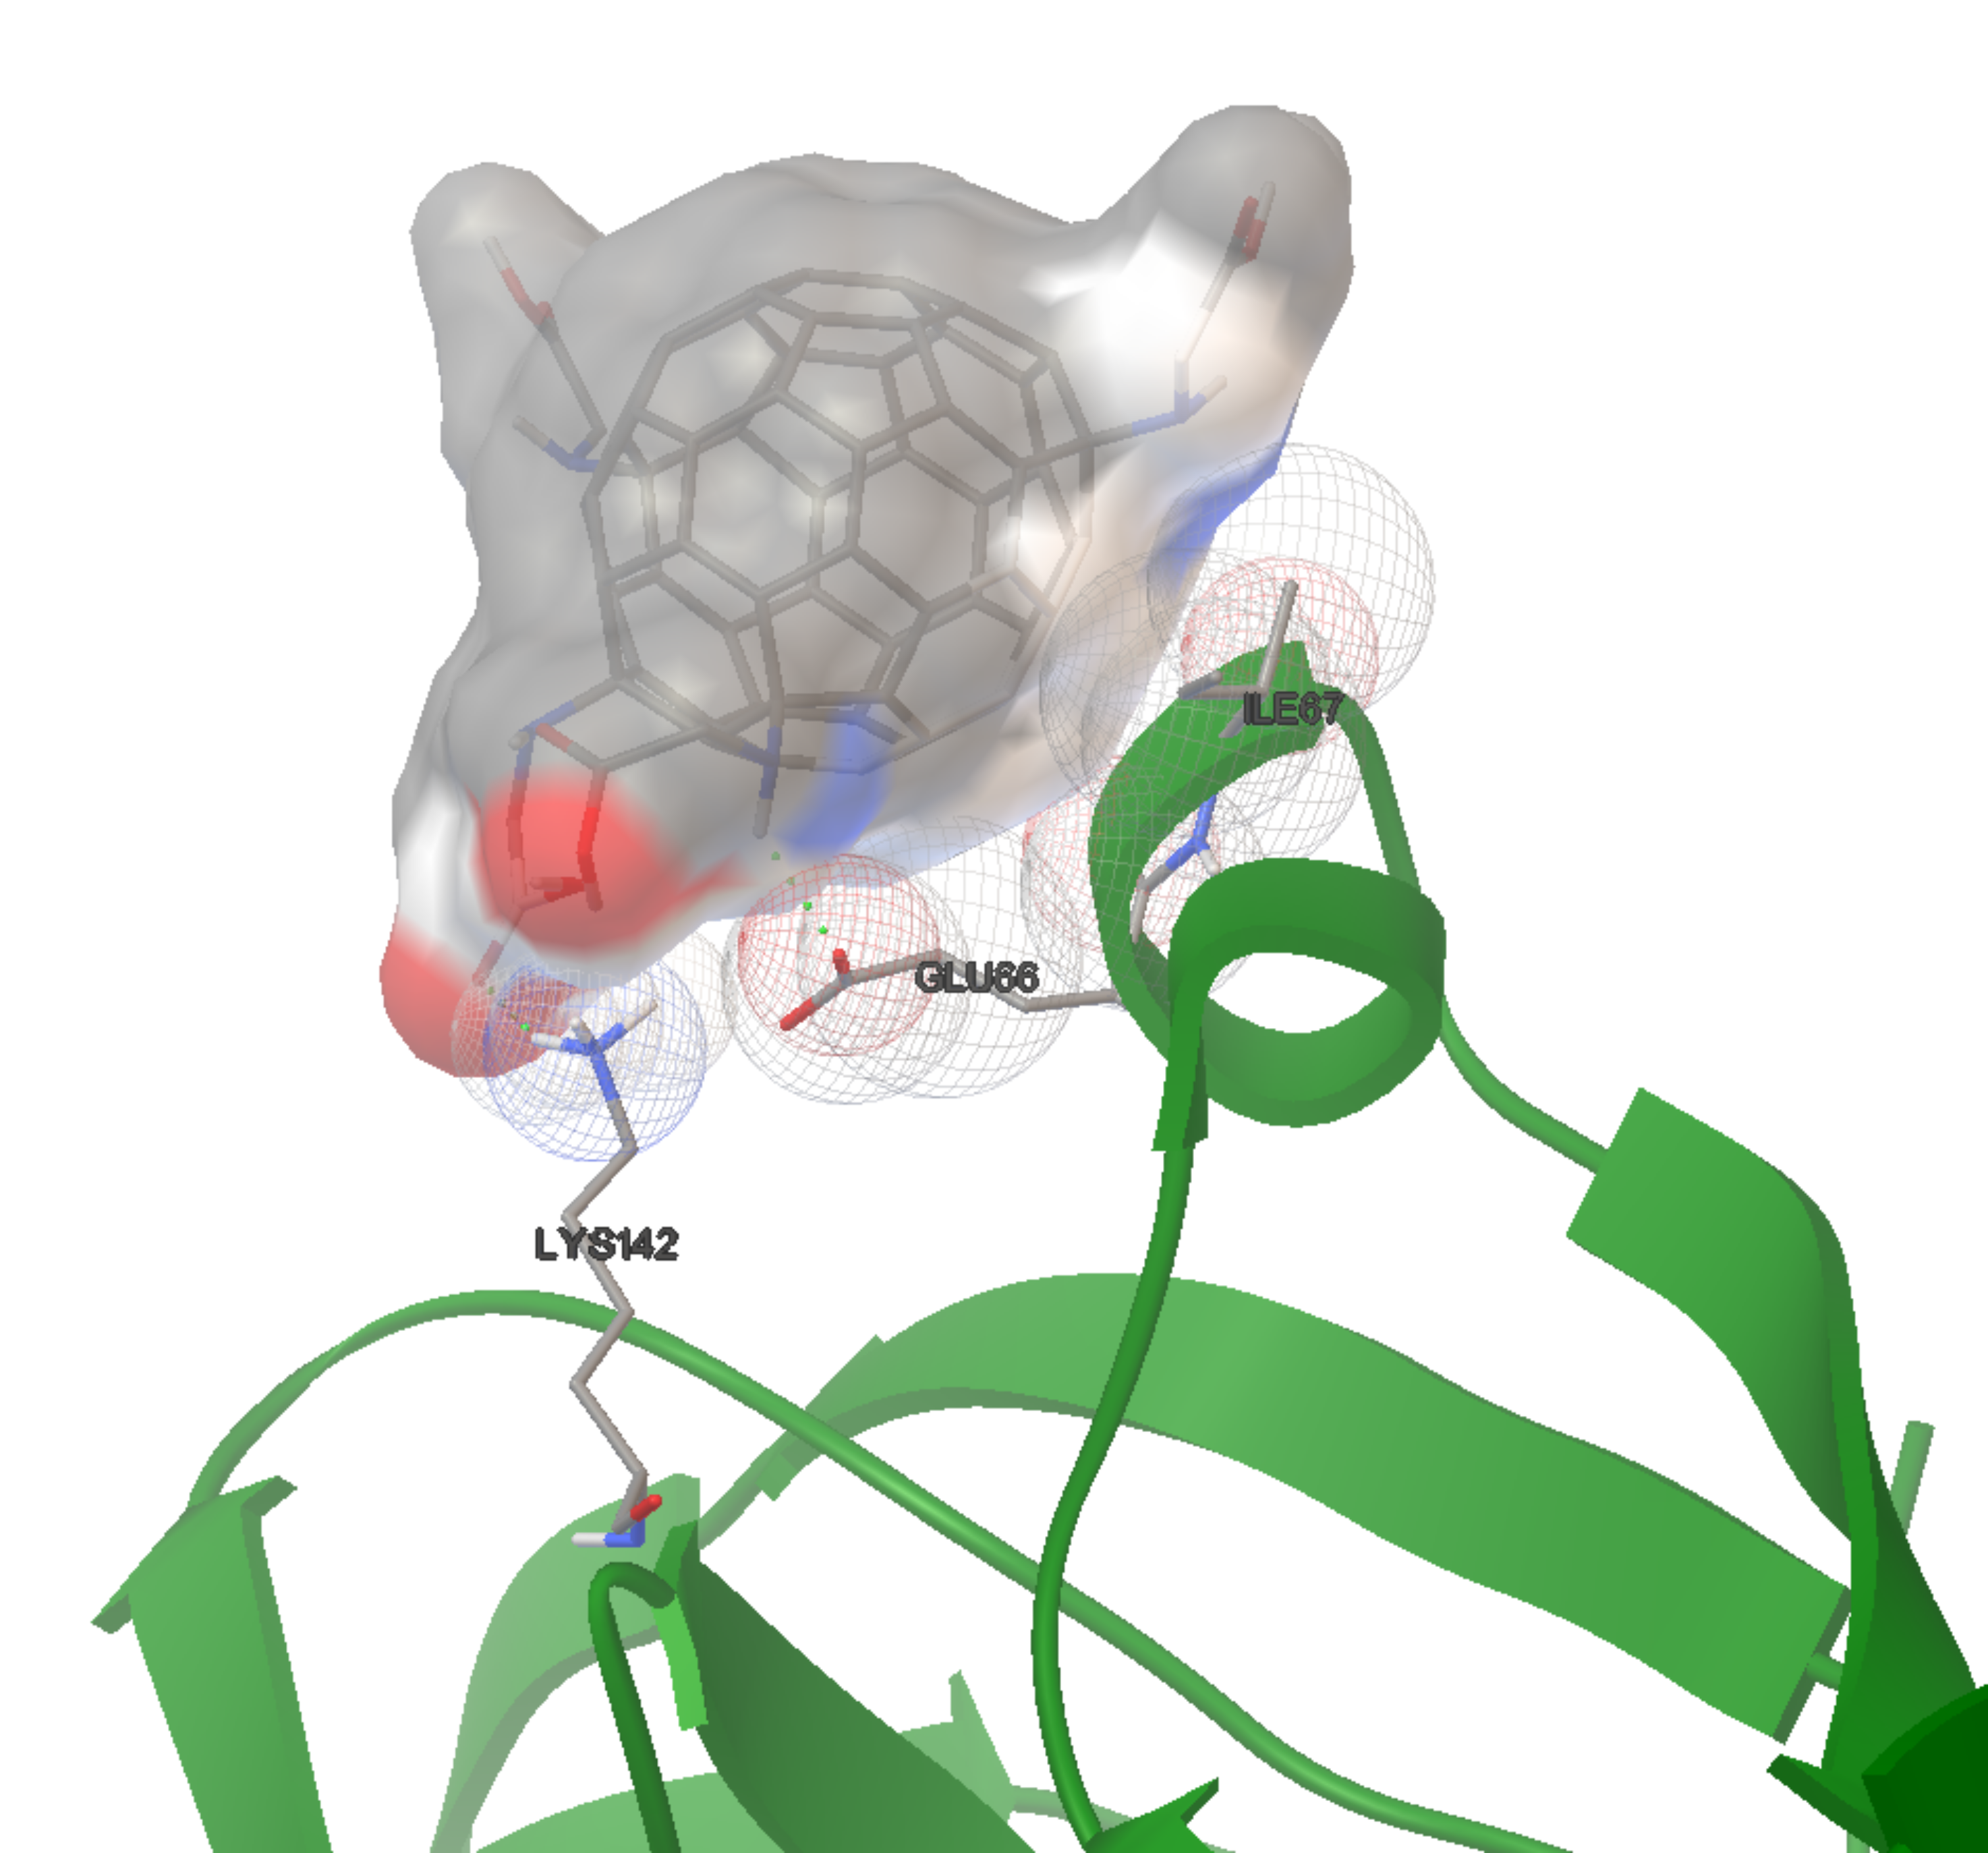
\includegraphics[width=0.9\textwidth,height=0.5\textwidth]{imagenes/Resultados/ileu67.png}
      \caption{\textbf{ Representación del acoplamiento de NS2B-NS3 con el ligando C\textsubscript{60}(\textit{Gly})\textsubscript{4} y los residuos correspondientes. }}
\end{figure}

\end{column}
\end{columns}
\end{frame}

%------------------------------------------------------------------------------------------------------------------------



%-------------------------------------------------------------------------------------


\section{Conclusiones}
\begin{frame}[allowframebreaks]{Conclusiones}
\begin{itemize}
\justifying
\item Los cálculos de estructura electrónica confirmaron que la funcionalización del complejo C\textsubscript{60}(\textit{Gly})\textsubscript{4} modifica favorablemente sus propiedades físico-químicas, confiriéndole las características necesarias para interactuar en las regiones de interés, y manteniendo a su vez la capacidad del fullereno como aceptor de electrones.

\item El análisis de acoplamiento molecular demostró que el aducto  es capaz de interactuar con el complejo proteico NS2B-NS3 del virus del Dengue (DENV2). La evaluación mediante un acoplamiento dirigido arrojó una energía de unión favorable, identificándose un clúster con más del 50\% de sus poses óptimas. Estos resultados brindan información valiosa sobre las interacciones específicas en los sitios de interés, demostrando que el sistema puede unirse de manera estable en las regiones reportadas.

\end{itemize}
\end{frame}

\section{Perspectivas}
\begin{frame}[allowframebreaks]{Perspectivas}
En trabajos futuros se pretende:
\begin{itemize}
\justifying
 \item Nuevo acoplamiento dirigido para la proteína en conformacion abierta-inactiva.
 \item Acoplamiento molecular con la proteína en conformación cerrada-activa.
    \item Dinámica del complejo proteína-ligando. 
   
\end{itemize}

\end{frame}

\section{Cronograma}
\begin{frame}{Cronograma de actividades}
\vspace*{-0.3cm}
\begin{figure}
    \centering
    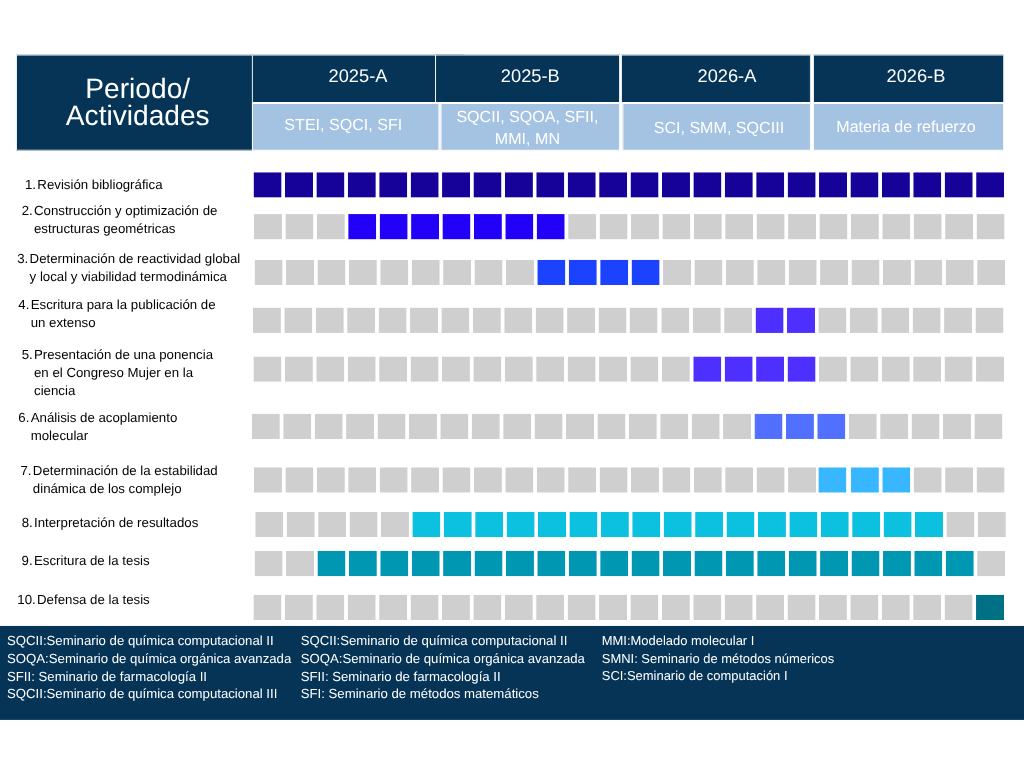
\includegraphics[width=0.9\textwidth,height=0.5\textwidth]{imagenes/metodologia/cronograma.png}
    \vspace*{-0.5cm}
    \textbf{\caption{Cronograma de actividades}
    \label{met:1} }%Esto genera un numero a mi etiqueta
\end{figure} 
\end{frame}



% Referencias ------------------------------------------------------------
\setbeamertemplate{footline}[empty]
\section{Referencias}
\scriptsize 
\begin{frame}[allowframebreaks] 
        \frametitle{Referencias}
        \bibliographystyle{ieeetr}
        \bibliography{ref.bib}
\end{frame}
\backmatter
\begin{frame}{Componentes de la proteína NS2B-NS3}

\begin{columns}
\justifying
\begin{column}{0.6\textwidth}
\begin{figure}
    \centering
    \includegraphics[width=0.6\textwidth, height=0.6\textwidth]{~/Tesis-Template-2/imagenes/Intro/bolsillos.png} 
  \textbf{ \caption{\justifying Representación que muestra solo las cadenas laterales y los esqueletos de los aminoácidos relevantes de NS2B-NS3. La superficie rosa claro es de NS3 y la violeta de NS2B; S1 está resaltada en naranja claro, S2 en verde, S3 en amarillo claro, S4 en aguamarina y S1’ en rosa oscuro.\cite{lescar2008towards, li2020insights}.}}
    \label{dete} %Esto genera un numero a mi etiqueta
\end{figure} 
\end{column}
\begin{column}{0.4\textwidth}
\vspace*{-2.0cm}
%-----------------------------------------------------------------------




%DEBO QUITAR ESTA PERO SI QUIERO LA PUEDO VOLVER A PONER

\begin{table}[h]
\caption{Componentes críticos del complejo NS2B-NS3.}
\centering
\tiny

% Hemos quitado el resizebox para que la letra no se haga pequeña
\begin{tabular}{|c|c|p{2.0cm}|} % Ajusta el 5.5cm si necesitas más o menos ancho
    \hline
    \textbf{Componente} & \textbf{Residuo} & \textbf{Función / Característica} \\ \hline
    
    \textbf{NS2B} & 49-95 & Porción hidrofílica esencial; evita la agregación de NS3 y activa la catálisis. \\ \hline
    
    \textbf{Bolsillo S1} & Asp129 & Carga negativa: Atrae residuos positivos (Arg/Lys) por electrostática. \\ \hline
    
    \textbf{Bolsillo S2} & Gly83 & Estabiliza al residuo P2 del sustrato mediante enlaces de hidrógeno. \\ \hline
    
    \textbf{NS3} & \begin{tabular}[c]{@{}c@{}}His51, Asp75,\\ Ser135\end{tabular} & \textbf{Tríada Catalítica:} Sitio central donde ocurre la reacción química de corte. \\ \hline
\end{tabular}
\end{table}

\scriptsize{\cite{lescar2008towards} Lescar, J. et al., \emph{Antiviral Res}, 2008.}\\
\scriptsize{\cite{li2020insights} Li, Q. \& Kang, C., Int. J. Mol. Sci. 2020.}
\end{column}
\end{columns}
\end{frame}

\begin{frame}{Ciclo de replicación del DENV}
\justifying
\begin{figure}
    \centering
    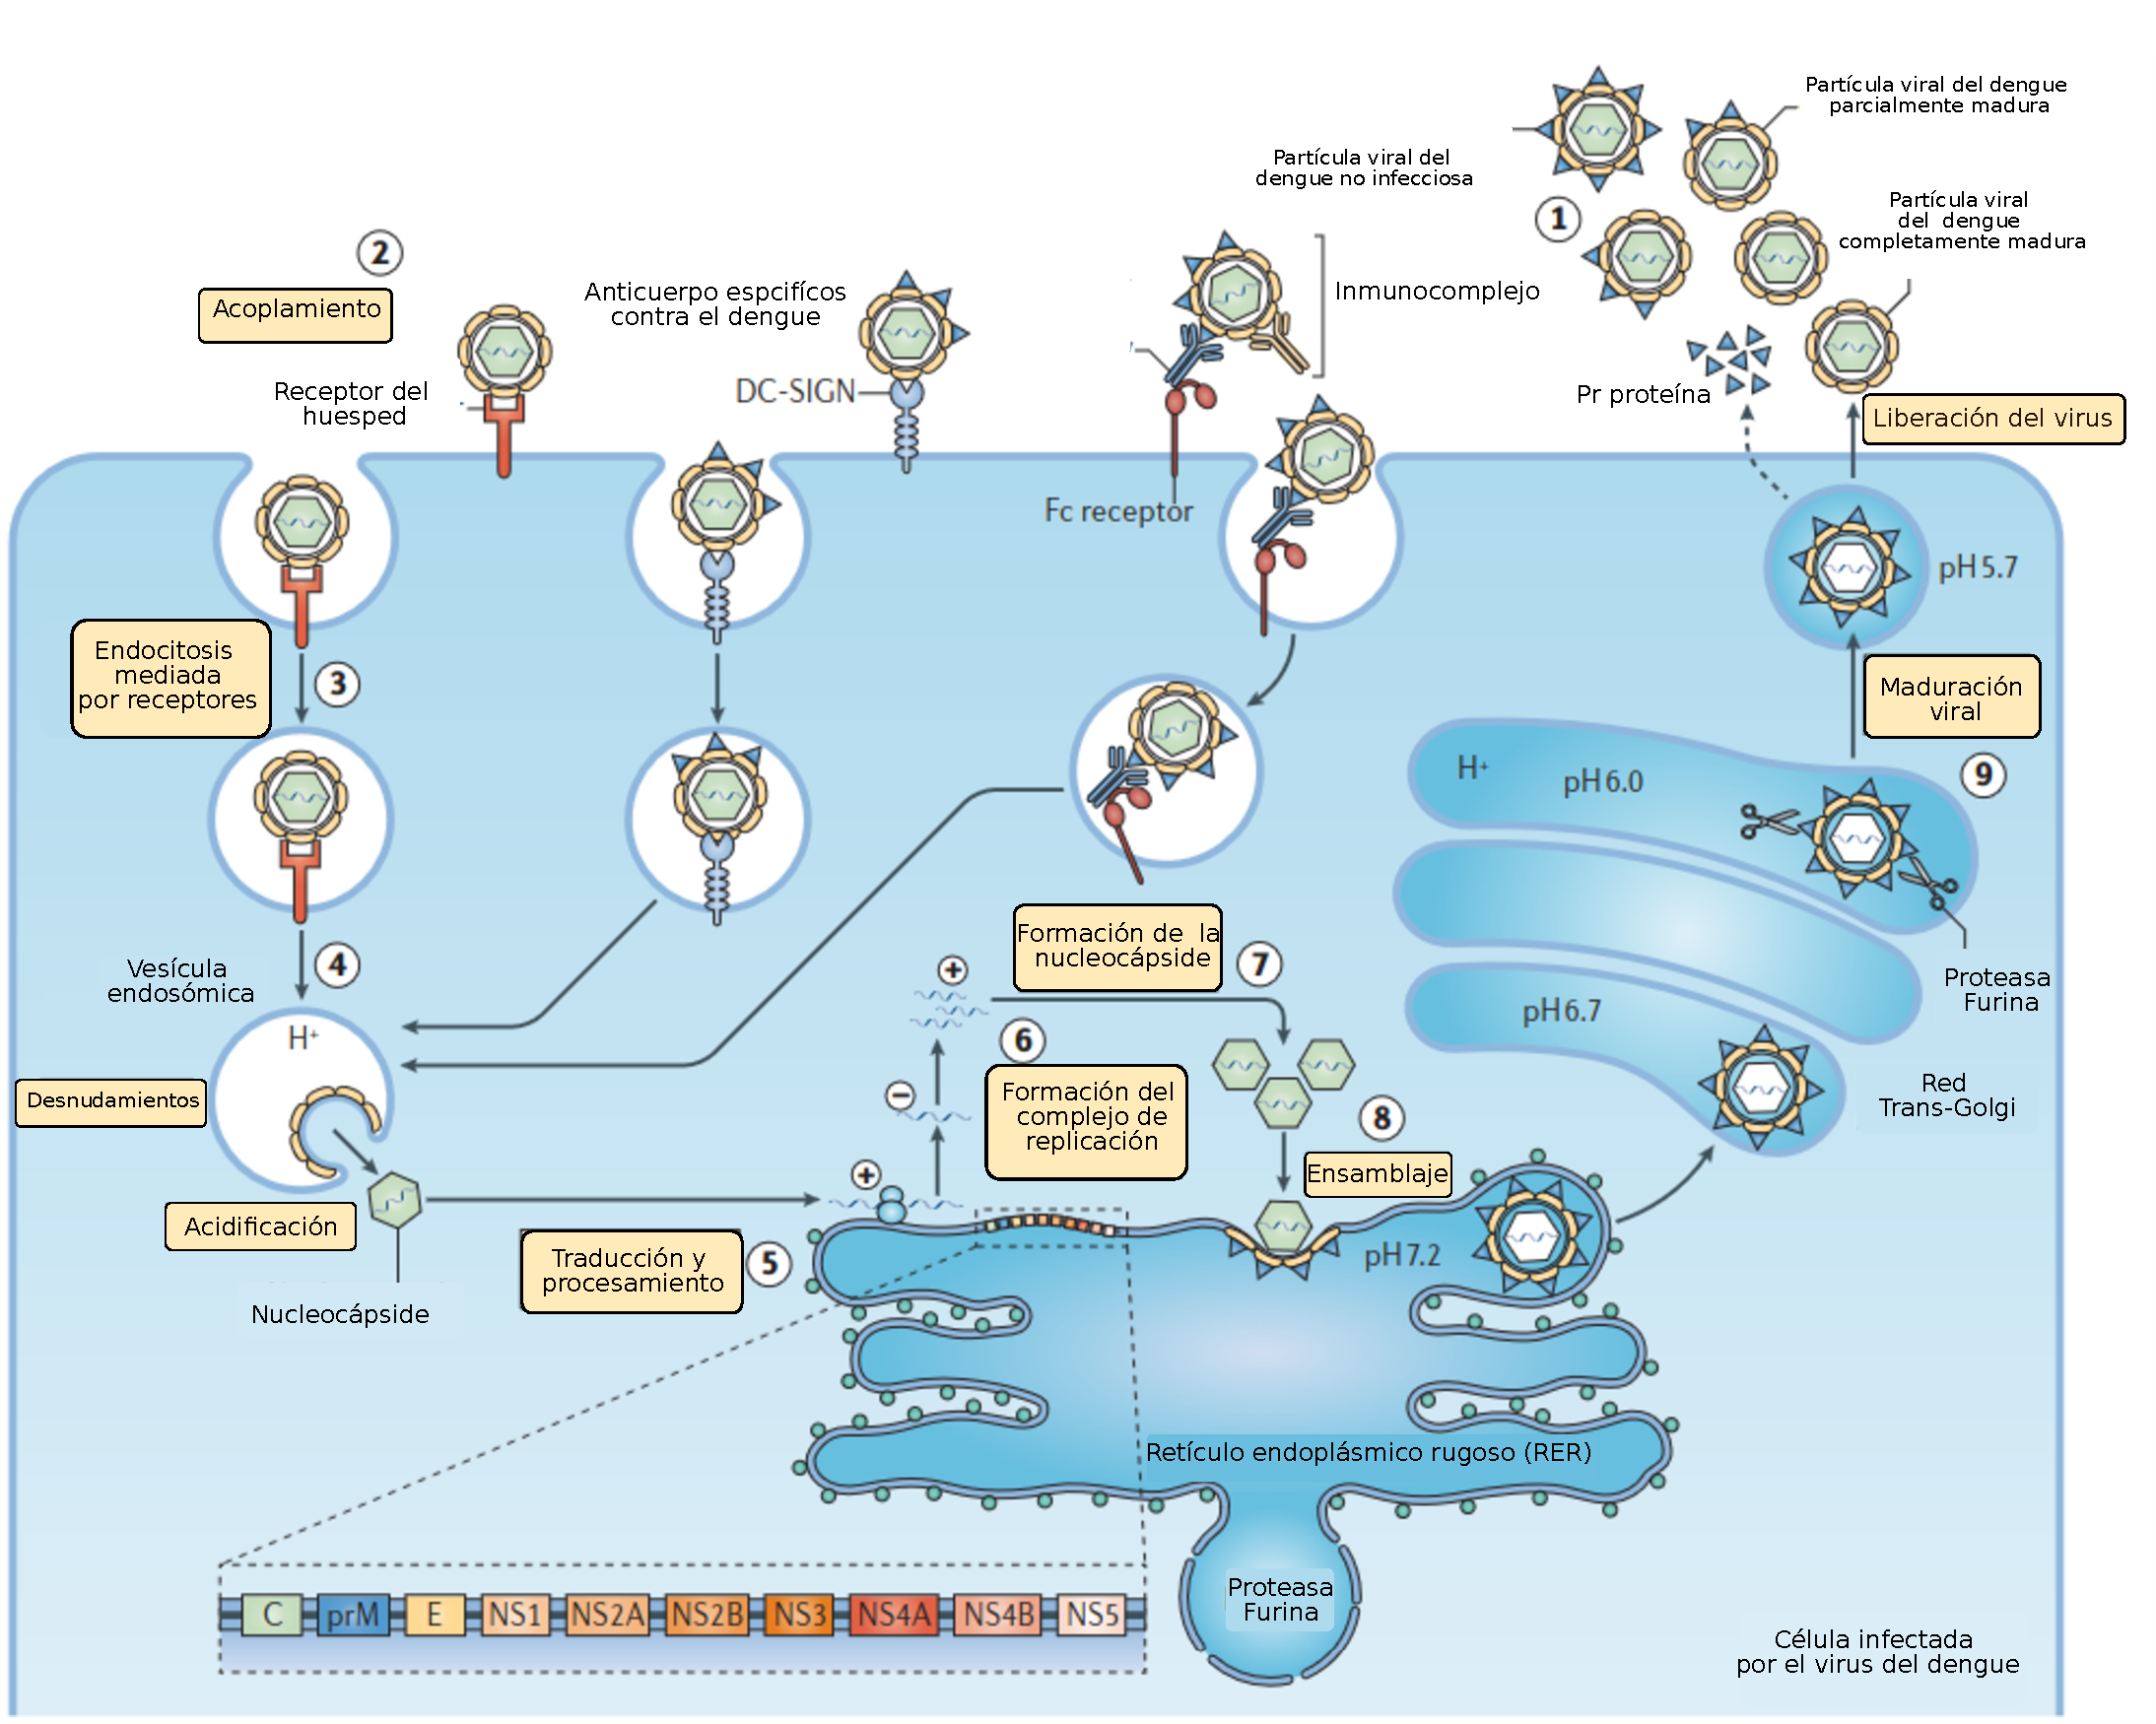
\includegraphics[width=0.75\textwidth, height=0.48\textwidth]{imagenes/Intro/ciclo-1.pdf} 
\vspace*{-0.25cm
    \caption{\justifying \textbf{Proceso de replicación del virus del dengue} \cite{screaton2015new}.}}
    \label{solarcell} %Esto genera un numero a mi etiqueta
\end{figure} 


\end{frame}





\begin{frame}{Funcionales de Intercambio y Correlación}
\small
\renewcommand{\arraystretch}{1.0} % Menor espacio entre filas
\begin{center}
\begin{tabular}{
    m{1.2cm}  % Funcional
   % m{1.9cm}  % Tipo
    %m{2.6cm}  % Intercambio
    %m{2.2cm}  % Correlación
    m{10cm}  % Características clave
}
\toprule
Funcional  & Características clave \\
\midrule
B3LYP & Muy usado en química molecular, buena precisión general \\
BP86 & Ligero, sin intercambio exacto, rápido \\
HSE06 & Ideal para materiales, reduce error de largo alcance \\
M06-2X & Buenos aproximando energías de activación \\
PBEPBE & Sin parámetros empíricos, base para otros funcionales \\
PBE1PBE (PBE0) & Balance entre precisión y costo computacional \\
\bottomrule
\end{tabular}
\end{center}
\textbf{\textcolor{red}{Conjuntos base}: 6-31G, 6-311G, 6-31G(d,p), 6-311G(d,p), 6-31++G(d,p) y 6-311++G(d,p).}
\end{frame}

\begin{frame}{\textit{Density Functional Theory}}
La teoría del funcional de la densidad (DFT) es una forma de aproximar la solución de la ecuación de Schrödinger para muchos electrones \cite{kohn1965self}.
\begin{gather}
       \rho(\Vec{r})=\sum_{1}^{N}\sum_{s}|\psi_{i}(\Vec{r},s)|^{2} \\
       V_{ef}=V_{ext}(\Vec{r})+\int \frac{\rho(\Vec{r})}{|\Vec{r}-\Vec{r'}|}+V_{xc} \\
       \left[ \frac{1}{2}\nabla^{2} +V_{ef}(a\Vec{r}) \right] \psi_{i}=\epsilon_{i}\psi_{i} \quad \quad (i=1,2, ... n) \\
       \begin{array}{c}
          E[ \rho(\Vec{r})]=\sum_{1}^{N}\sum_{s} \int \psi^{*}(\Vec{r}) \left( -\frac{1}{2}\nabla^{2} \right) \psi_{i}(\Vec{r})d^{3}\Vec{r} \quad + \quad \\ \frac{1}{2} \int \int  \frac{\rho(\Vec{r_{1}})\rho(\Vec{r_{2}})}{|\Vec{r_{1}}-\Vec{r'_{2}}|}d^{3}\Vec{r_{1}} d^{3}\Vec{r_{2}} + \int V(\Vec{r})\rho(a\Vec{r})d^{3}\Vec{r} + E_{xc}
       \end{array}
\end{gather}
\end{frame}
\begin{frame}{Funcionales de Intercambio y Correlación}

\begin{columns}
\begin{column}{0.5\textwidth}
\justifying
Un funcional \textcolor{red}{$F[\rho]$} es una operación que actúa sobre una función $\rho(\vec{r})$ y da como resultado un valor numérico, como la energía total, energía de intercambio-corrección, etc.
\end{column}

\begin{column}{0.5\textwidth}
\justifying
La energía electrónica en \textcolor{blue}{DFT} es un \textit{\textcolor{red}{funcional de la densidad electrónica}} misma que agrega un término de \textit{intercambio} y \textit{correlación} que aproxima la repulsión cuántica de los espínes de los electrones.
\end{column}
\end{columns}
\end{frame}


\end{document}


